\documentclass[12pt,letterpaper]{article}
\usepackage[utf8]{inputenc}
\usepackage[spanish]{babel}
\usepackage{graphicx}
\usepackage[left=2cm,right=2cm,top=2cm,bottom=2cm]{geometry}
\usepackage{graphicx} % figuras
% \usepackage{subfigure} % subfiguras
\usepackage{float} % para usar [H]
\usepackage{amsmath}
%\usepackage{txfonts}
\usepackage{stackrel} 
\usepackage{multirow}
\usepackage{enumerate} % enumerados
\renewcommand{\labelitemi}{$-$}
\renewcommand{\labelitemii}{$\cdot$}
% \author{}
% \title{Caratula}
\begin{document}

% Fancy Header and Footer
% \usepackage{fancyhdr}
% \pagestyle{fancy}
% \cfoot{}
% \rfoot{\thepage}
%

% \usepackage[hidelinks]{hyperref} % CREA HYPERVINCULOS EN INDICE
  
% \author{}
\title{Caratula}

\begin{titlepage}
    \begin{center}
    \begin{figure}[htb]
    \begin{center}
    
\includegraphics[width=3.5cm]{./img/upt.jpg}
    \end{center}
    \end{figure}
    
    \vspace*{0.15in}
    \begin{Large}
    \textbf{UNIVERSIDAD PRIVADA DE TACNA}\\
    \end{Large}
    
    \vspace*{0.1in}
    \begin{Large}
    \textbf{FACULTAD DE INGENIERIA} \\
    \end{Large}
    
    \vspace*{0.1in}
    \begin{Large}
    \textbf{ESCUELA PROFESIONAL DE INGENIERIA DE SISTEMAS} \\
    \end{Large}
    
    \vspace*{0.5in}
    \begin{Large}
    \textbf{TITULO:}\\
    \end{Large}
    

\vspace*{0.1in}
\begin{Large}
    PRACTICA DE LABORATORIO 01: VISUALIZACION DE DATOS CON TABLEAU \\
\end{Large}

\vspace*{0.3in}
\begin{Large}
\textbf{Curso:} \\
\end{Large}

\vspace*{0.1in}
\begin{large}
    Inteligencia De Negocios\\
\end{large}

\vspace*{0.3in}
\begin{Large}
\textbf{Docente:} \\
\end{Large}

\vspace*{0.1in}
\begin{large}
Ing. Patrick Cuadros Quiroga\\
\end{large}

\vspace*{0.2in}
\vspace*{0.1in}
\begin{large}
\textbf{Alumno:} \\
\begin{flushleft}
 Zuñiga Silva, Roby Gerson		\hfill	(2015052684) \\


\end{flushleft}
\end{large}
\vspace*{0.1in}
\begin{large}
Tacna - Perú\\
\end{large}
\vspace*{0.1in}
\begin{large}
2021\\
\end{large}

\end{center}

\end{titlepage}



\tableofcontents % INDICE
\thispagestyle{empty} % INDICE SIN NUMERO
\newpage
\setcounter{page}{1} % REINICIAR CONTADOR DE PAGINAS DESPUES DEL INDICE



\section*{Laboratorio 01: Visualización de datos con Tableau}
\subsection*{Objetivo} 
Comprender la organización la información de nuestros datos de tal manera que todos los que los vean 
puedan comprender sus implicaciones y cómo actuar sobre ellos con claridad.
\\\\Tableau es una herramienta de análisis y visualización de datos que se utiliza ampliamente en la
industria actual. Muchas empresas incluso lo consideran indispensable para el trabajo relacionado con
la ciencia de datos. La facilidad de uso de Tableau proviene del hecho de que tiene una interfaz de
arrastrar y soltar. Esta función ayuda a realizar tareas como clasificar, comparar y analizar, de manera
muy fácil y rápida. Tableau también es compatible con múltiples fuentes, incluidos Excel, SQL Server
y repositorios de datos basados en la nube, lo que lo convierte en una excelente opción para los
científicos de datos.

\section{Introducción a Tableau}
\subsection{Instalacion} 
Dependiendo de la elección del producto, descargue el software en la computadora. Después de aceptar
el acuerdo de licencia, puede verificar la instalación haciendo clic en el ícono de Tableau. Si aparece la
siguiente pantalla, está listo para comenzar.
\begin{center}
    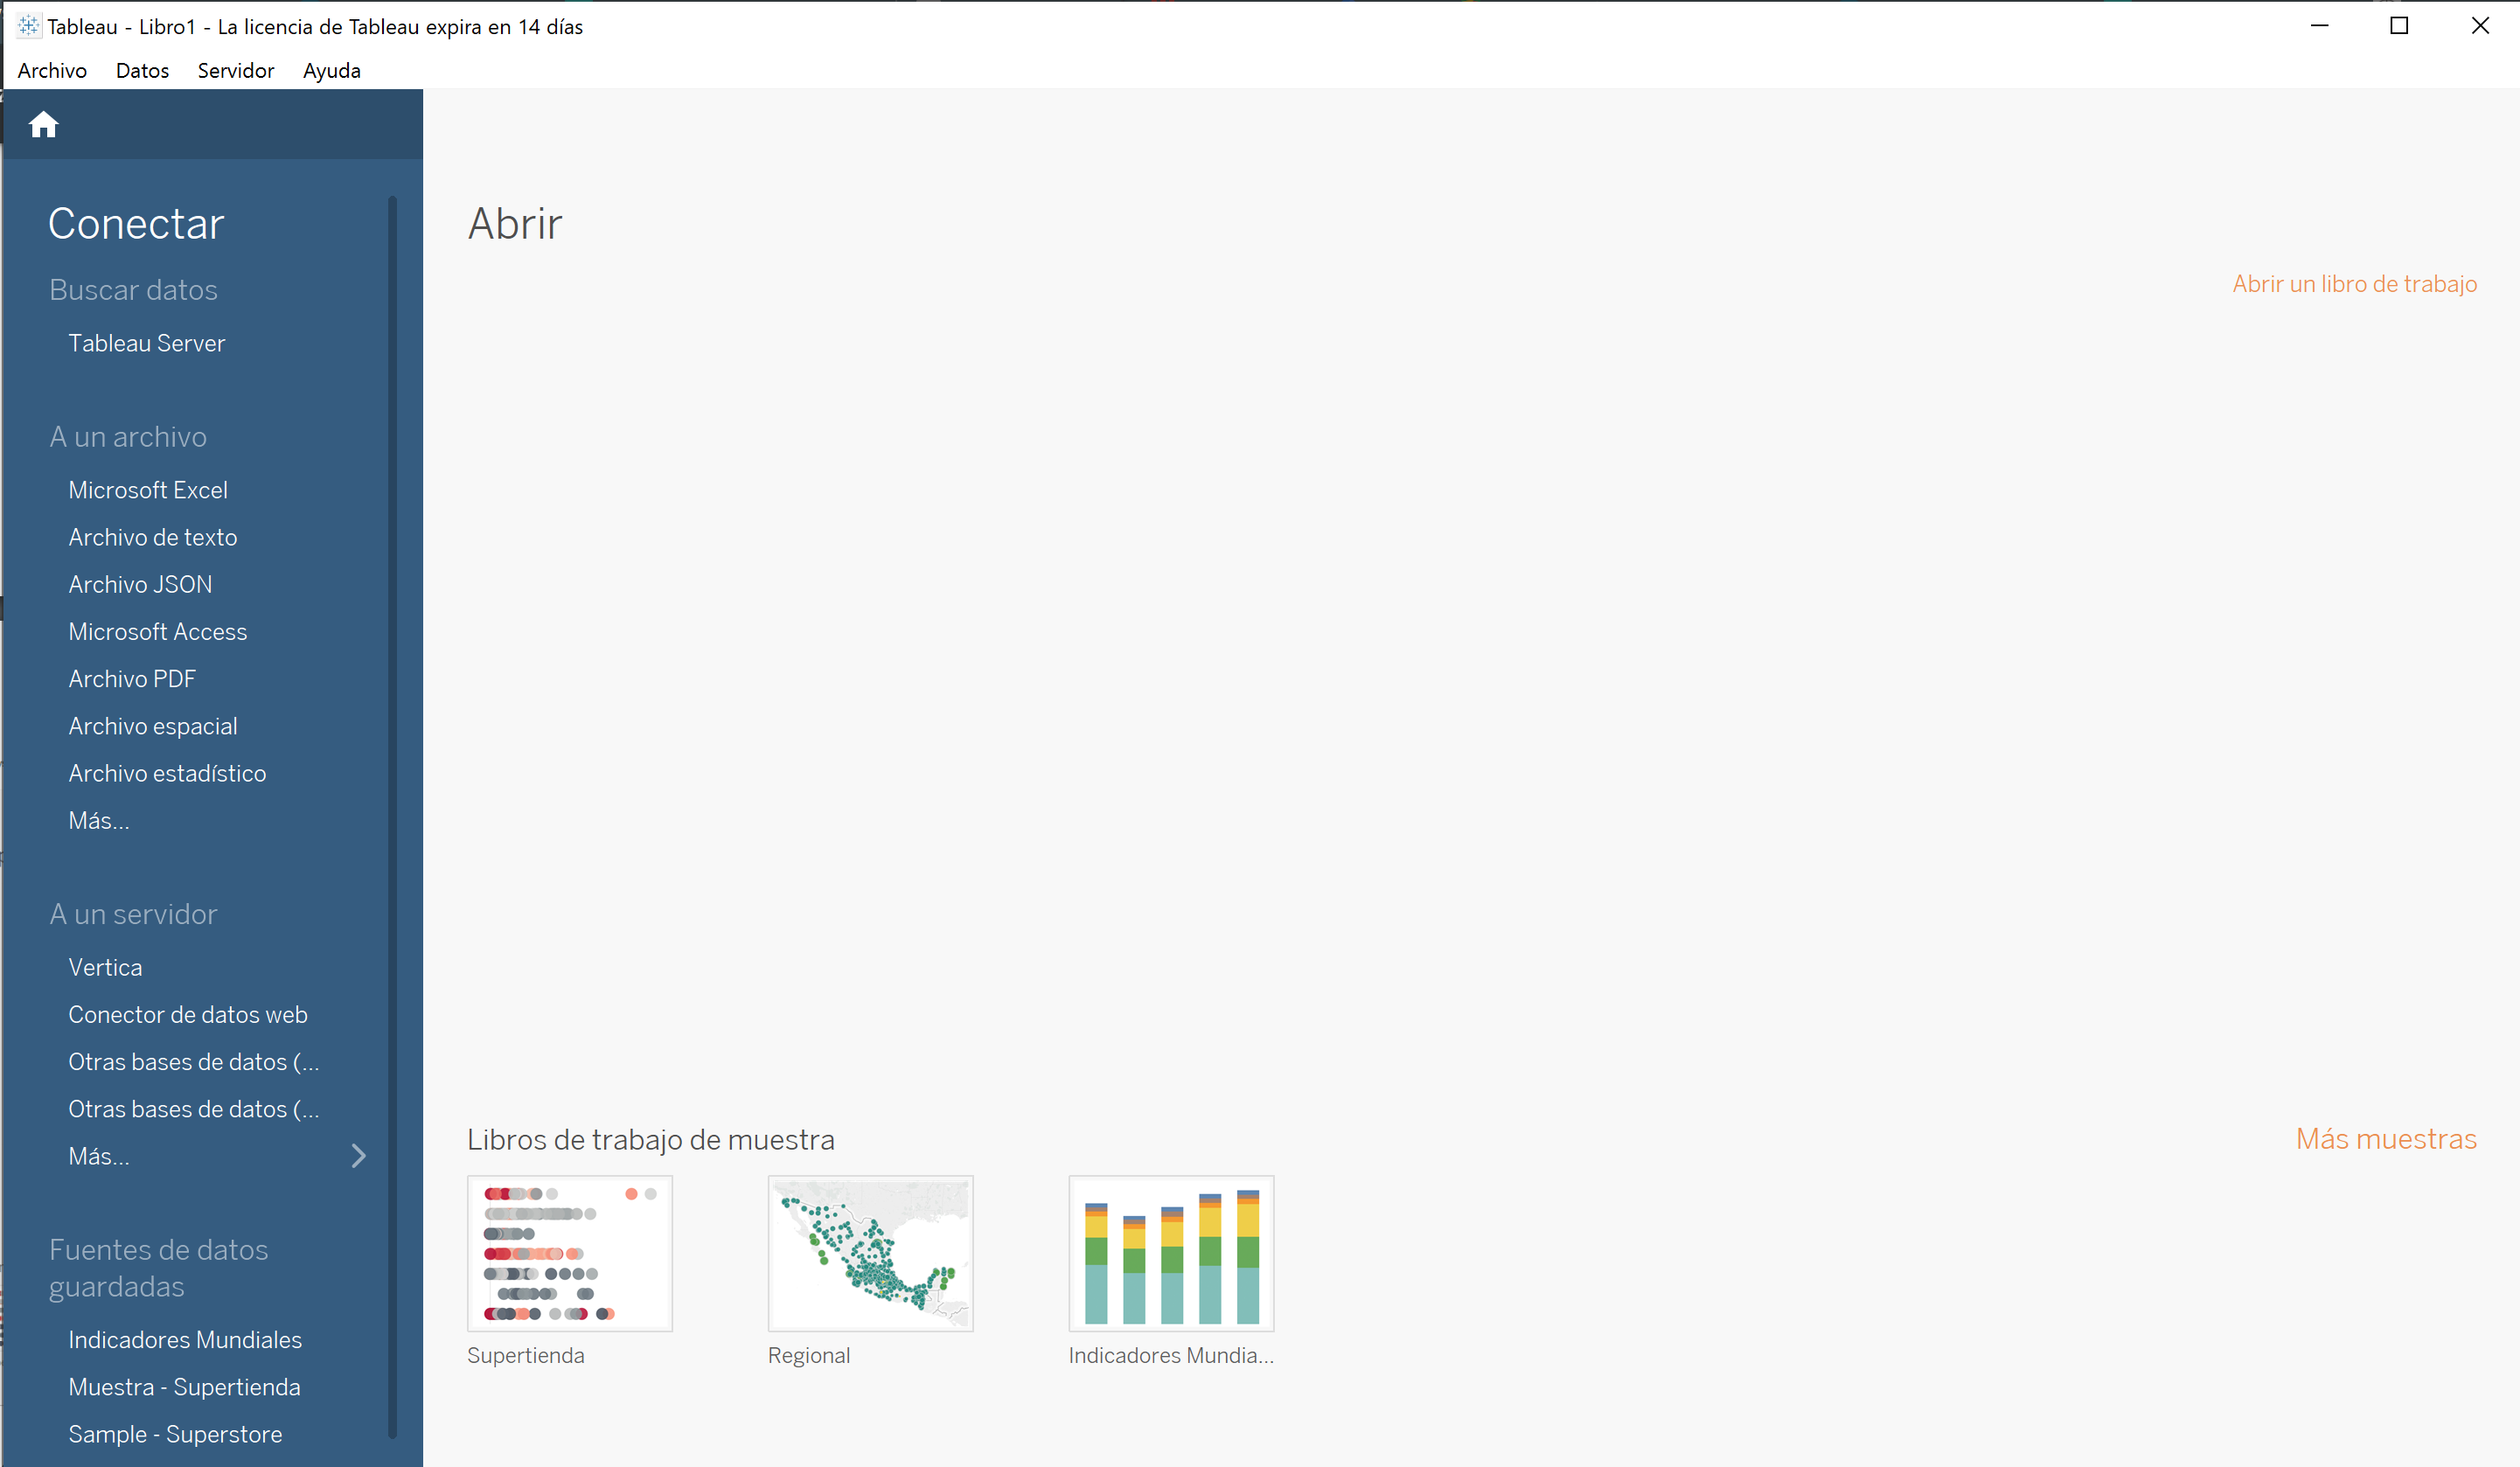
\includegraphics[width=16cm]{img/1.png}  
\end{center}

\section{Comenzar}
En esta sección, aprenderemos algunas operaciones básicas en Tableau para acostumbrarnos a su
interfaz. 
\subsection{Espacio de trabajo de Tableau}
El espacio de trabajo de Tableau es una colección de hojas de trabajo, barra de menú, barra de
herramientas, tarjeta de marcas, estantes y muchos otros elementos sobre los que aprenderemos en las
próximas secciones. Las hojas pueden ser hojas de trabajo, paneles o historias. La siguiente imagen
destaca los componentes principales del espacio de trabajo. Sin embargo, se logrará una mayor
familiaridad una vez que trabajemos con datos reales.
\begin{center}
    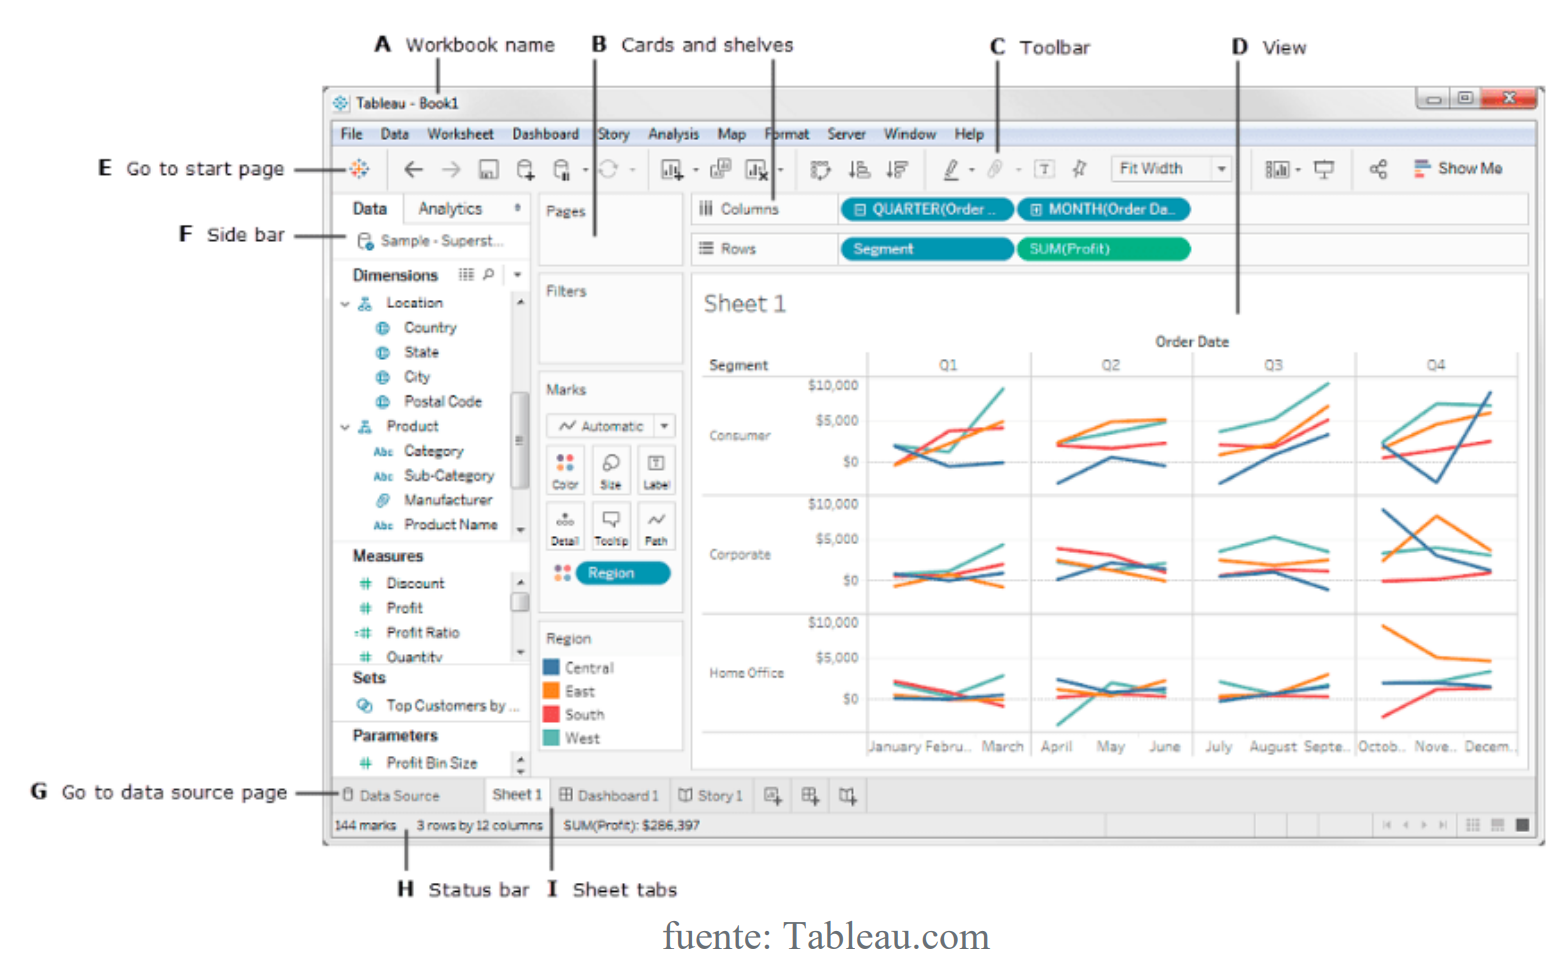
\includegraphics[width=16cm]{img/2.png}  
\end{center}

\subsection{Conexión a una fuente de datos}
Para comenzar a trabajar con Tableau, debemos conectar Tableau a la fuente de datos. Tableau es
compatible con muchas fuentes de datos. Las fuentes de datos compatibles con Tableau aparecen en el
lado izquierdo de la pantalla inicial. Algunas fuentes de datos de uso común son Excel, archivos de
texto, bases de datos relacionales o incluso en un servidor. También se puede conectar a una fuente de
base de datos en la nube como Google Analytics, Amazon Redshift, etc.
\\\\La pantalla de inicio de Tableau Desktop muestra las fuentes de datos disponibles que también se
pueden conectar. También depende de la versión de Tableau, ya que la versión de pago ofrece más
posibilidades. En el lado izquierdo de la pantalla, hay un Connectpanel que resalta las fuentes
disponibles. Los tipos de archivo se enumeran primero, seguidos de los tipos de servidor comunes o los
servidores que se han conectado recientemente. Puede abrir libros de trabajo creados previamente en
la Openpestaña Bajo . Tableau Desktop también proporciona algunos libros de trabajo de muestra a
continuación Sample Workbooks.
\begin{center}
    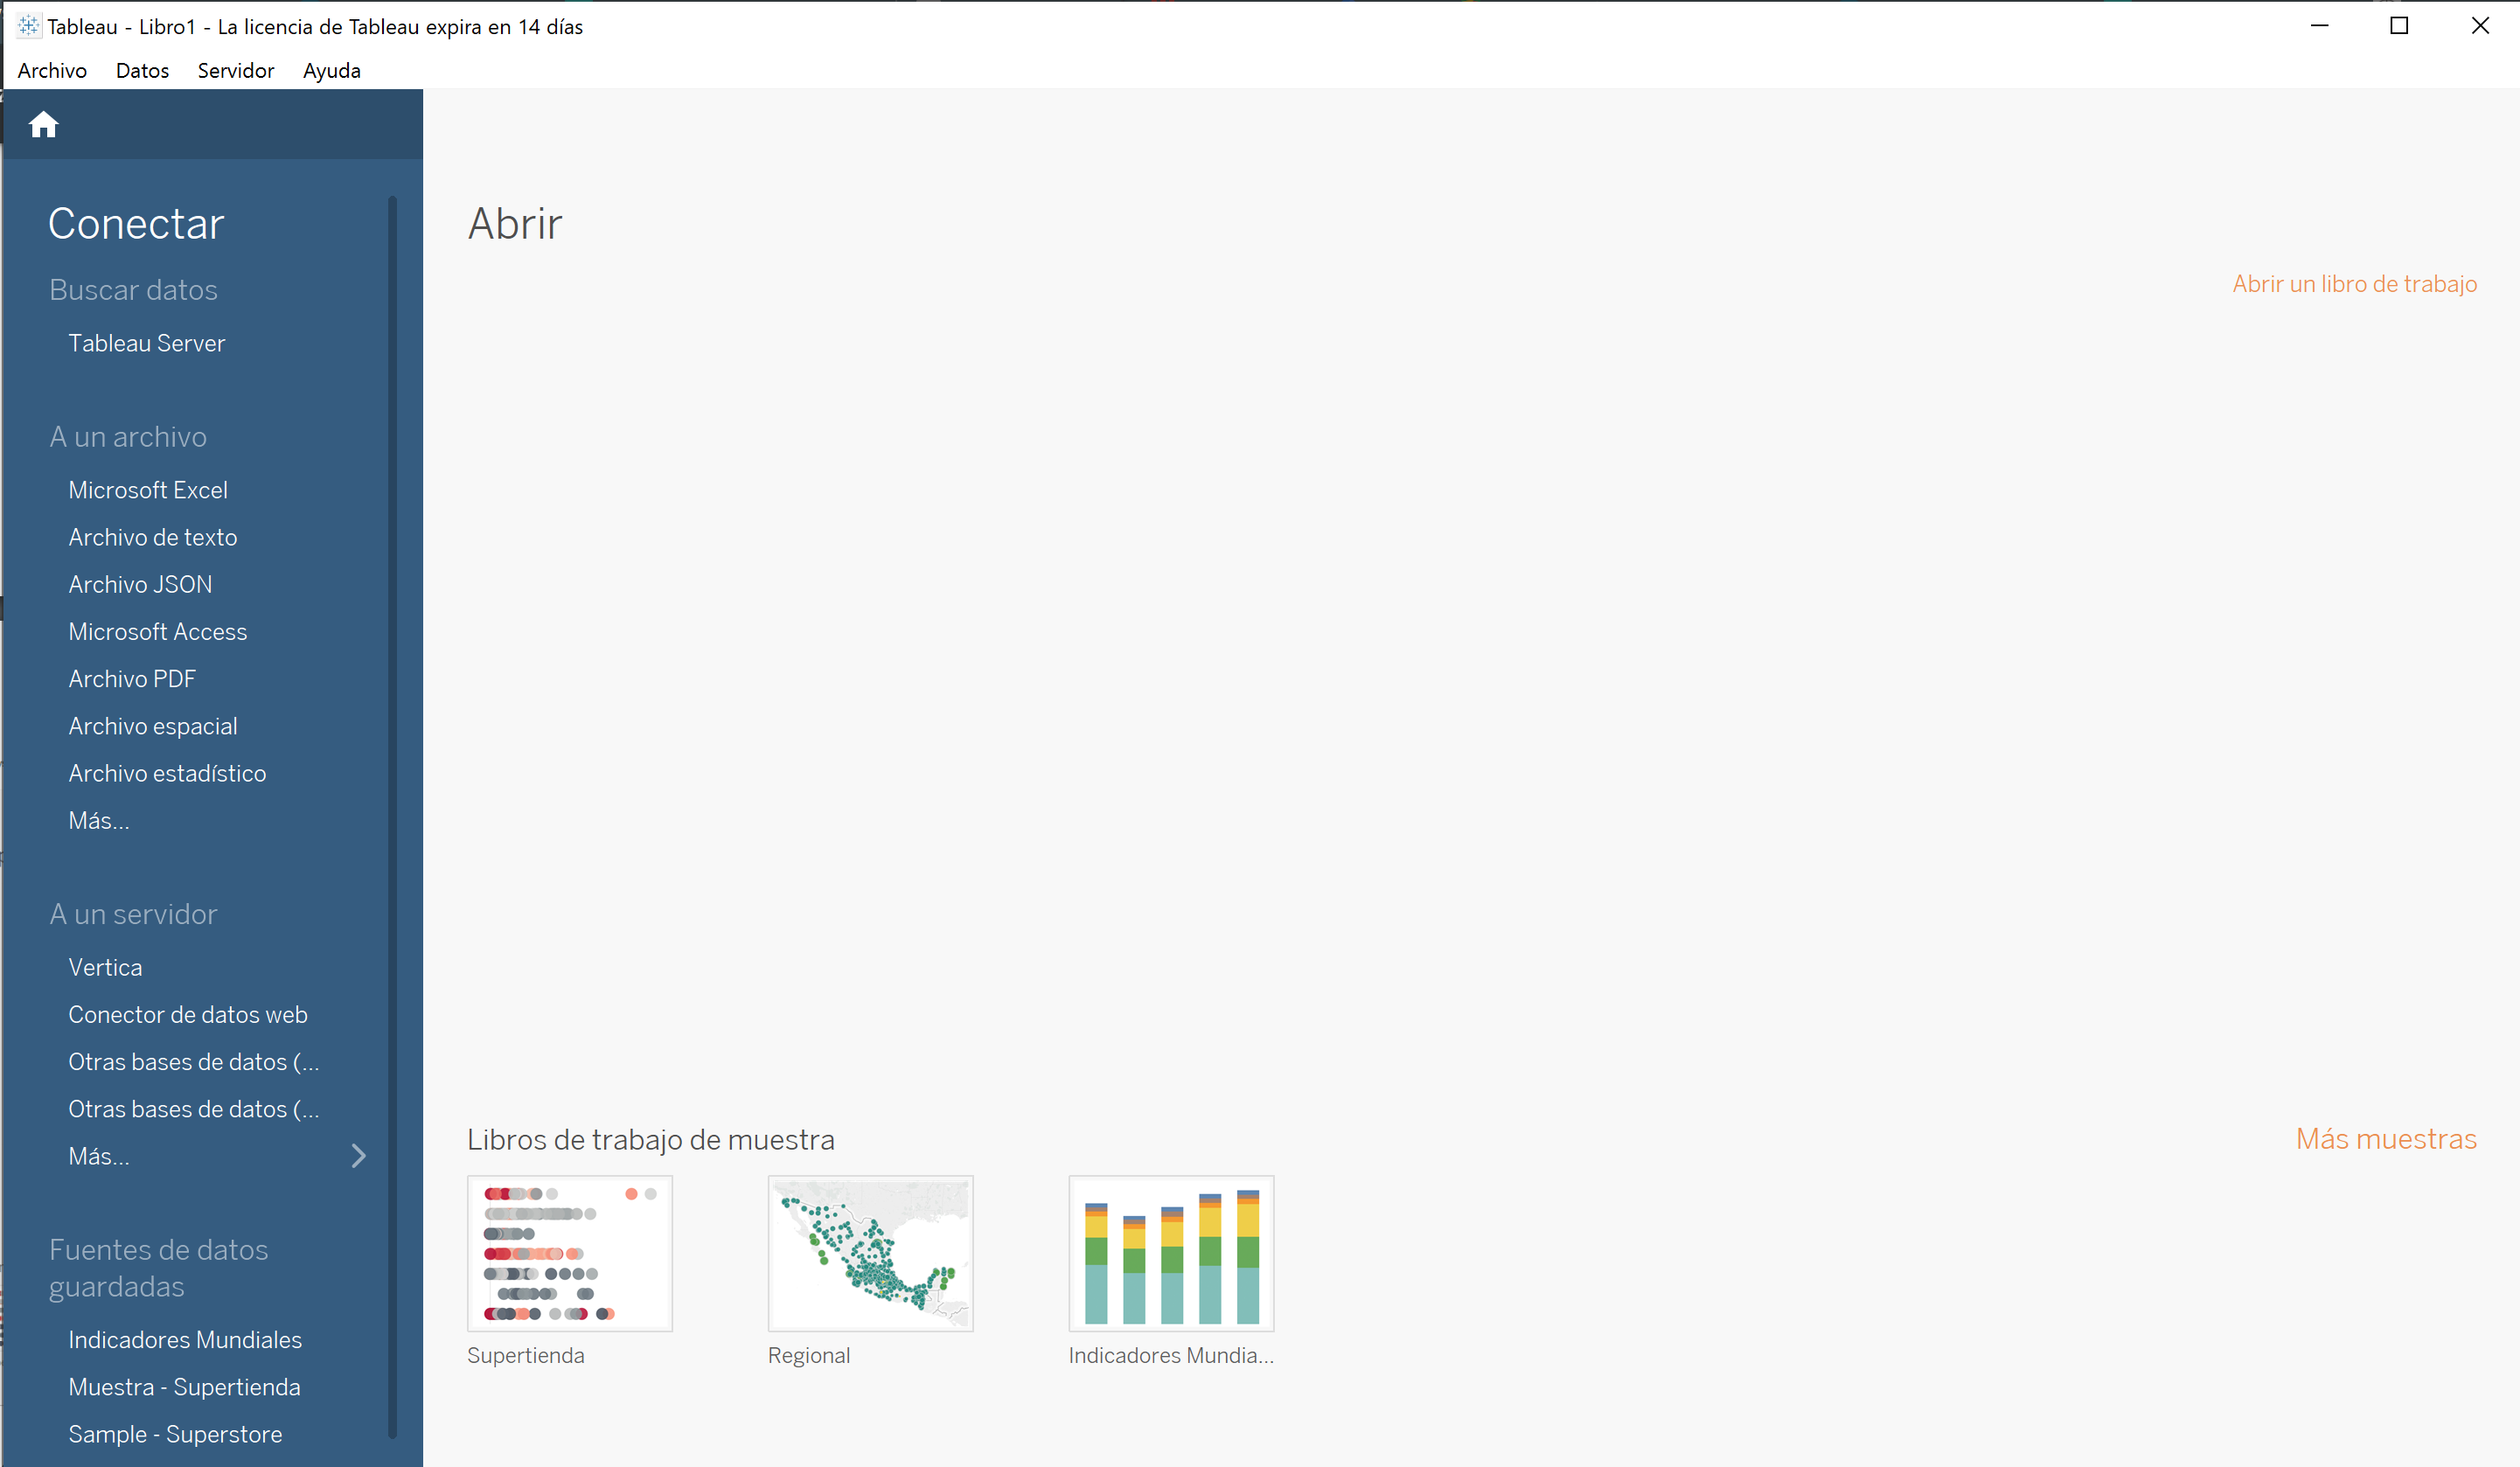
\includegraphics[width=16cm]{img/1.png}  
\end{center}
Conexión al conjunto de datos Sample-Superstore
\\\\Trabajaremos con un conjunto de datos de muestra con nombres Superstore dataset , que viene
precargado con Tableau. Sin embargo, descargaremos el archivo desde aquí para que podamos tener
una idea de cómo conectarnos a una fuente de datos de Excel. Los datos son los de un
hipermercado. Contiene información sobre productos, ventas, beneficios, etc. Nuestro objetivo como
analistas de datos es analizar los datos y encontrar áreas críticas de mejora dentro de esta empresa
ficticia.
\\\\STEPS:
\\\\1. Importe los datos al espacio de trabajo de Tableau desde la computadora.
\\\\2. En la pestaña Hojas, se verán tres hojas: Pedidos, Personas y Devoluciones. Sin embargo, nos
centraremos solo en los datos de los pedidos. Haga doble clic en Hoja de pedidos y se abrirá
como una hoja de cálculo.
\begin{center}
    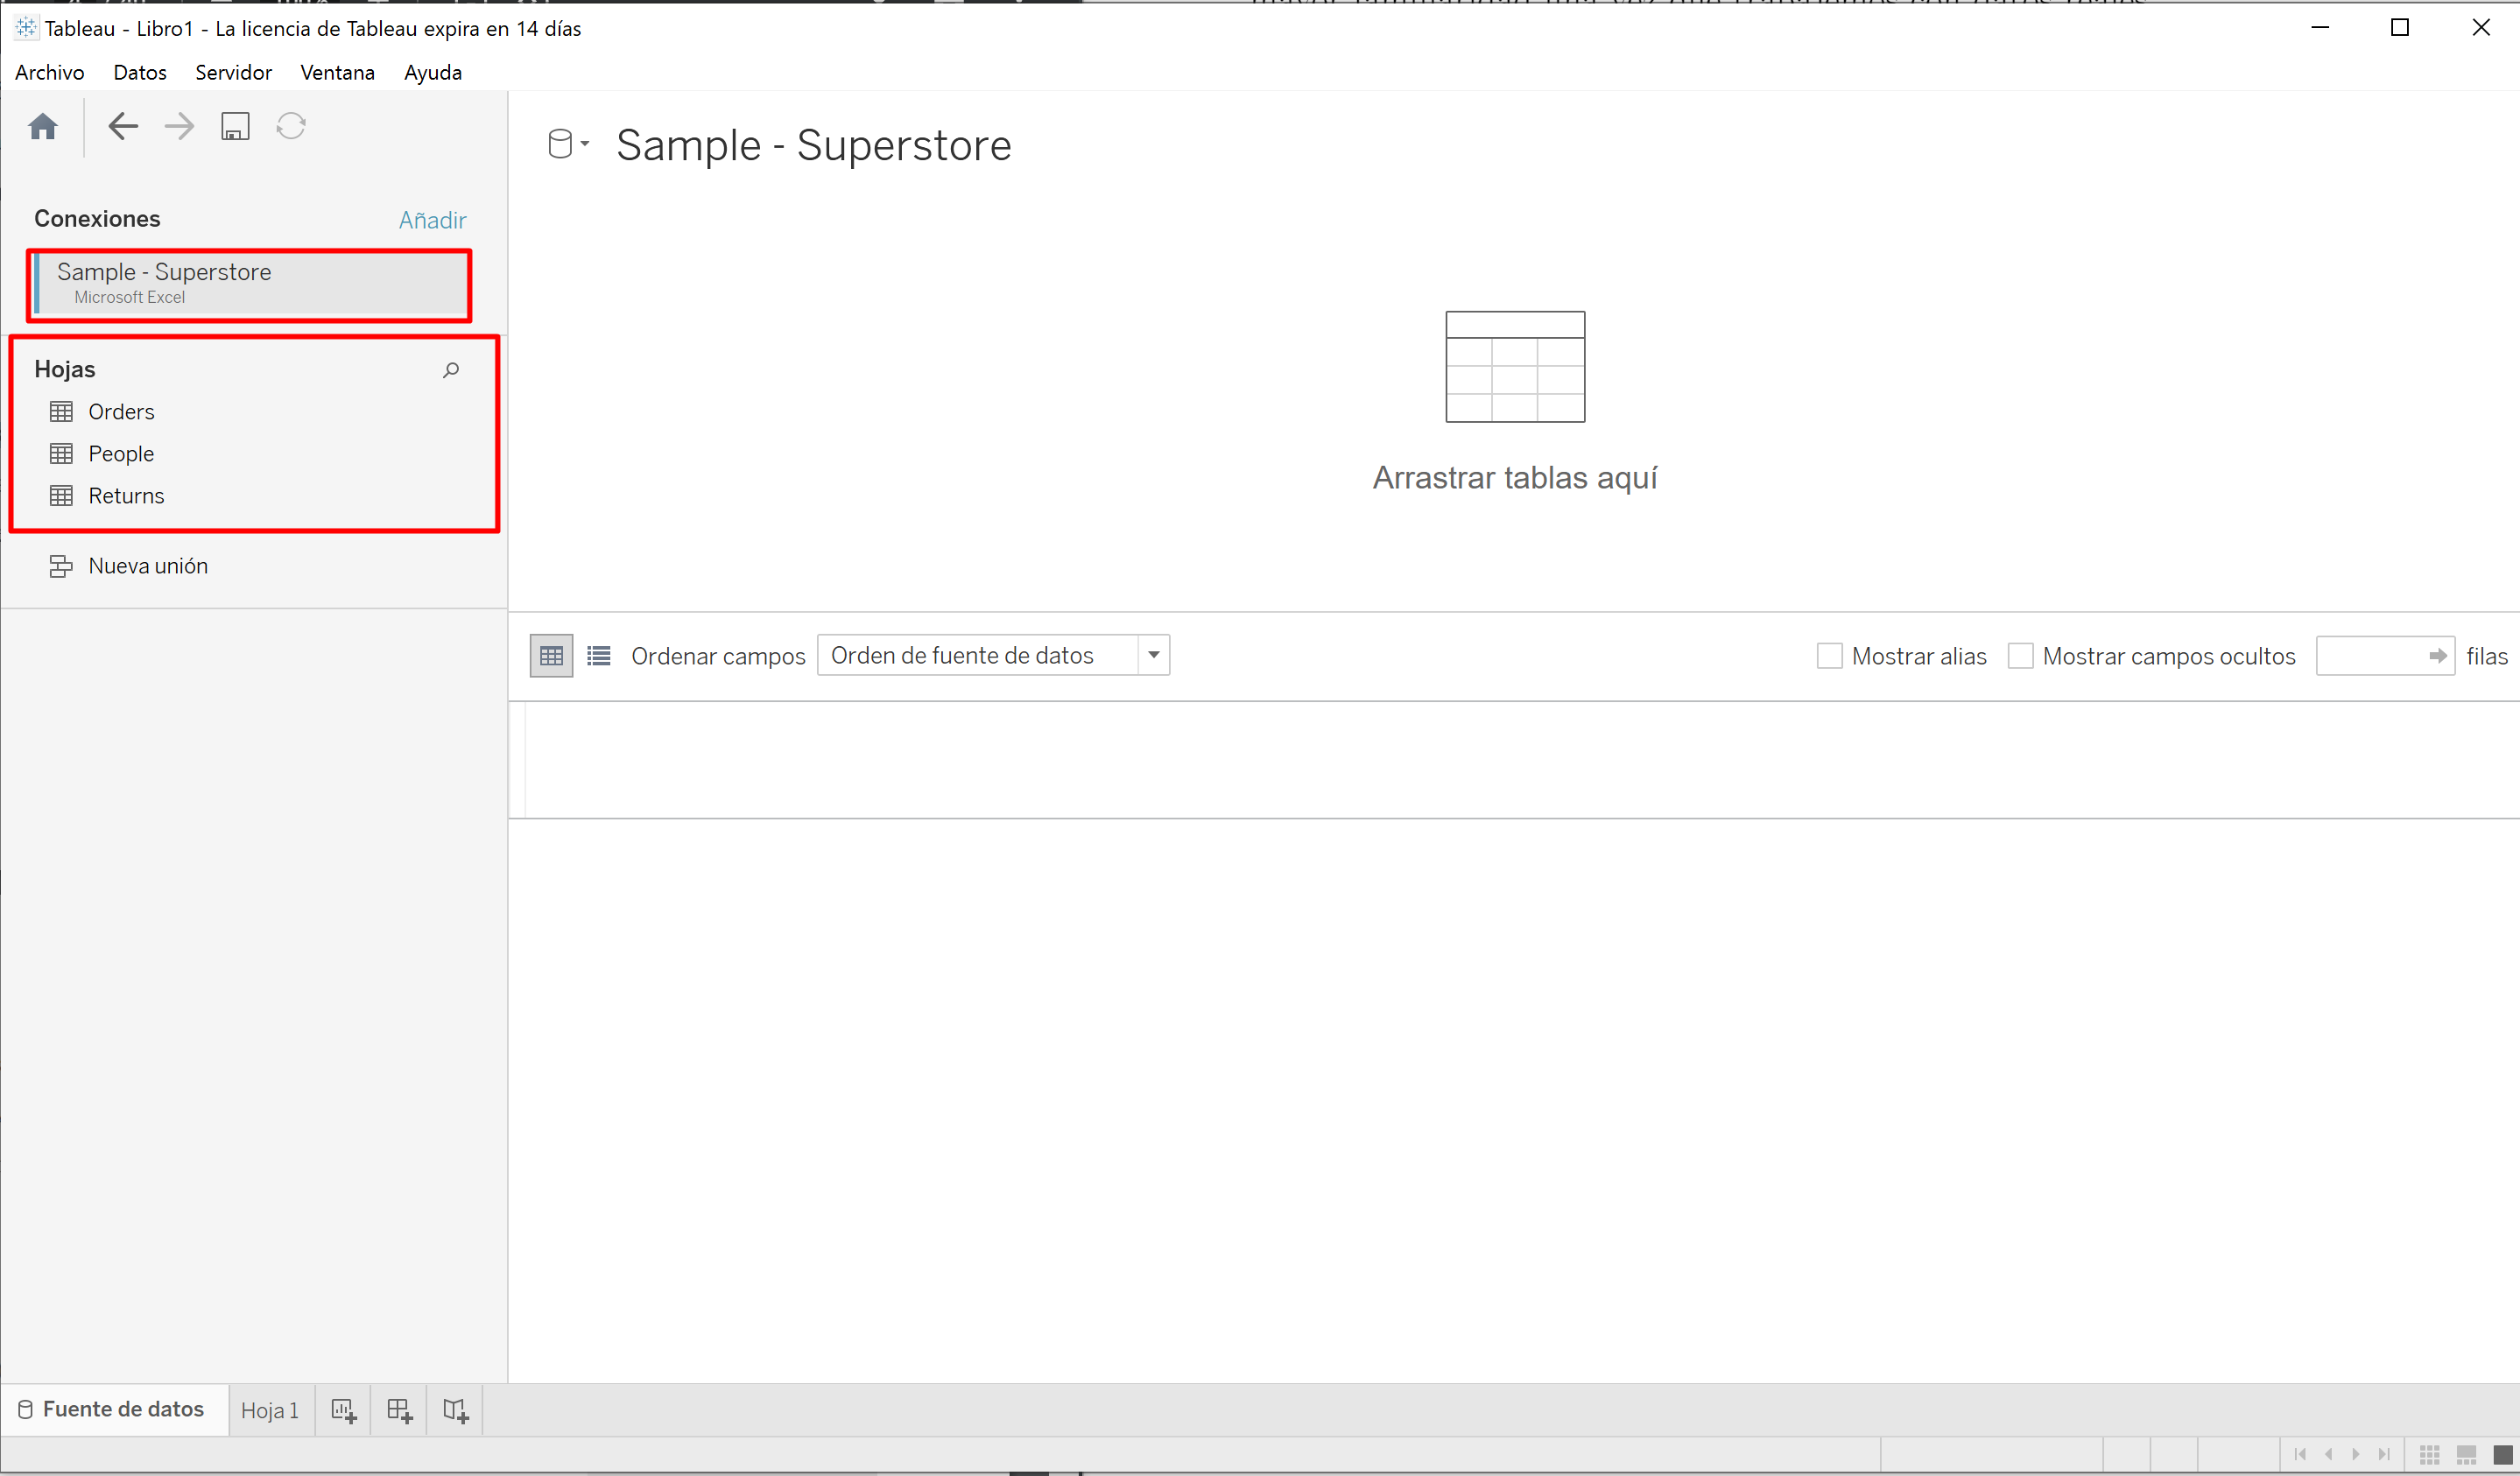
\includegraphics[width=16cm]{img/3.png}  
\end{center}
\begin{center}
    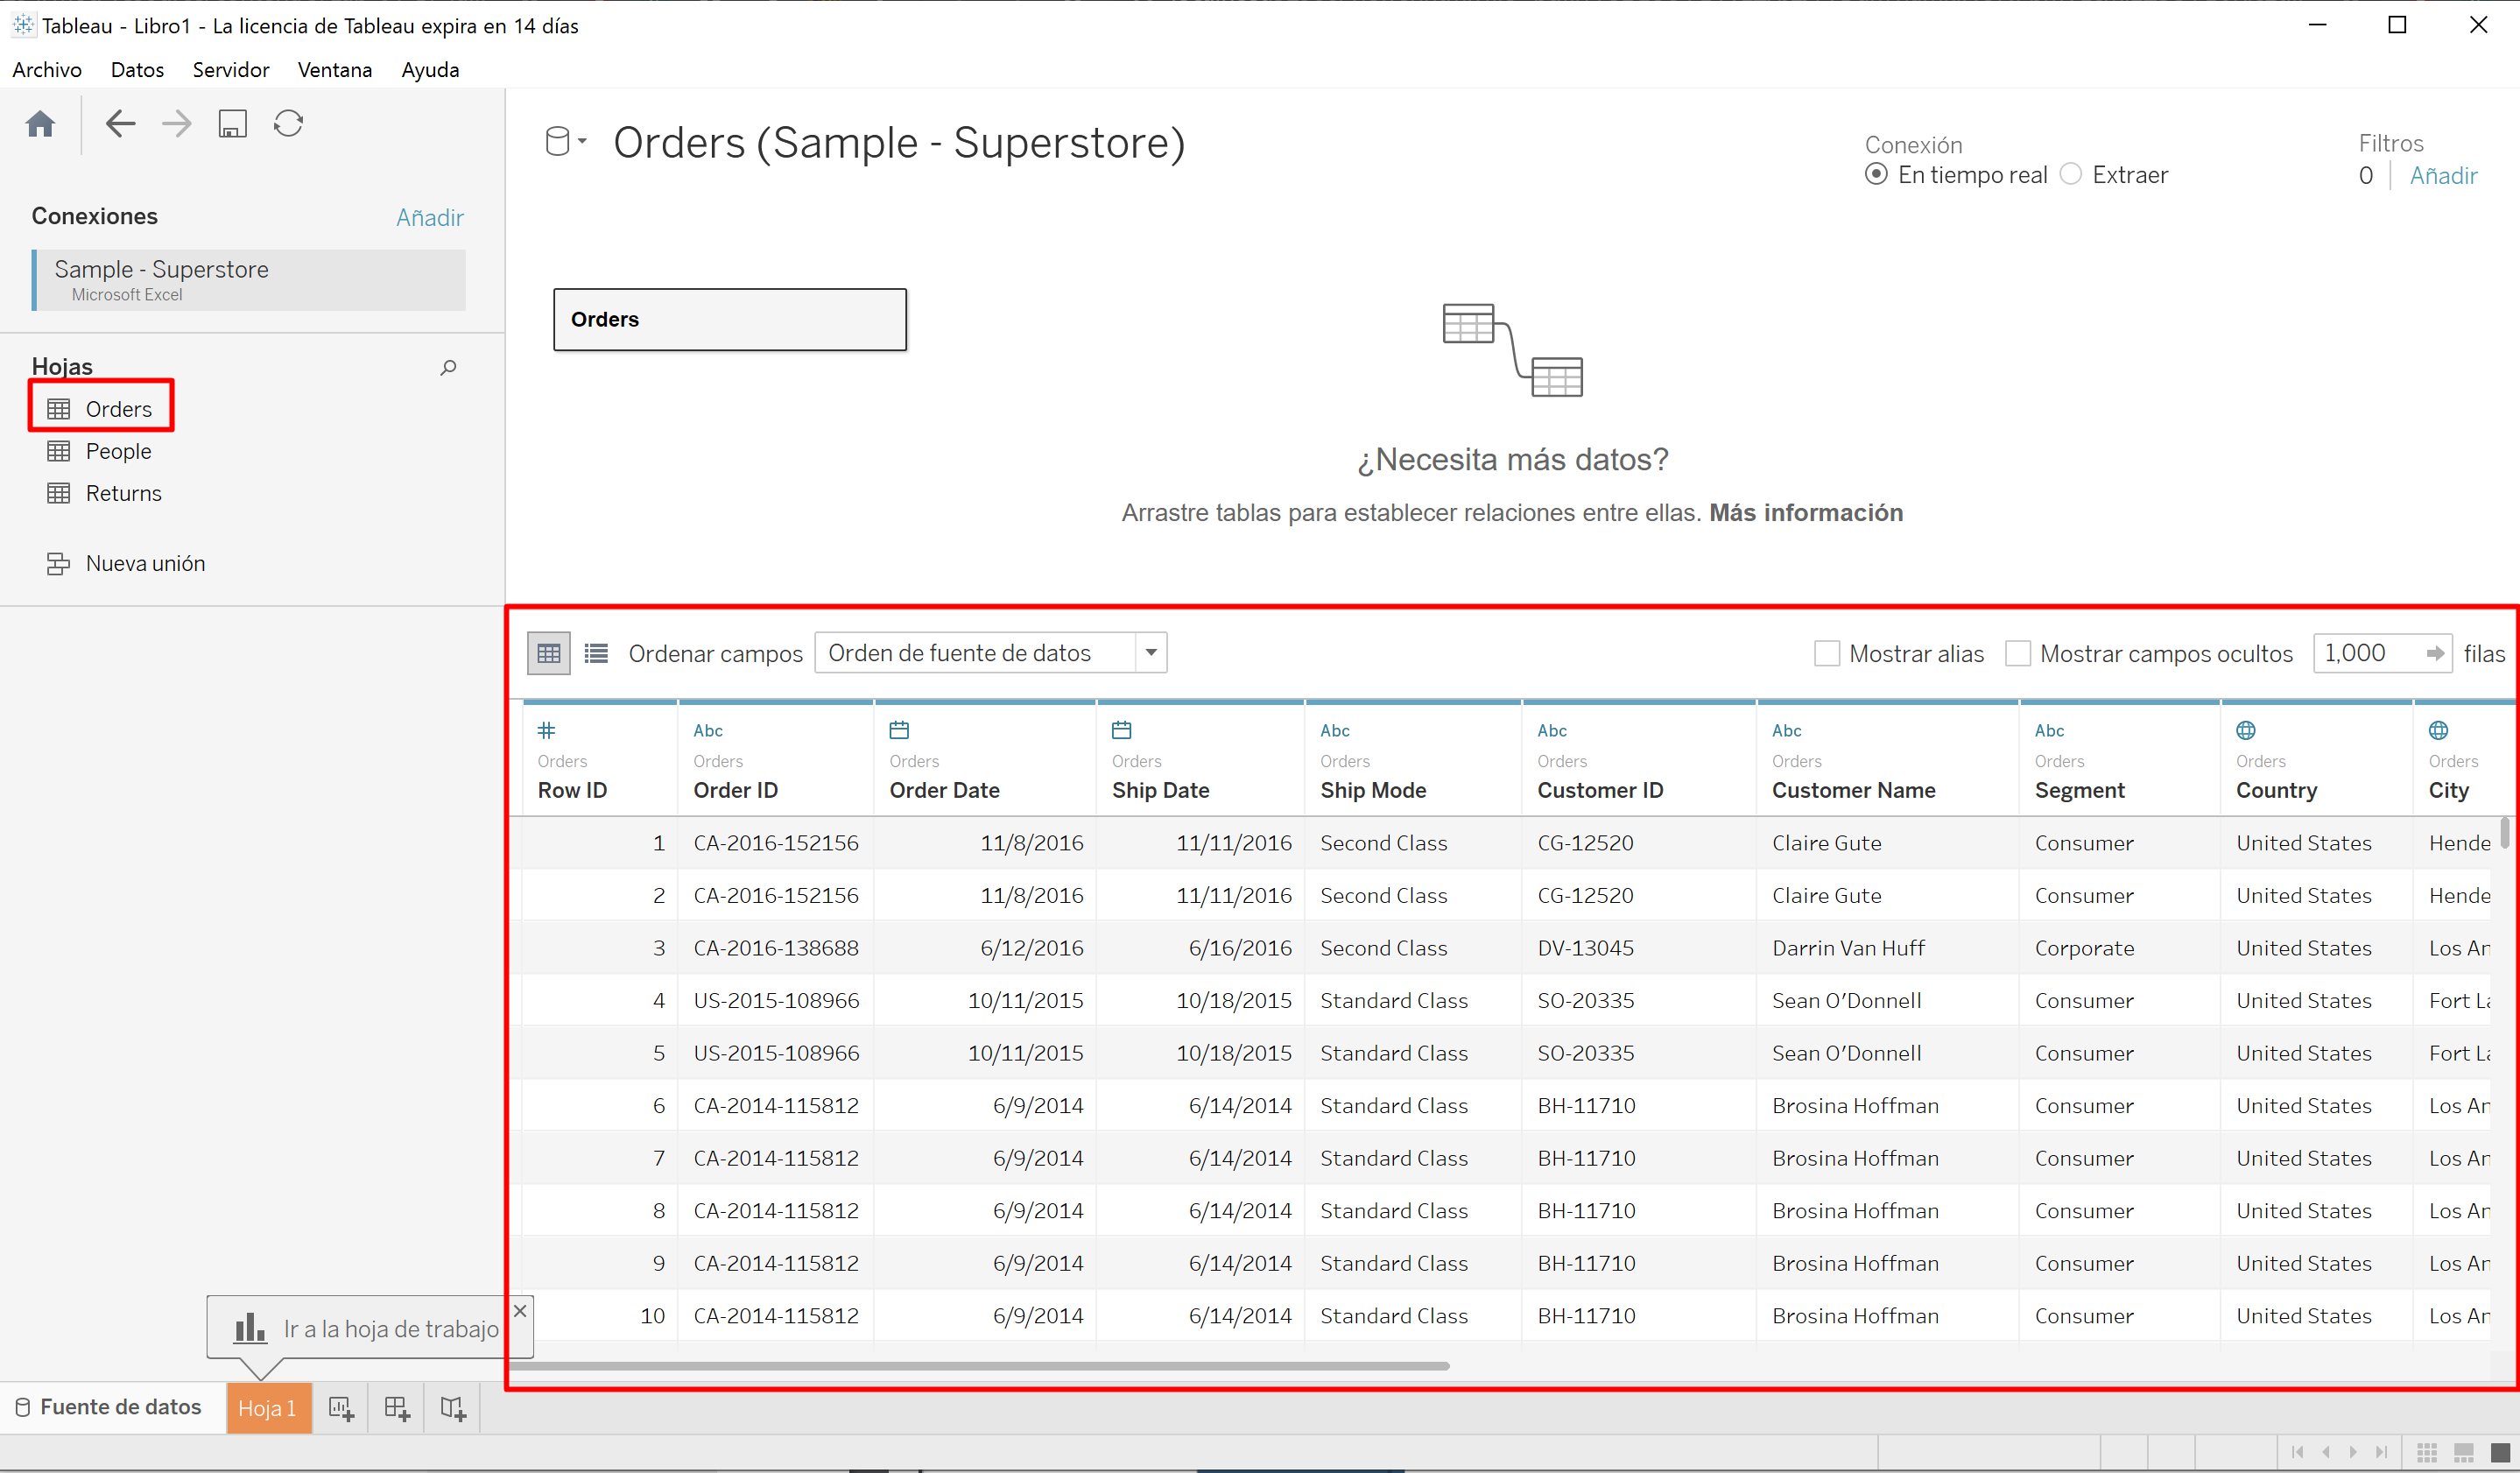
\includegraphics[width=16cm]{img/4.png}  
\end{center}
3. Observamos que las primeras tres filas de datos se ven un poco diferentes y no están en el
formato deseado. Aquí utilizamos el intérprete de datos , también presente en la pestaña
Hojas. Al hacer clic en él, obtenemos una hoja con un formato agradable.
\begin{center}
    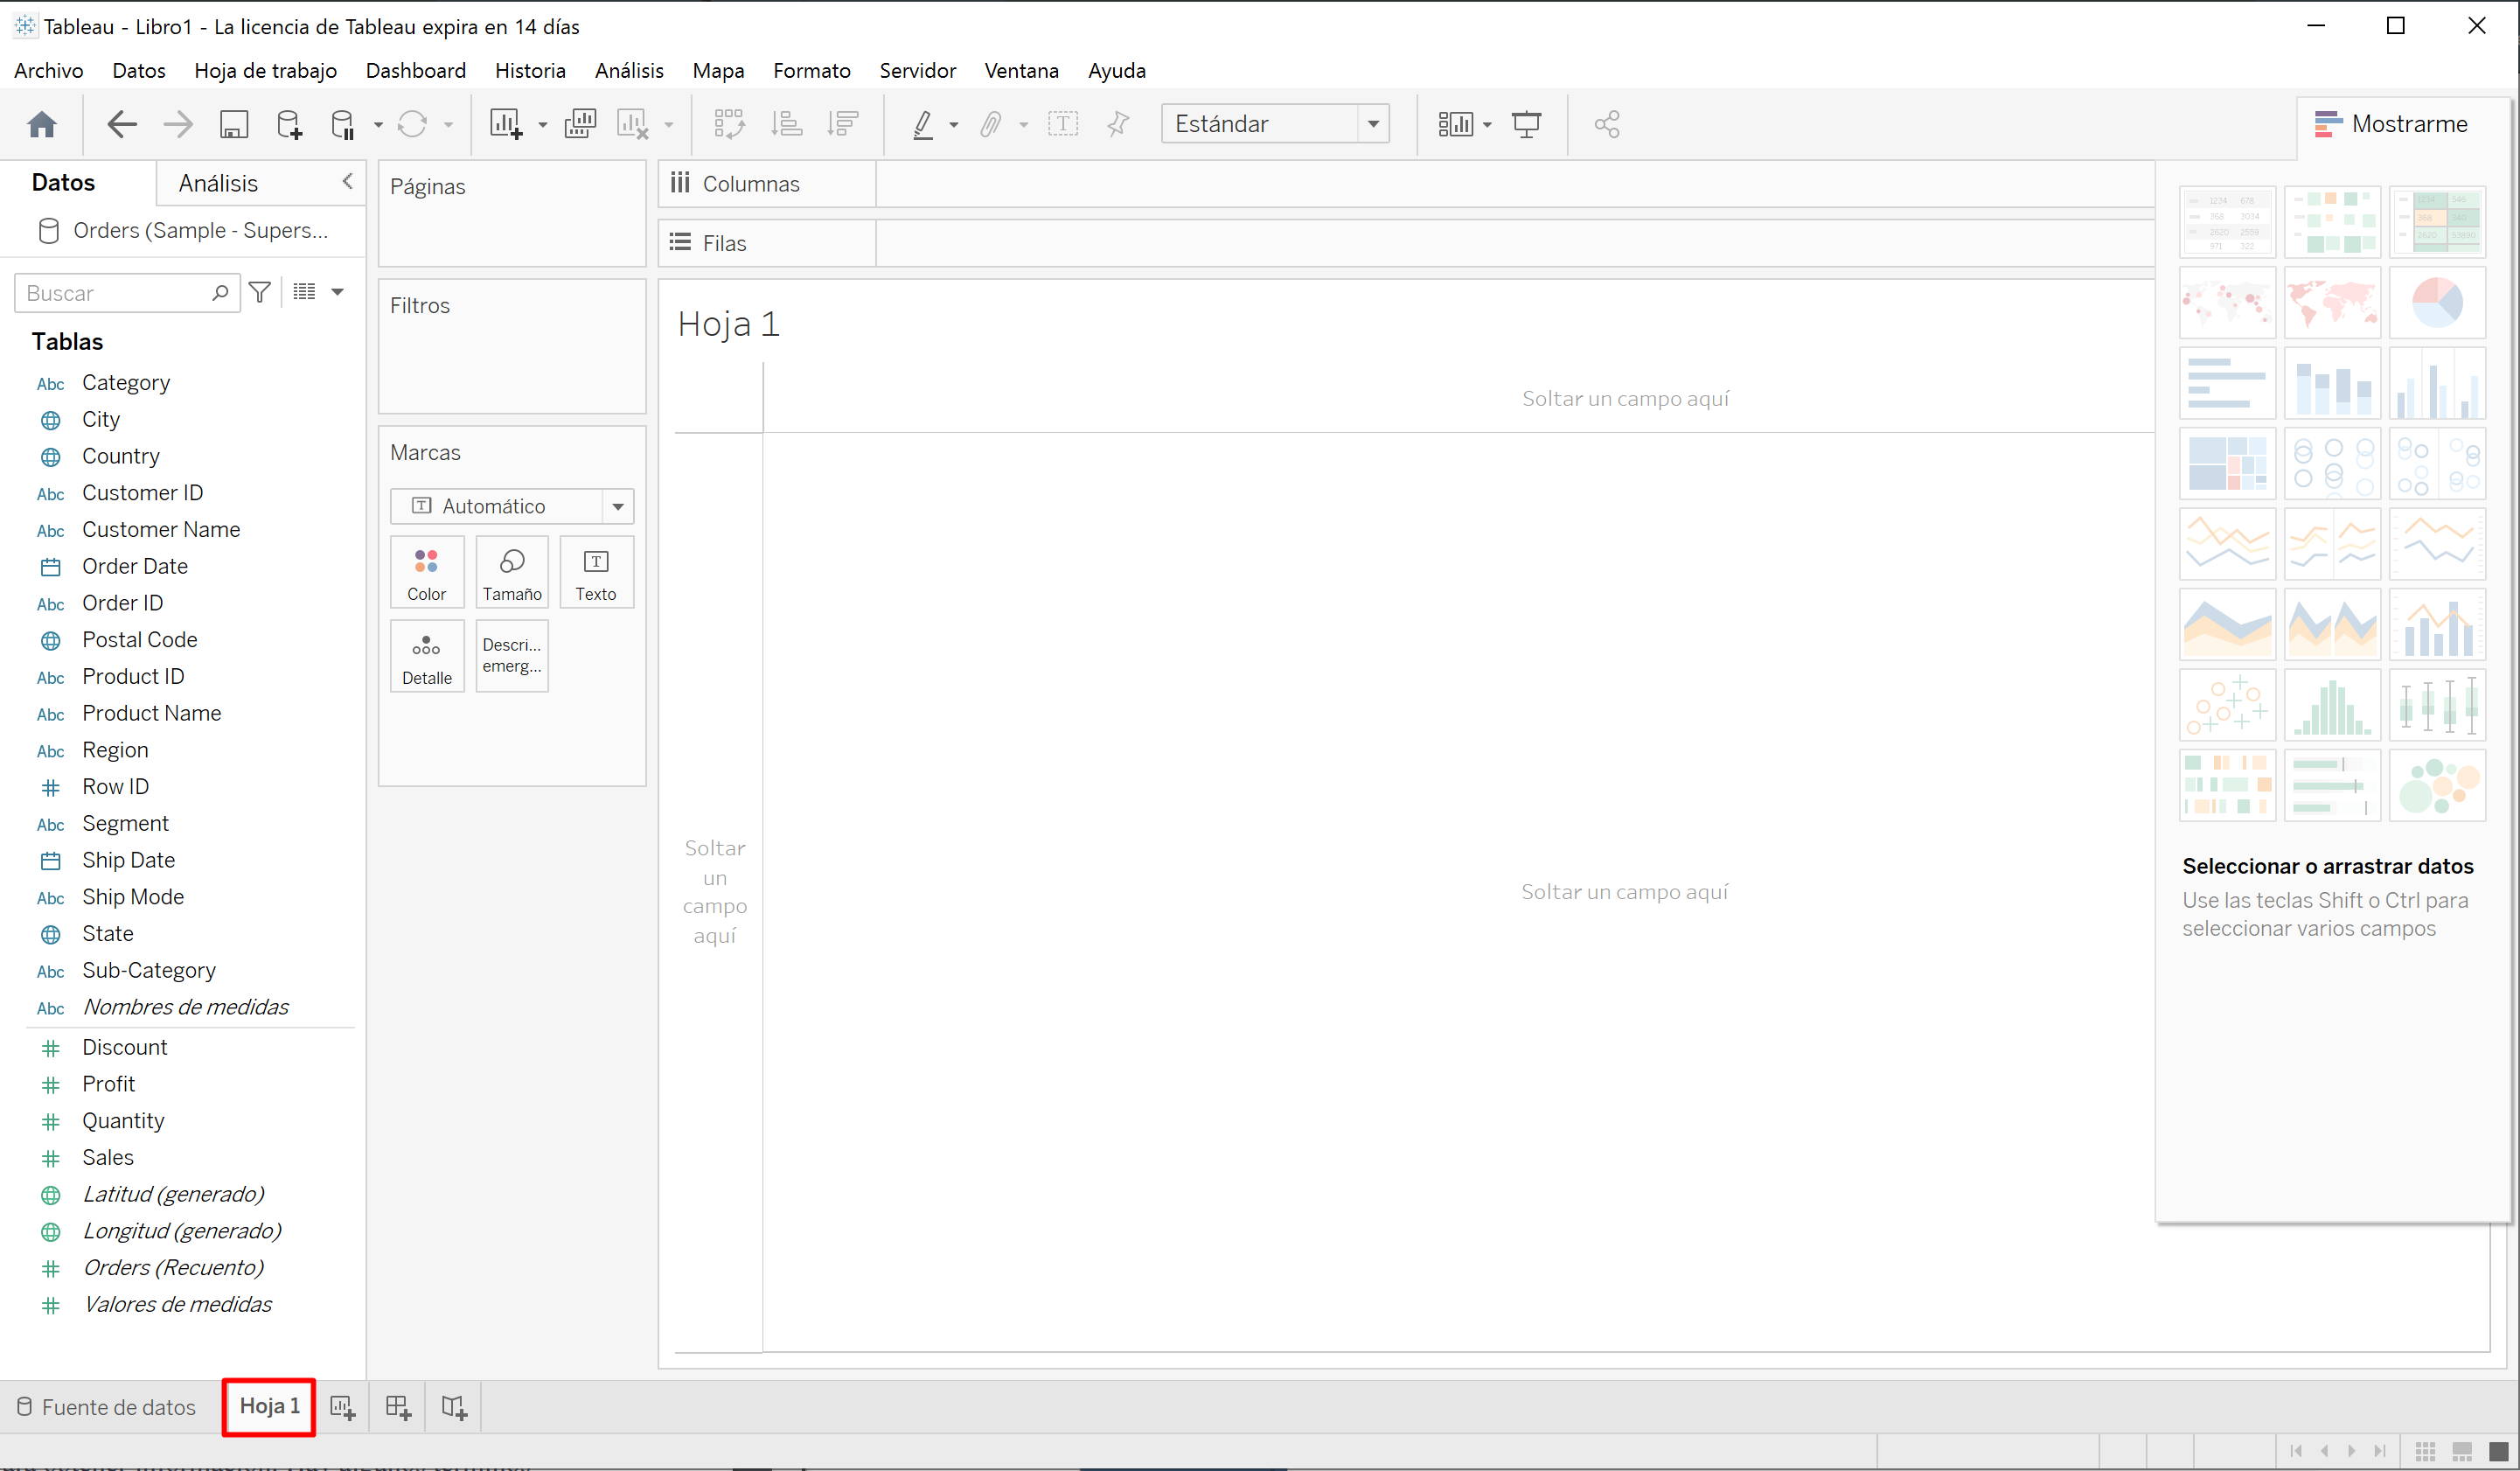
\includegraphics[width=16cm]{img/5.png}
    \vspace{1cm}  
\end{center}

\subsection{Crear una vista}
Comenzaremos generando un gráfico simple. En esta sección, conoceremos nuestros datos y
comenzaremos a hacer preguntas sobre los datos para obtener información. Hay algunos términos
importantes que encontraremos en esta sección.
\\\\Dimension
\\\\Measures
\\\\Aggregation
\\\\Las dimensiones: son datos cualitativos, como un nombre o una fecha. De forma predeterminada,
Tableau clasifica automáticamente los datos que contienen información cualitativa o categórica como
una dimensión, por ejemplo, cualquier campo con texto o valores de fecha. Estos campos generalmente
aparecen como encabezados de columna para filas de datos, como Nombre del cliente o Fecha del
pedido, y también definen el nivel de granularidad que se muestra en la vista.
\\\\Las medidas: son datos numéricos cuantitativos. De forma predeterminada, Tableau trata cualquier
campo que contenga este tipo de datos como una medida, por ejemplo, transacciones de ventas o
ganancias. Los datos que se clasifican como una medida se pueden agregar en función de una
dimensión determinada, por ejemplo, las ventas totales (medida) por región (dimensión).
\\\\La agregación: son los datos a nivel de fila acumulados en una categoría superior, como la suma de las
ventas o el beneficio total.
\\\\Tableau ordena automáticamente los campos en Medidas y Dimensiones. Sin embargo, para cualquier
anomalía, también se puede cambiar manualmente.
\\\\STEPS:
\\\\1. Vaya a la hoja de trabajo. Haga clic en la pestaña Sheet 1 en la parte inferior izquierda del
espacio de trabajo del cuadro.
\\\\2. Una vez que esté en la hoja de trabajo, desde Dimensionsdebajo del panel Datos,
arrastre Order Dateal estante Columna.
\begin{center}
    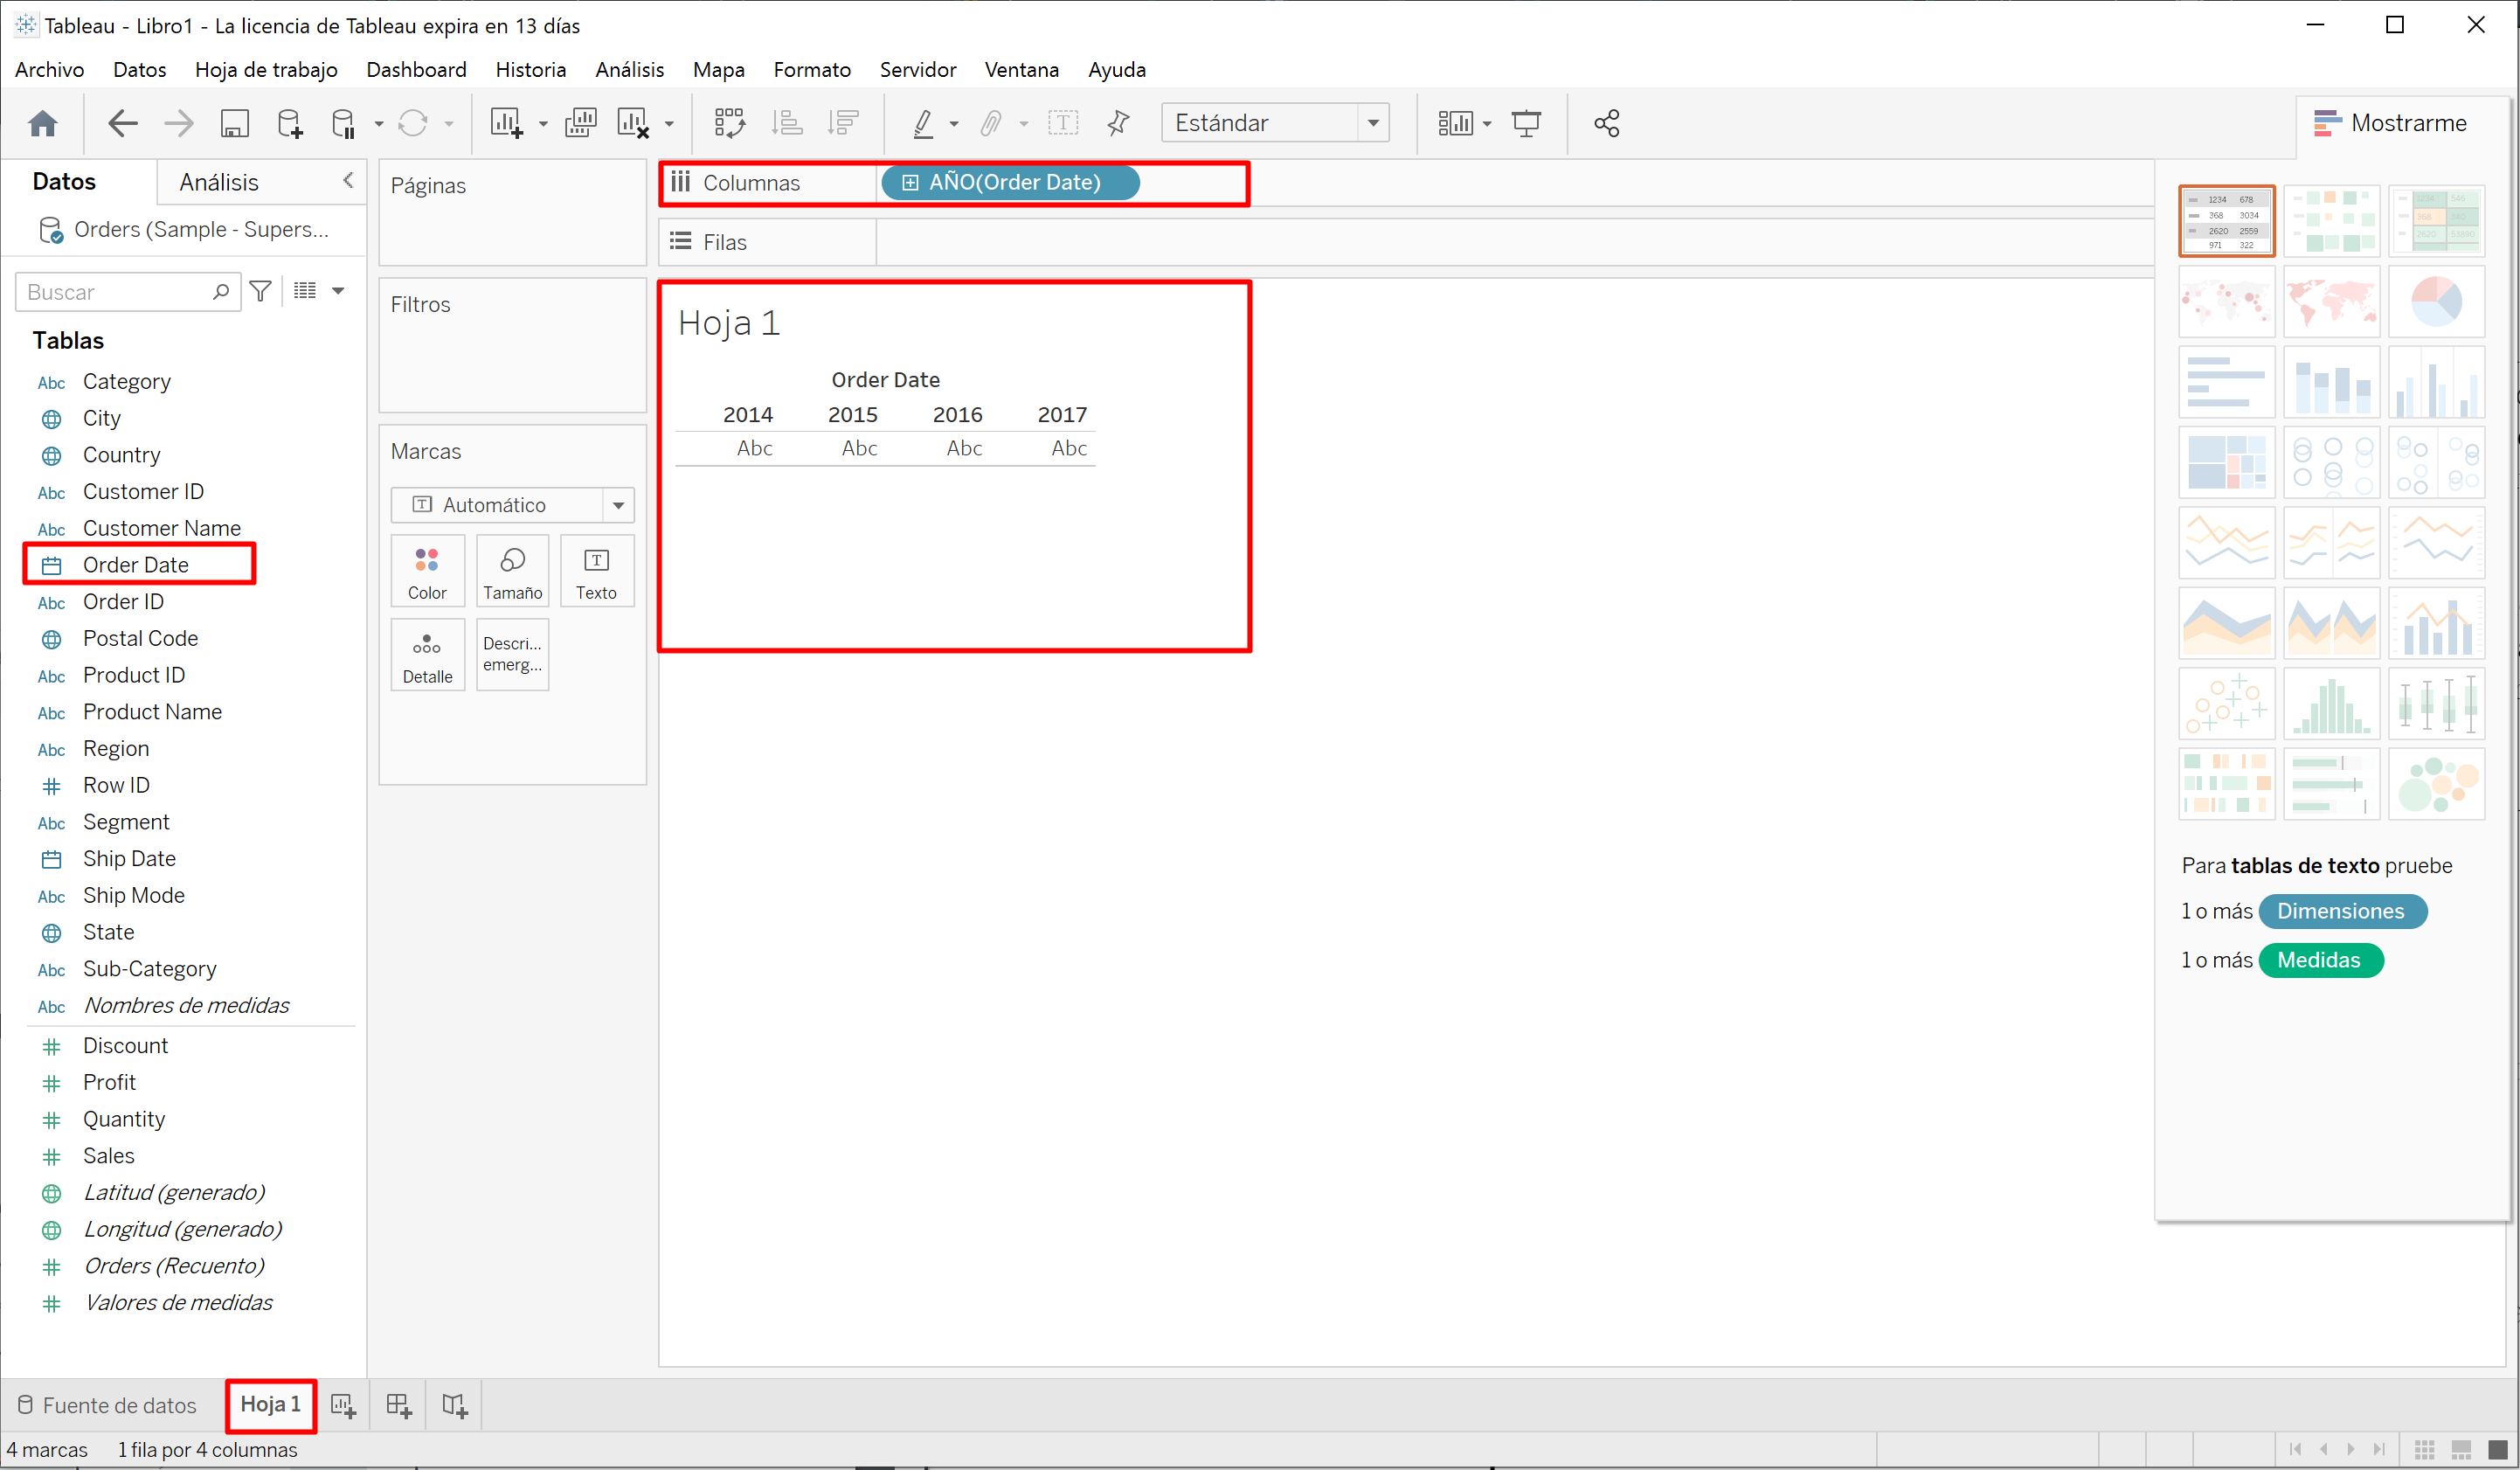
\includegraphics[width=16cm]{img/6.png}  
\end{center}
Al arrastrar el Order Date al estante de columnas, se crea una columna para cada año de
pedidos en el conjunto de datos. Un indicador 'Abc' está visible debajo de cada columna, lo que
implica que se pueden arrastrar aquí texto o datos numéricos o de texto. Por otro lado, si
tiramos de Salesaquí, se crearía una tabla de referencias cruzadas que mostraría las ventas
totales de cada año.
\\\\3. Del mismo modo, desde la Measurespestaña, arrastre el Salescampo al estante Filas.
\begin{center}
    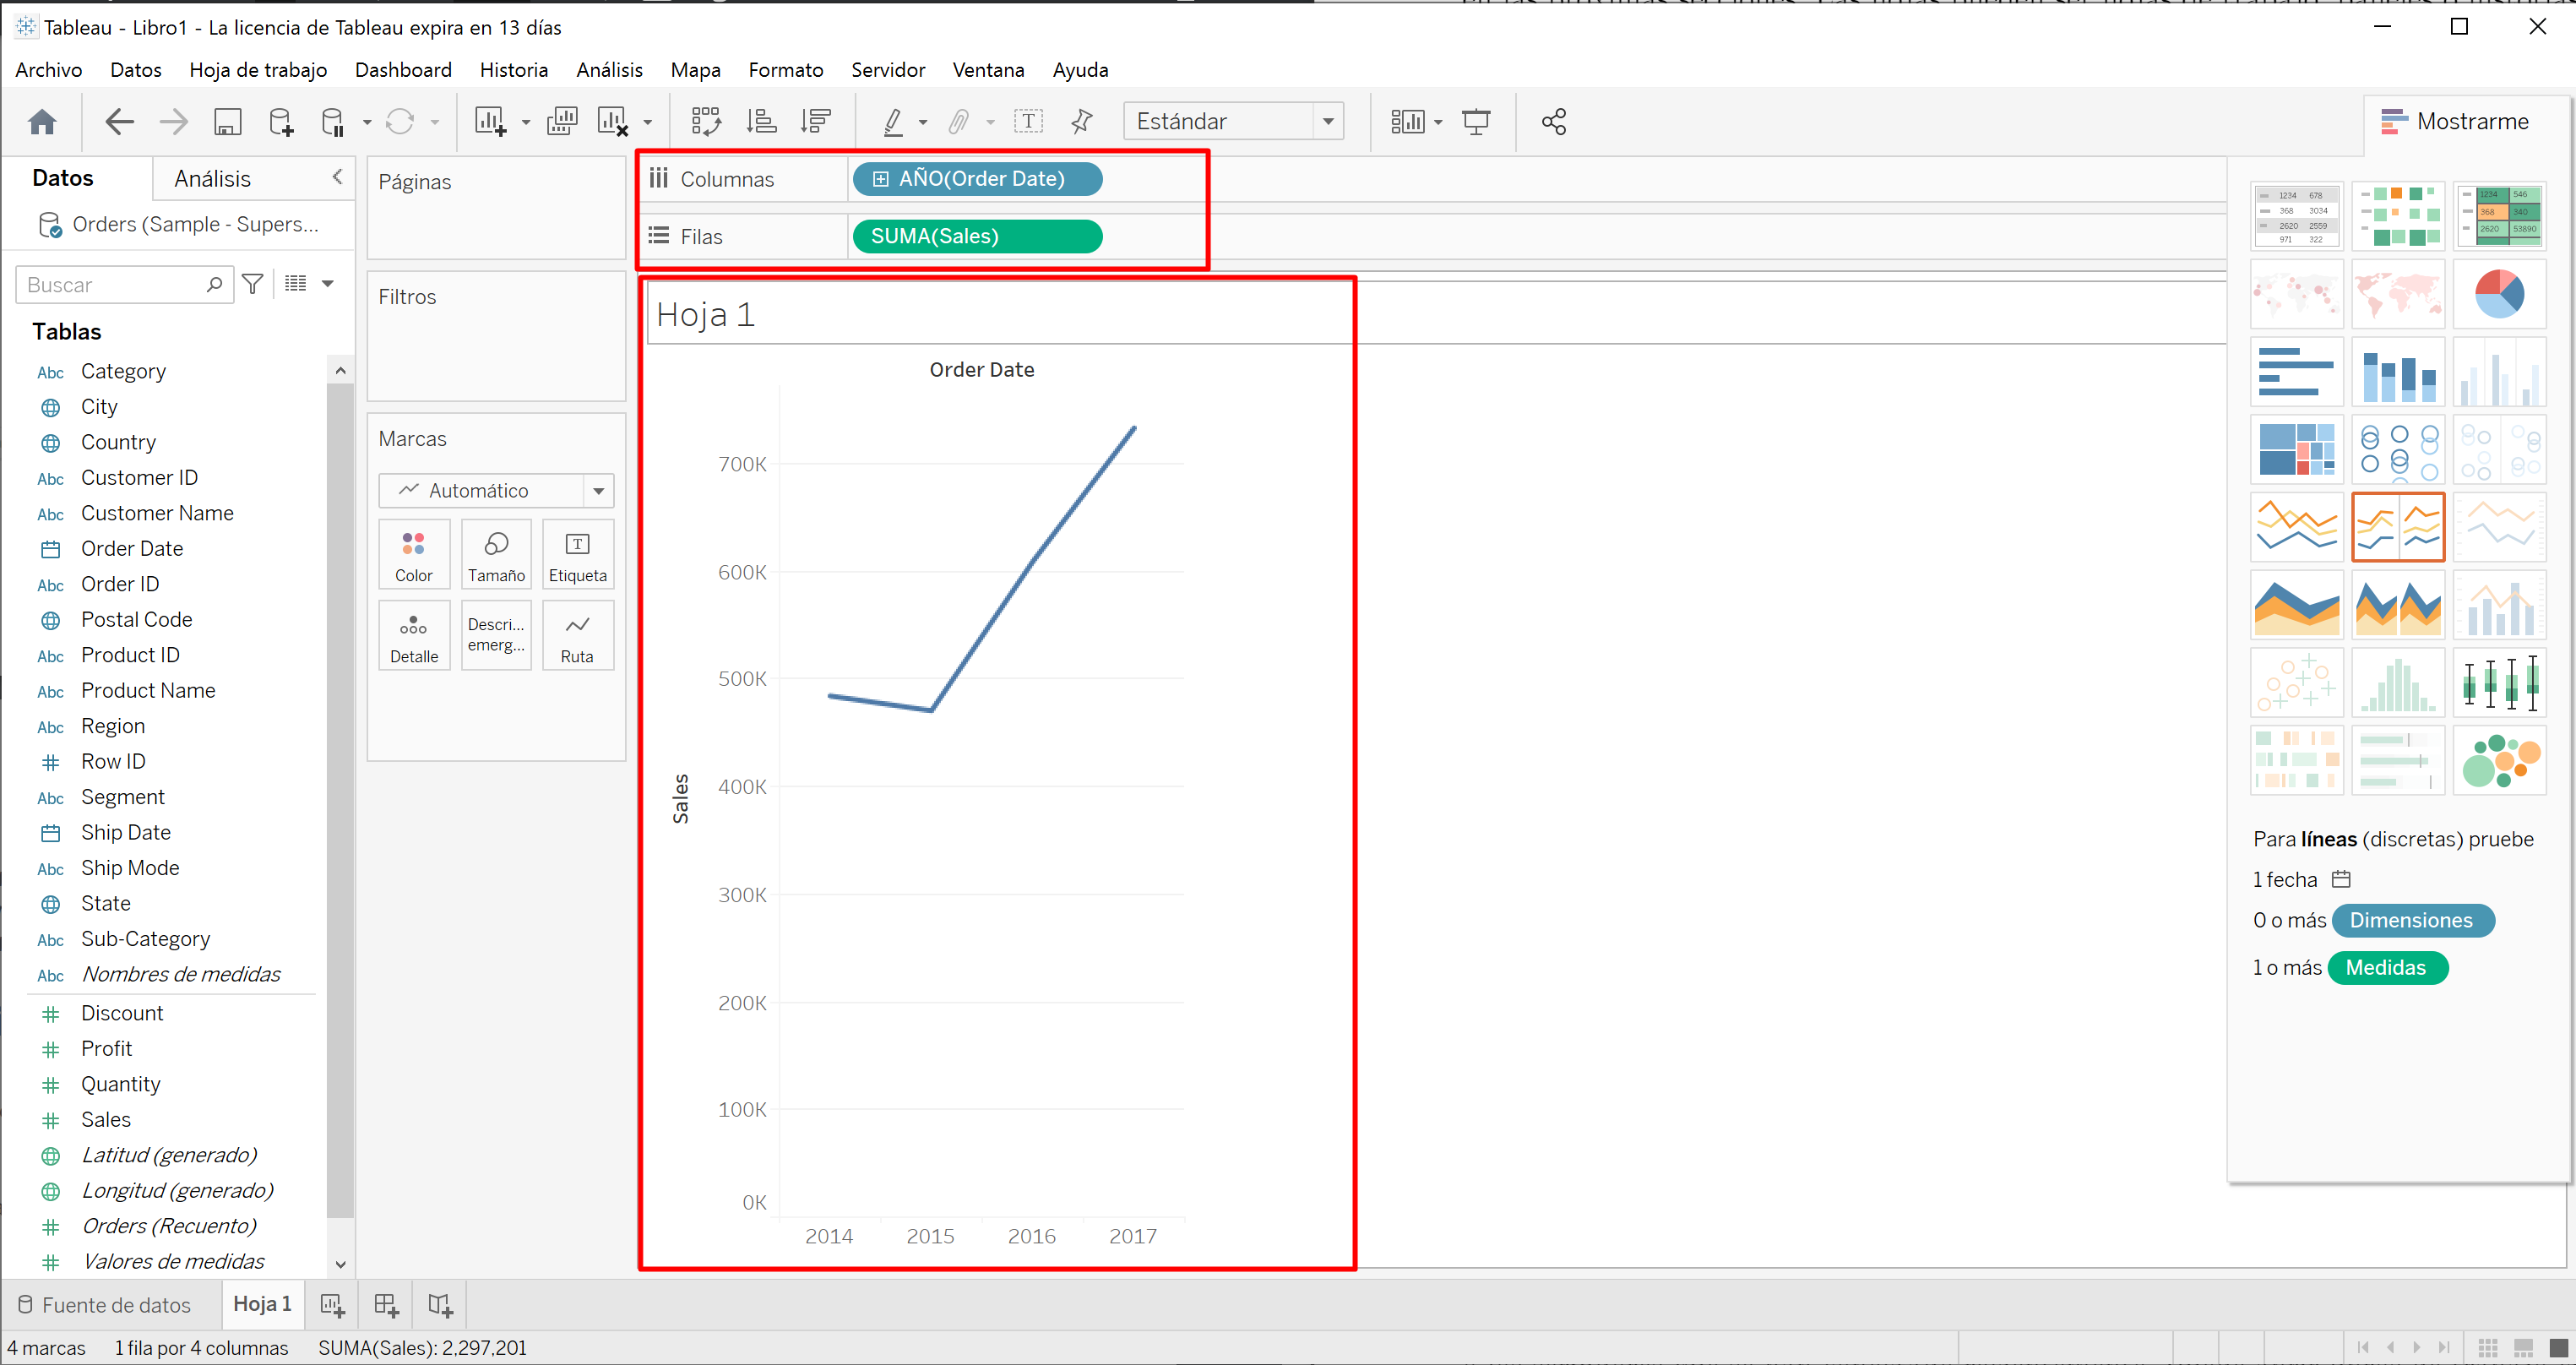
\includegraphics[width=16cm]{img/7.png}  
\end{center}
Tableau completa un gráfico con las ventas agregadas como una suma. Se muestran las ventas totales
agregadas de cada año por fecha de pedido. Tableau siempre completa un gráfico de líneas para una
vista que incluye un campo de tiempo, que en este ejemplo es la fecha del pedido .
\\\\¿Qué transmite el gráfico de líneas anterior? Bueno, muestra que las ventas parecen
bastante prometedoras y parecen estar aumentando con el tiempo. Esta es una
información valiosa, pero apenas dice mucho sobre los productos que contribuyen a
aumentar las ventas. Profundicemos más para obtener más información.

\subsection{Refinando la vista}
Profundicemos e intentemos obtener más información sobre qué productos generan más
ventas. Comencemos agregando las categorías de productos para ver los totales de ventas de una
manera diferente.
\\\\STEPS:
\\\\1. Category está presente en el panel Dimensiones. Arrástrelo al estante de columnas y colóquelo
junto a YEAR(Order Date). El Categorydebe ser colocado a la derecha de Year. Al
hacerlo, la vista cambia inmediatamente a un tipo de gráfico de barras desde una línea. El
gráfico muestra el total Sales de cada Product año.
\\Learn more
\\Para ver información sobre cada punto de datos (es decir, una marca) en la vista, coloque el
cursor sobre una de las barras para revelar una información sobre herramientas. La información
sobre herramientas muestra las ventas totales para esa categoría. Aquí está la información sobre
herramientas para la categoría Suministros de oficina para 2016:
\begin{center}
    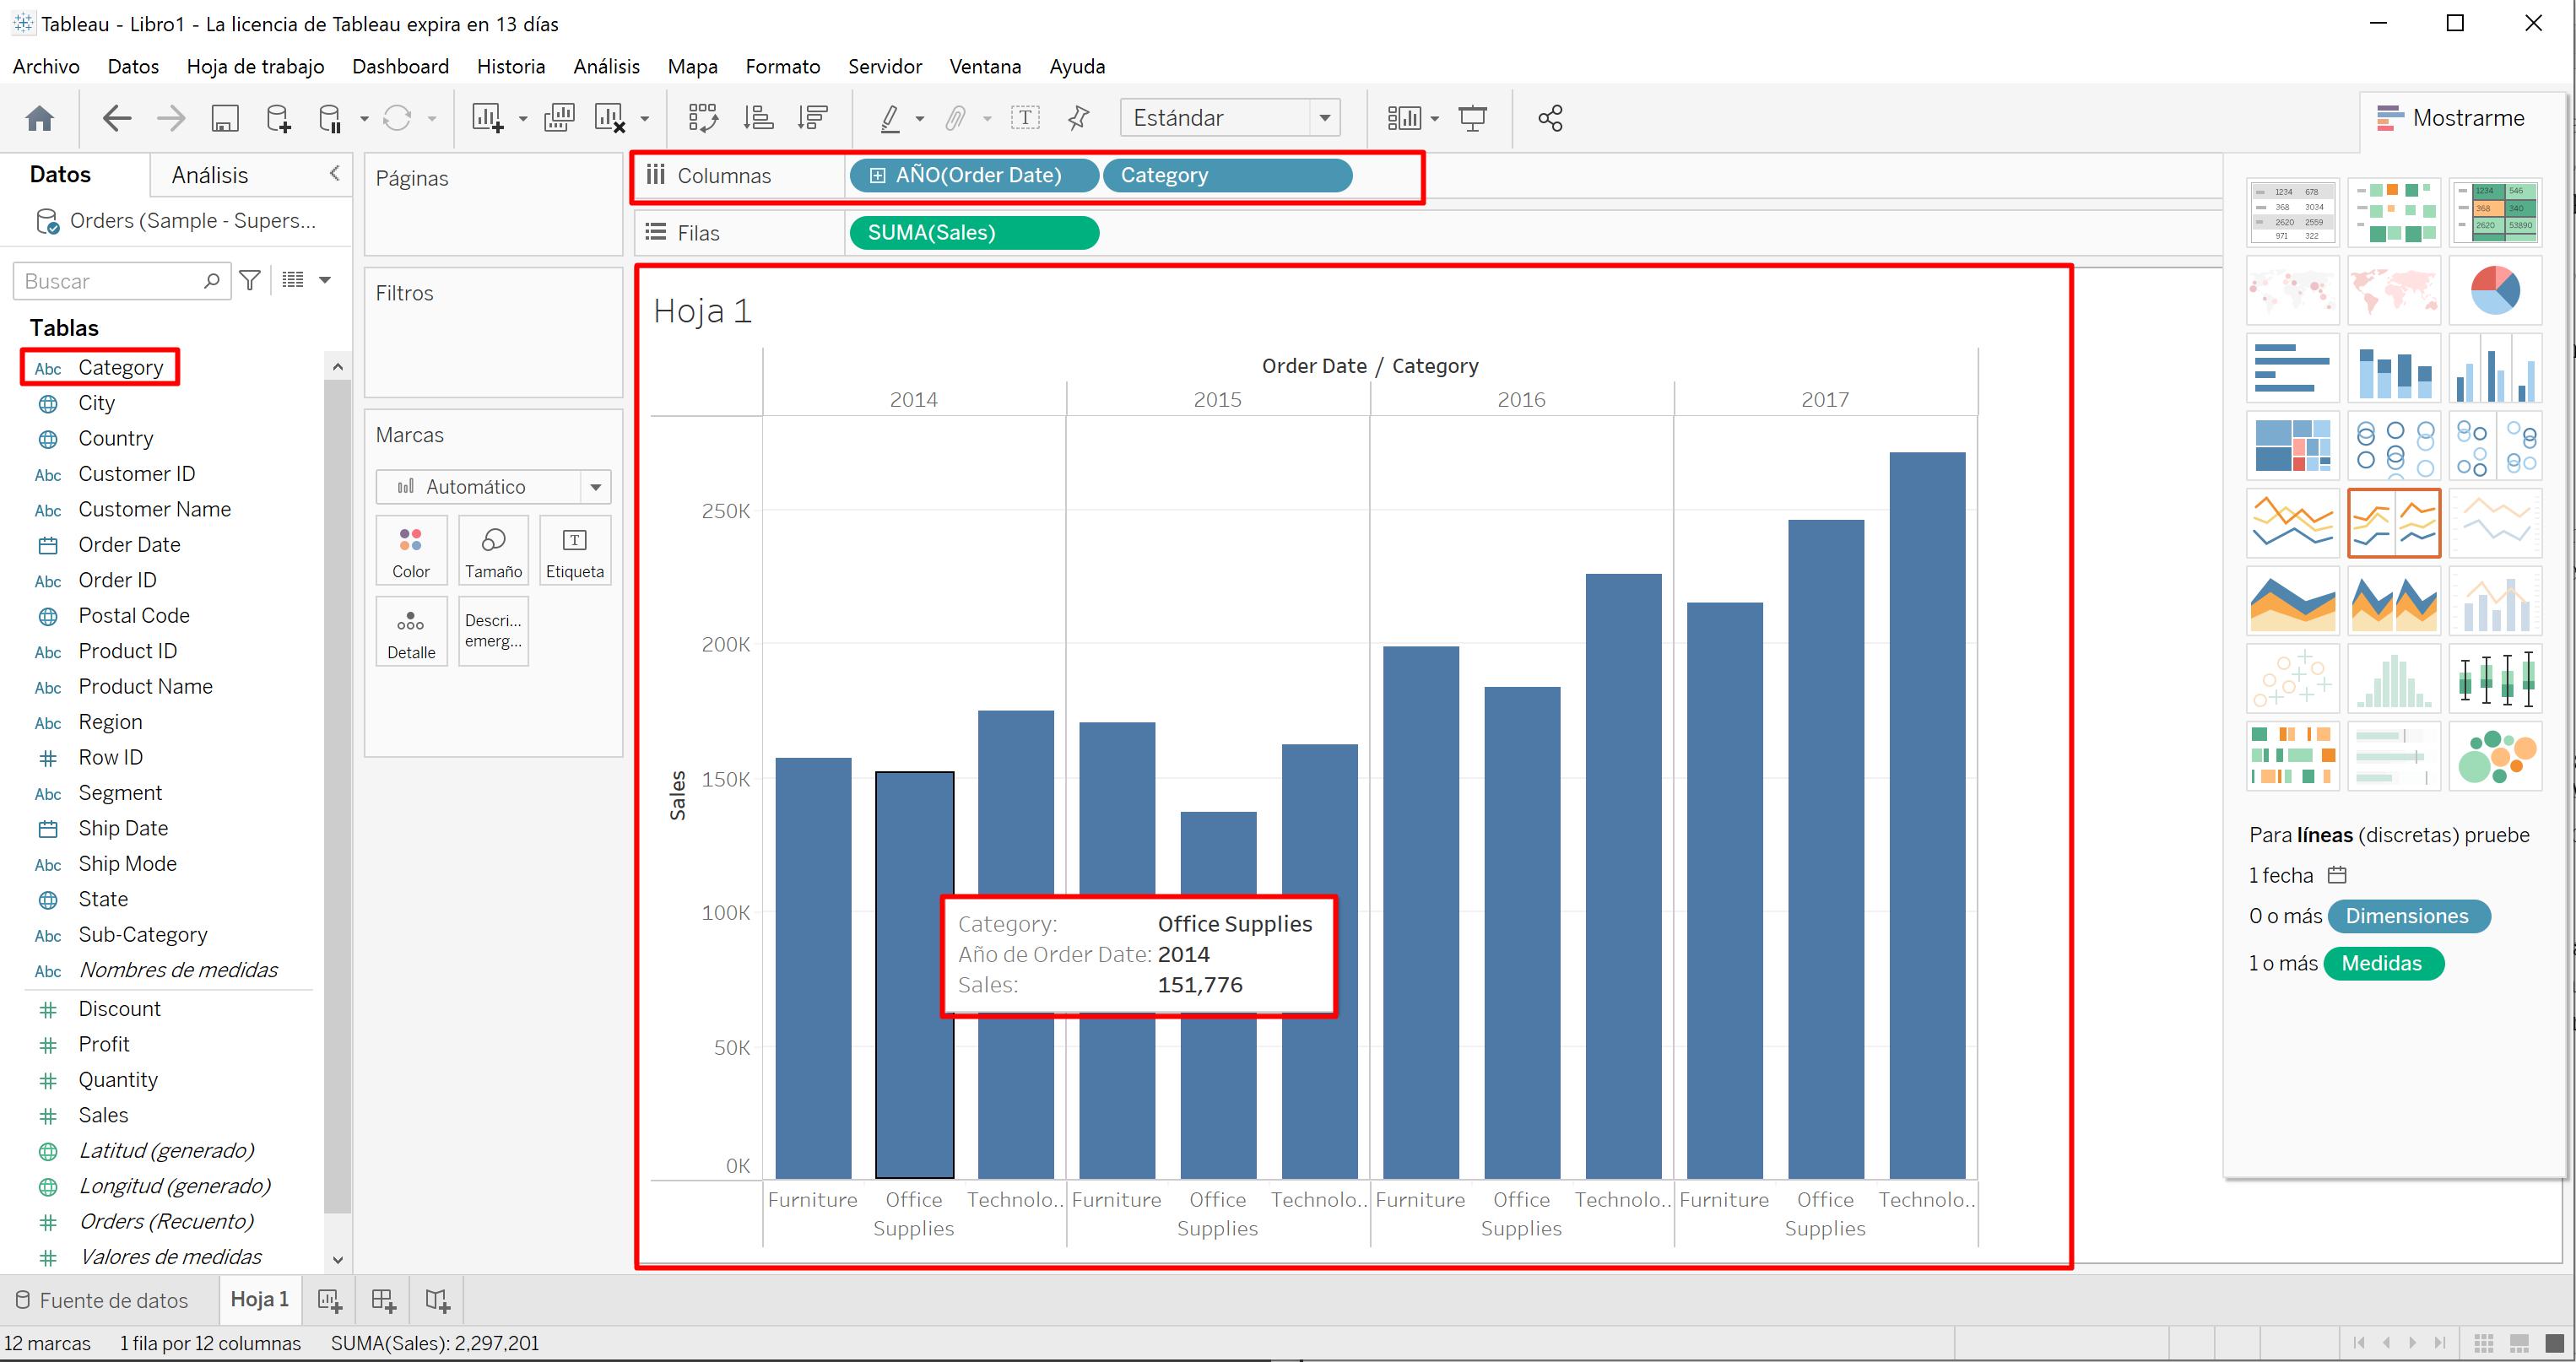
\includegraphics[width=16cm]{img/8.png}  
\end{center}
Para agregar etiquetas a la vista, haga clic Show Mark Labels en en la barra de herramientas.
\begin{center}
    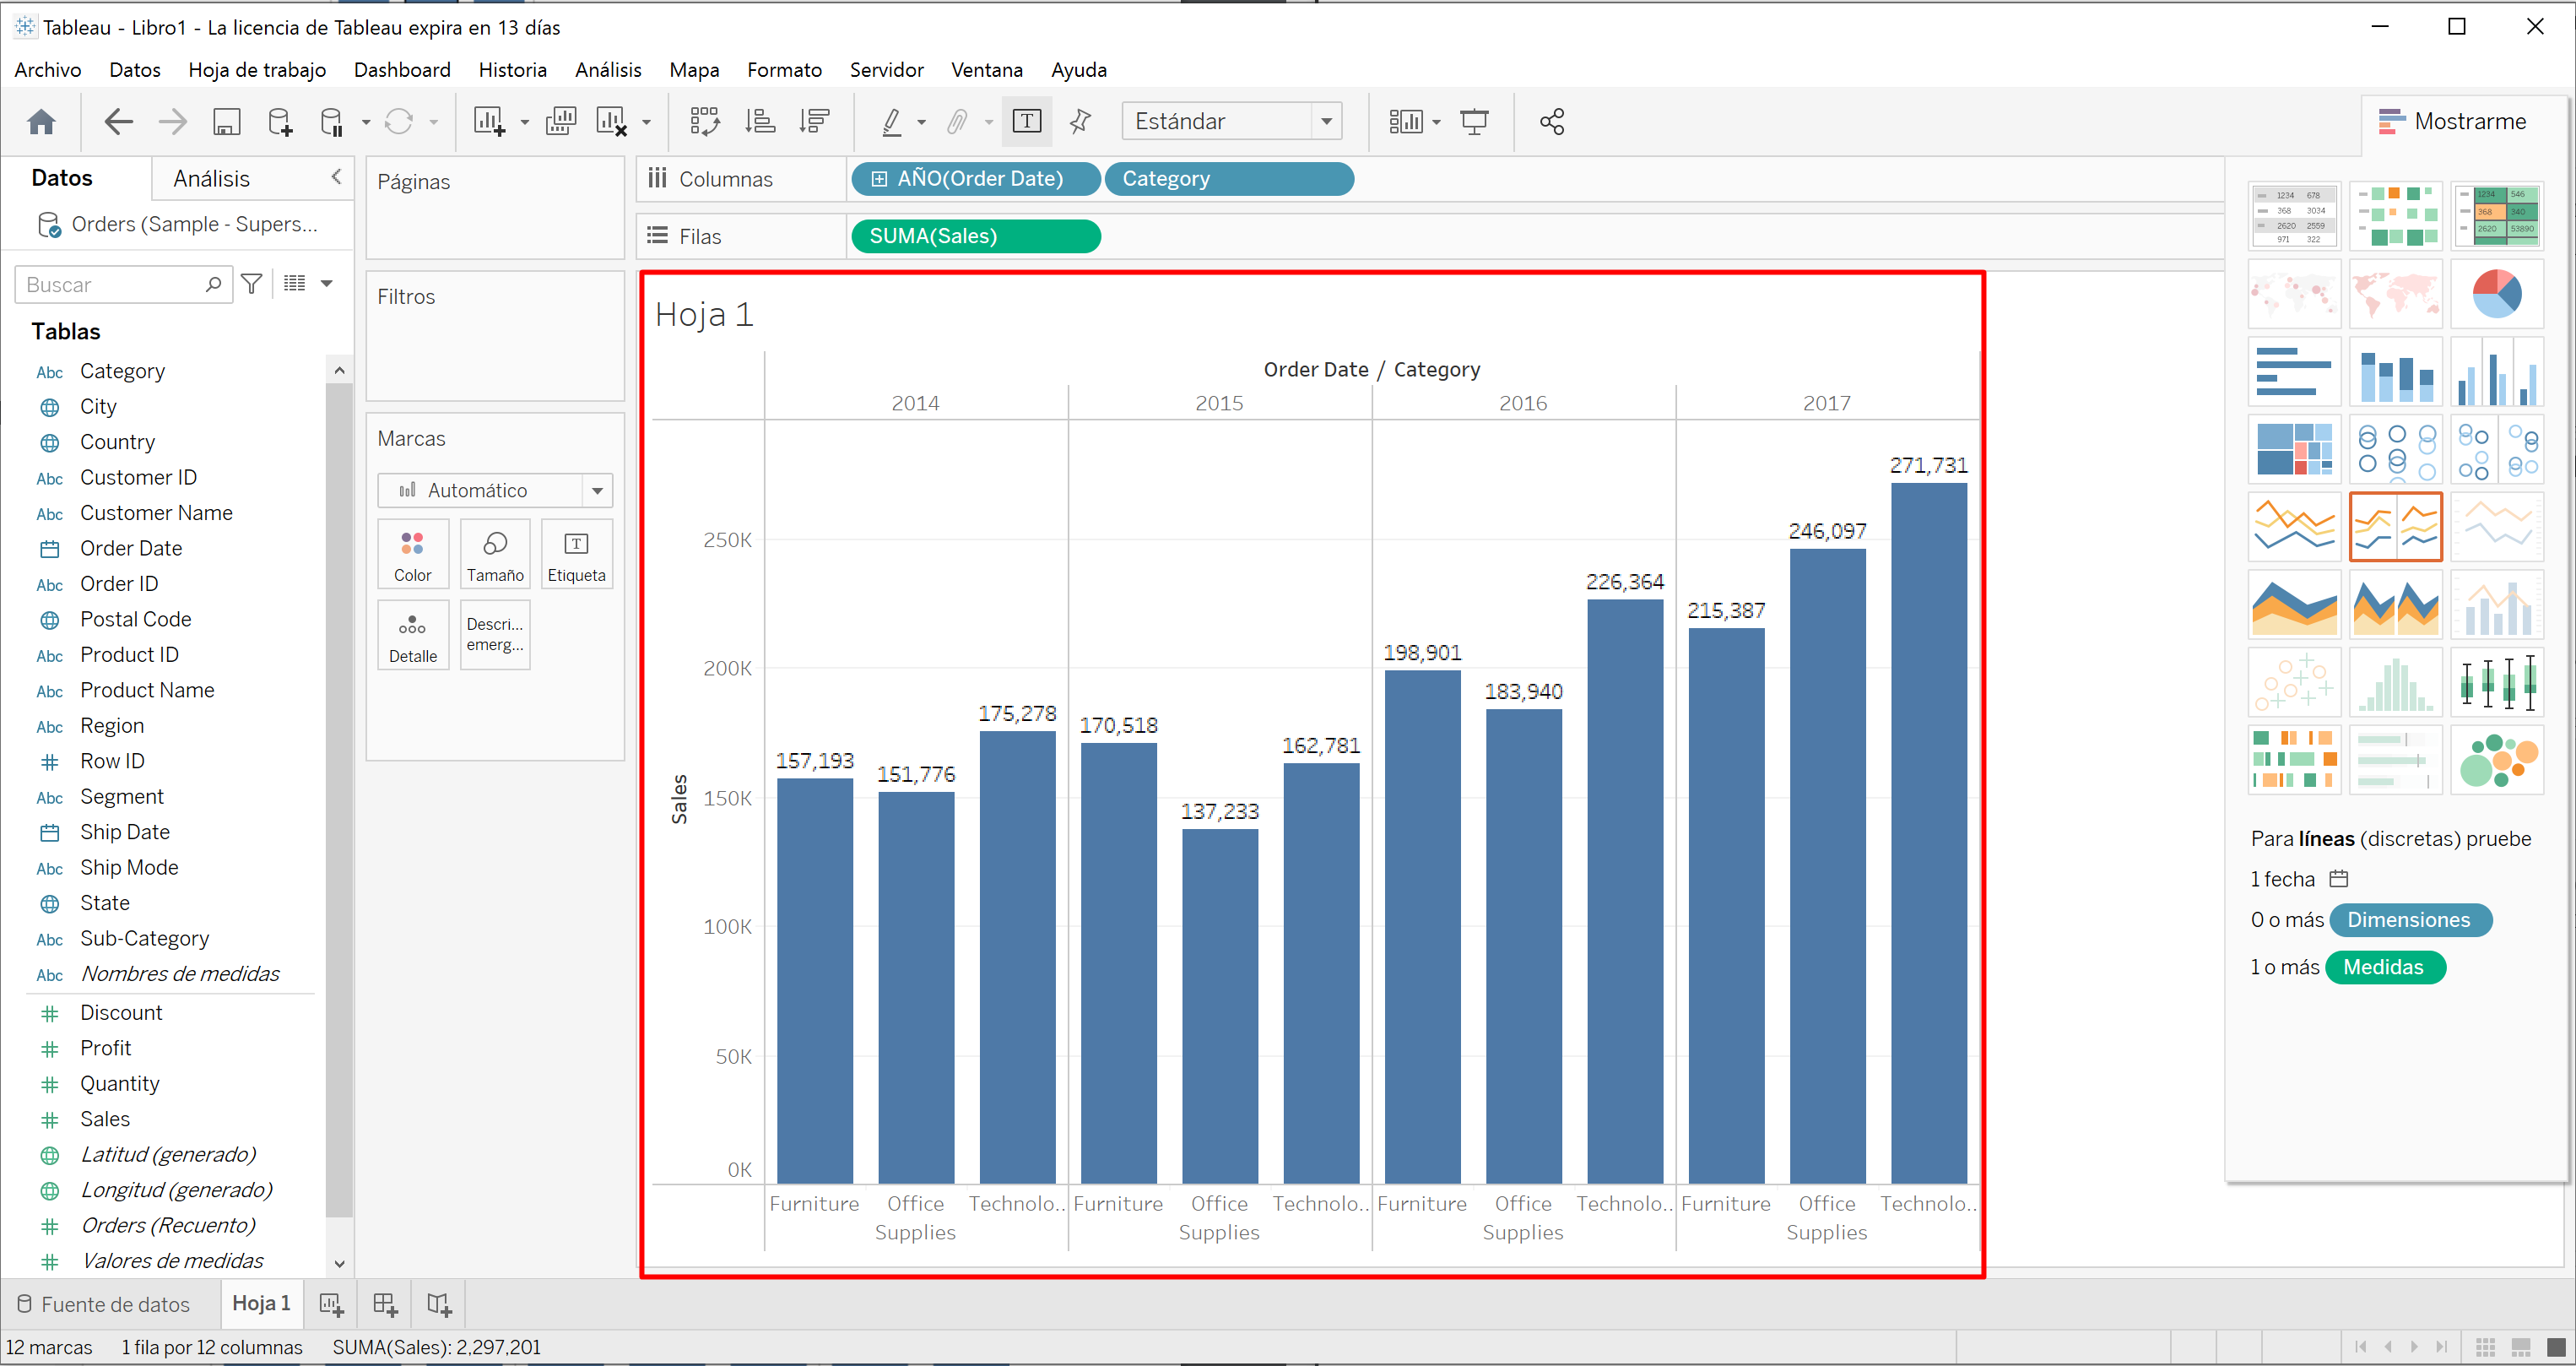
\includegraphics[width=16cm]{img/9.png}  
\end{center}
El gráfico de barras también se puede mostrar horizontalmente en lugar de verticalmente. Haga
clic Swapen la barra de herramientas para el mismo.
\begin{center}
    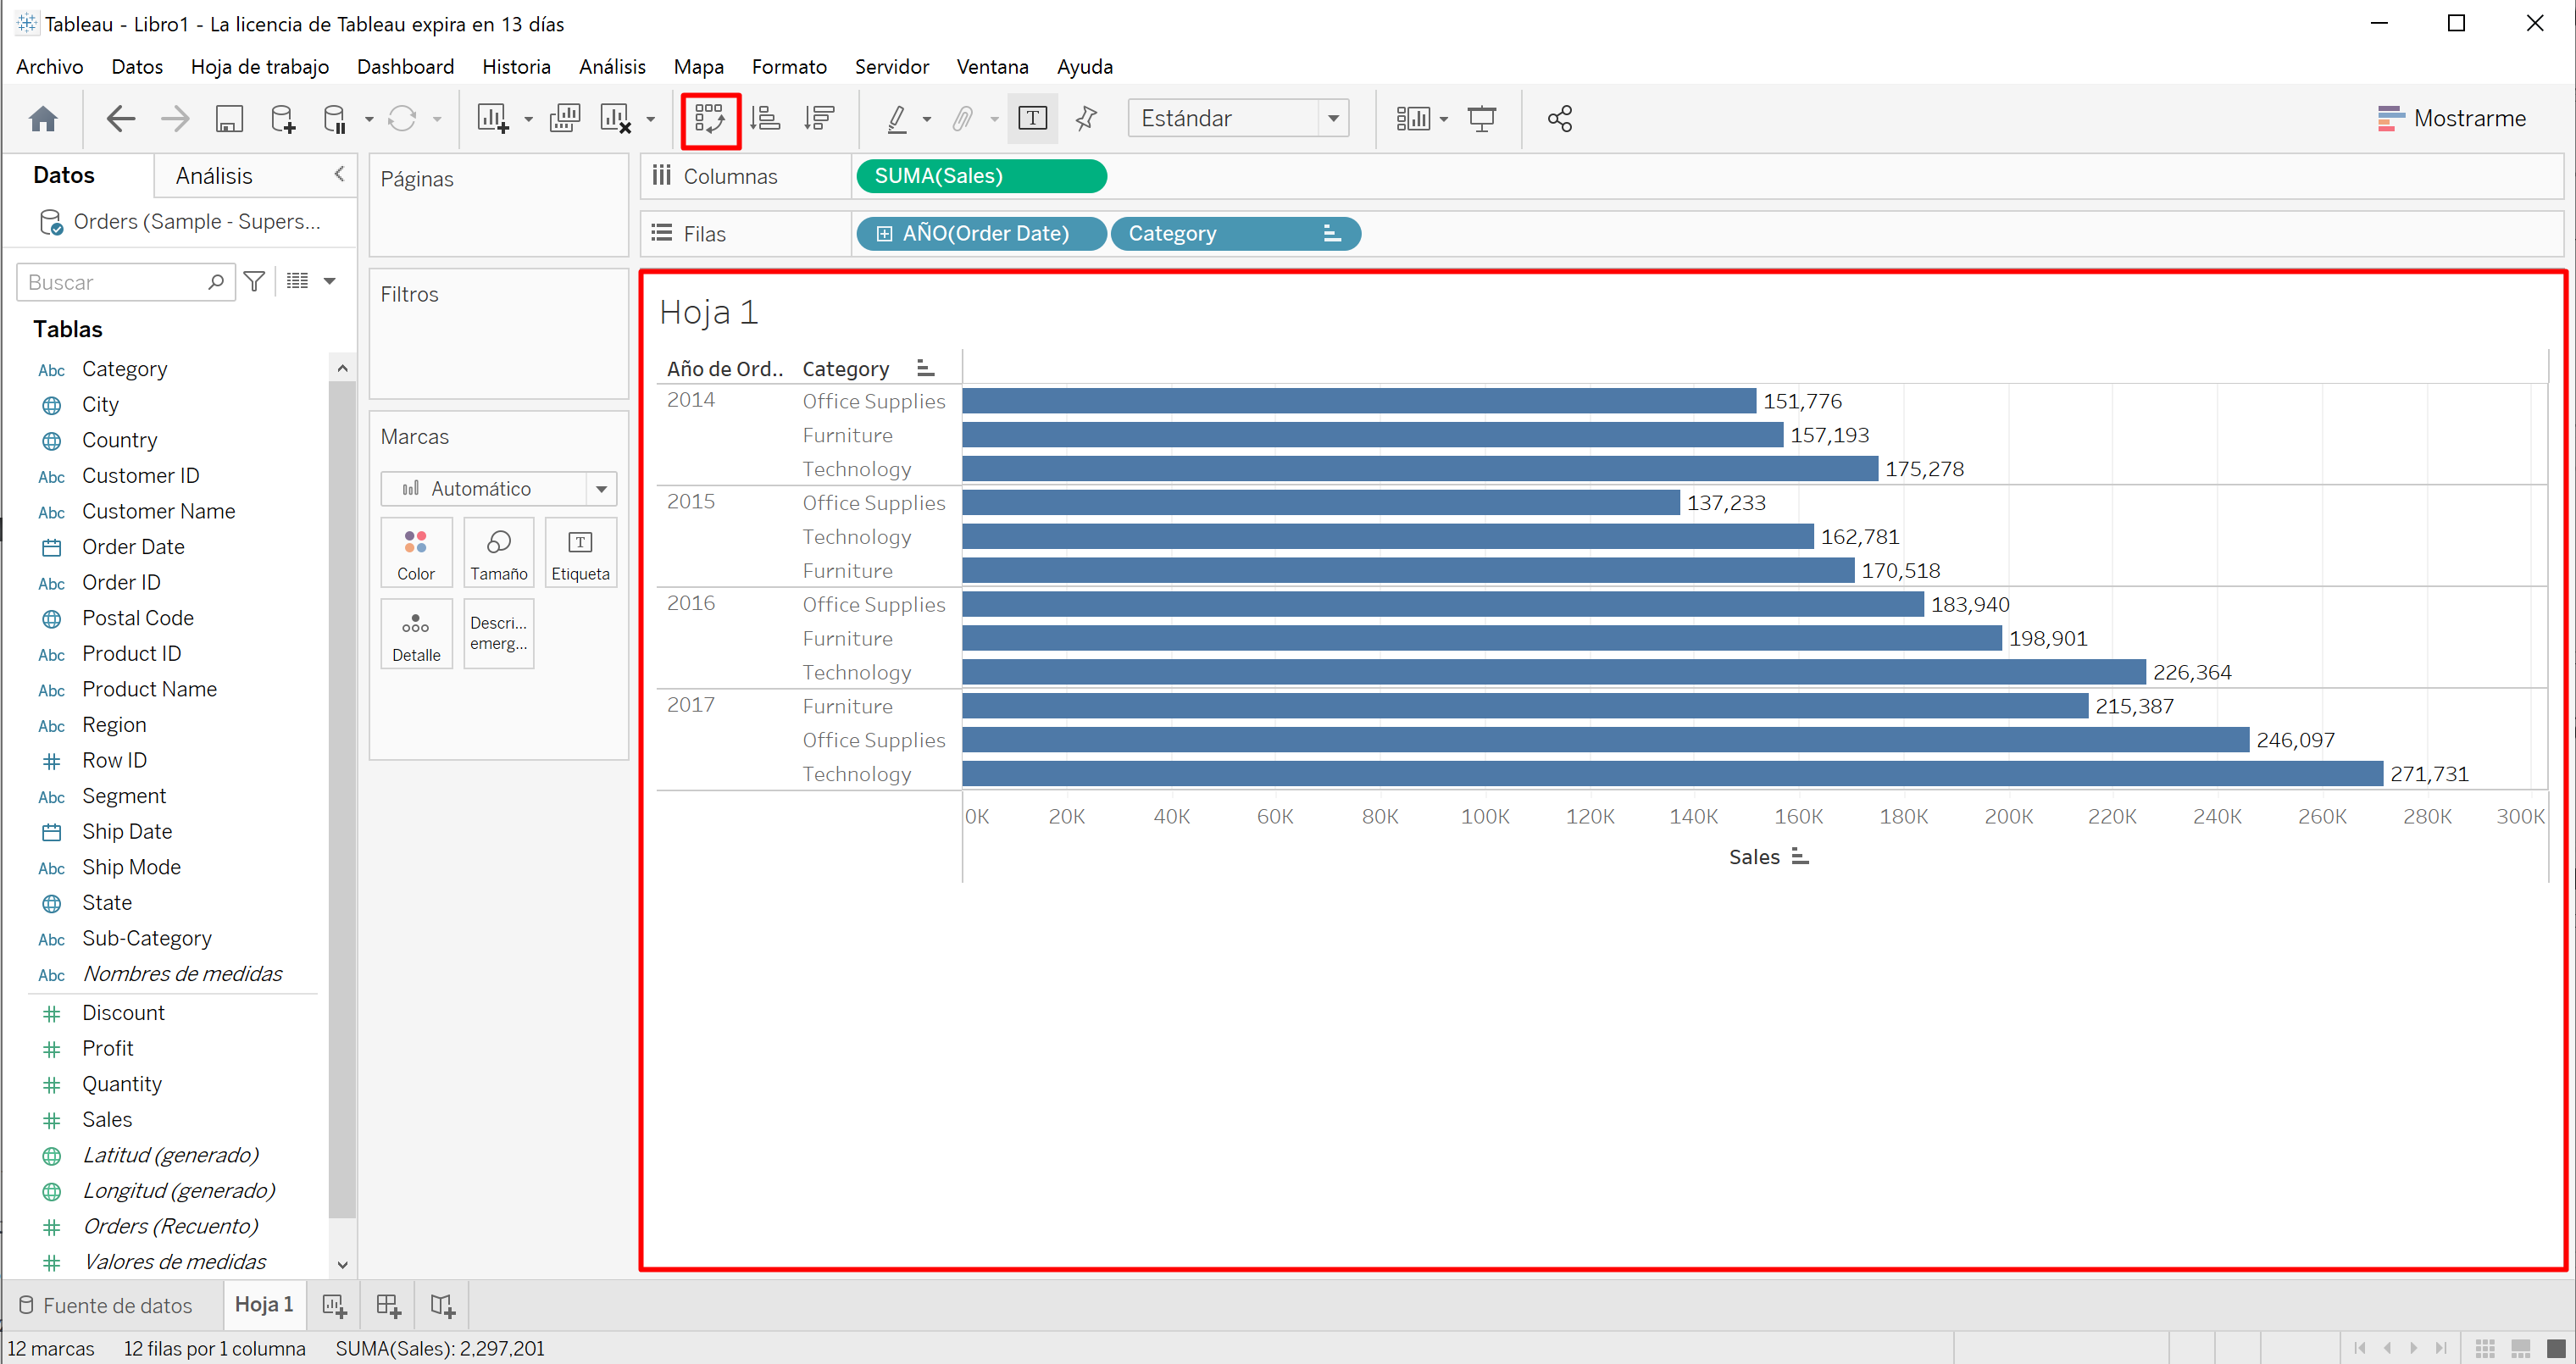
\includegraphics[width=16cm]{img/10.png}  
\end{center}
2. La vista por encima de Niza los espectáculos sales de category, por ejemplo, muebles, equipos
de oficina, y la tecnología. También podemos inferir que las ventas de muebles están creciendo más
rápido que las ventas de suministros de oficina, excepto en 2016. Por lo tanto, sería prudente centrar los
esfuerzos de ventas en muebles en lugar de suministros de oficina. Pero los muebles son una categoría
amplia y se componen de muchos elementos diferentes. ¿Cómo podemos identificar qué mueble está
contribuyendo a las ventas máximas?
\\\\Para ayudarnos a responder esa pregunta, decidimos mirar los productos Sub-category para ver
cuáles son los más vendidos. Digamos para la categoría Mobiliario ; queremos ver los detalles
únicamente sobre estanterías, sillas, muebles y mesas. Haremos doble clic o arrastraremos la SubCategory 
dimensión al estante Columnas.
\\\\La subcategoría es otro campo discreto. Además, analiza Categoryy muestra una barra para cada
uno sub-categorydesglosado por categoría y año. Sin embargo, es una enorme cantidad de datos
para entender visualmente. En la siguiente sección, aprenderemos sobre filtros, colores y otras formas
de hacer que la vista sea más comprensible
\begin{center}
    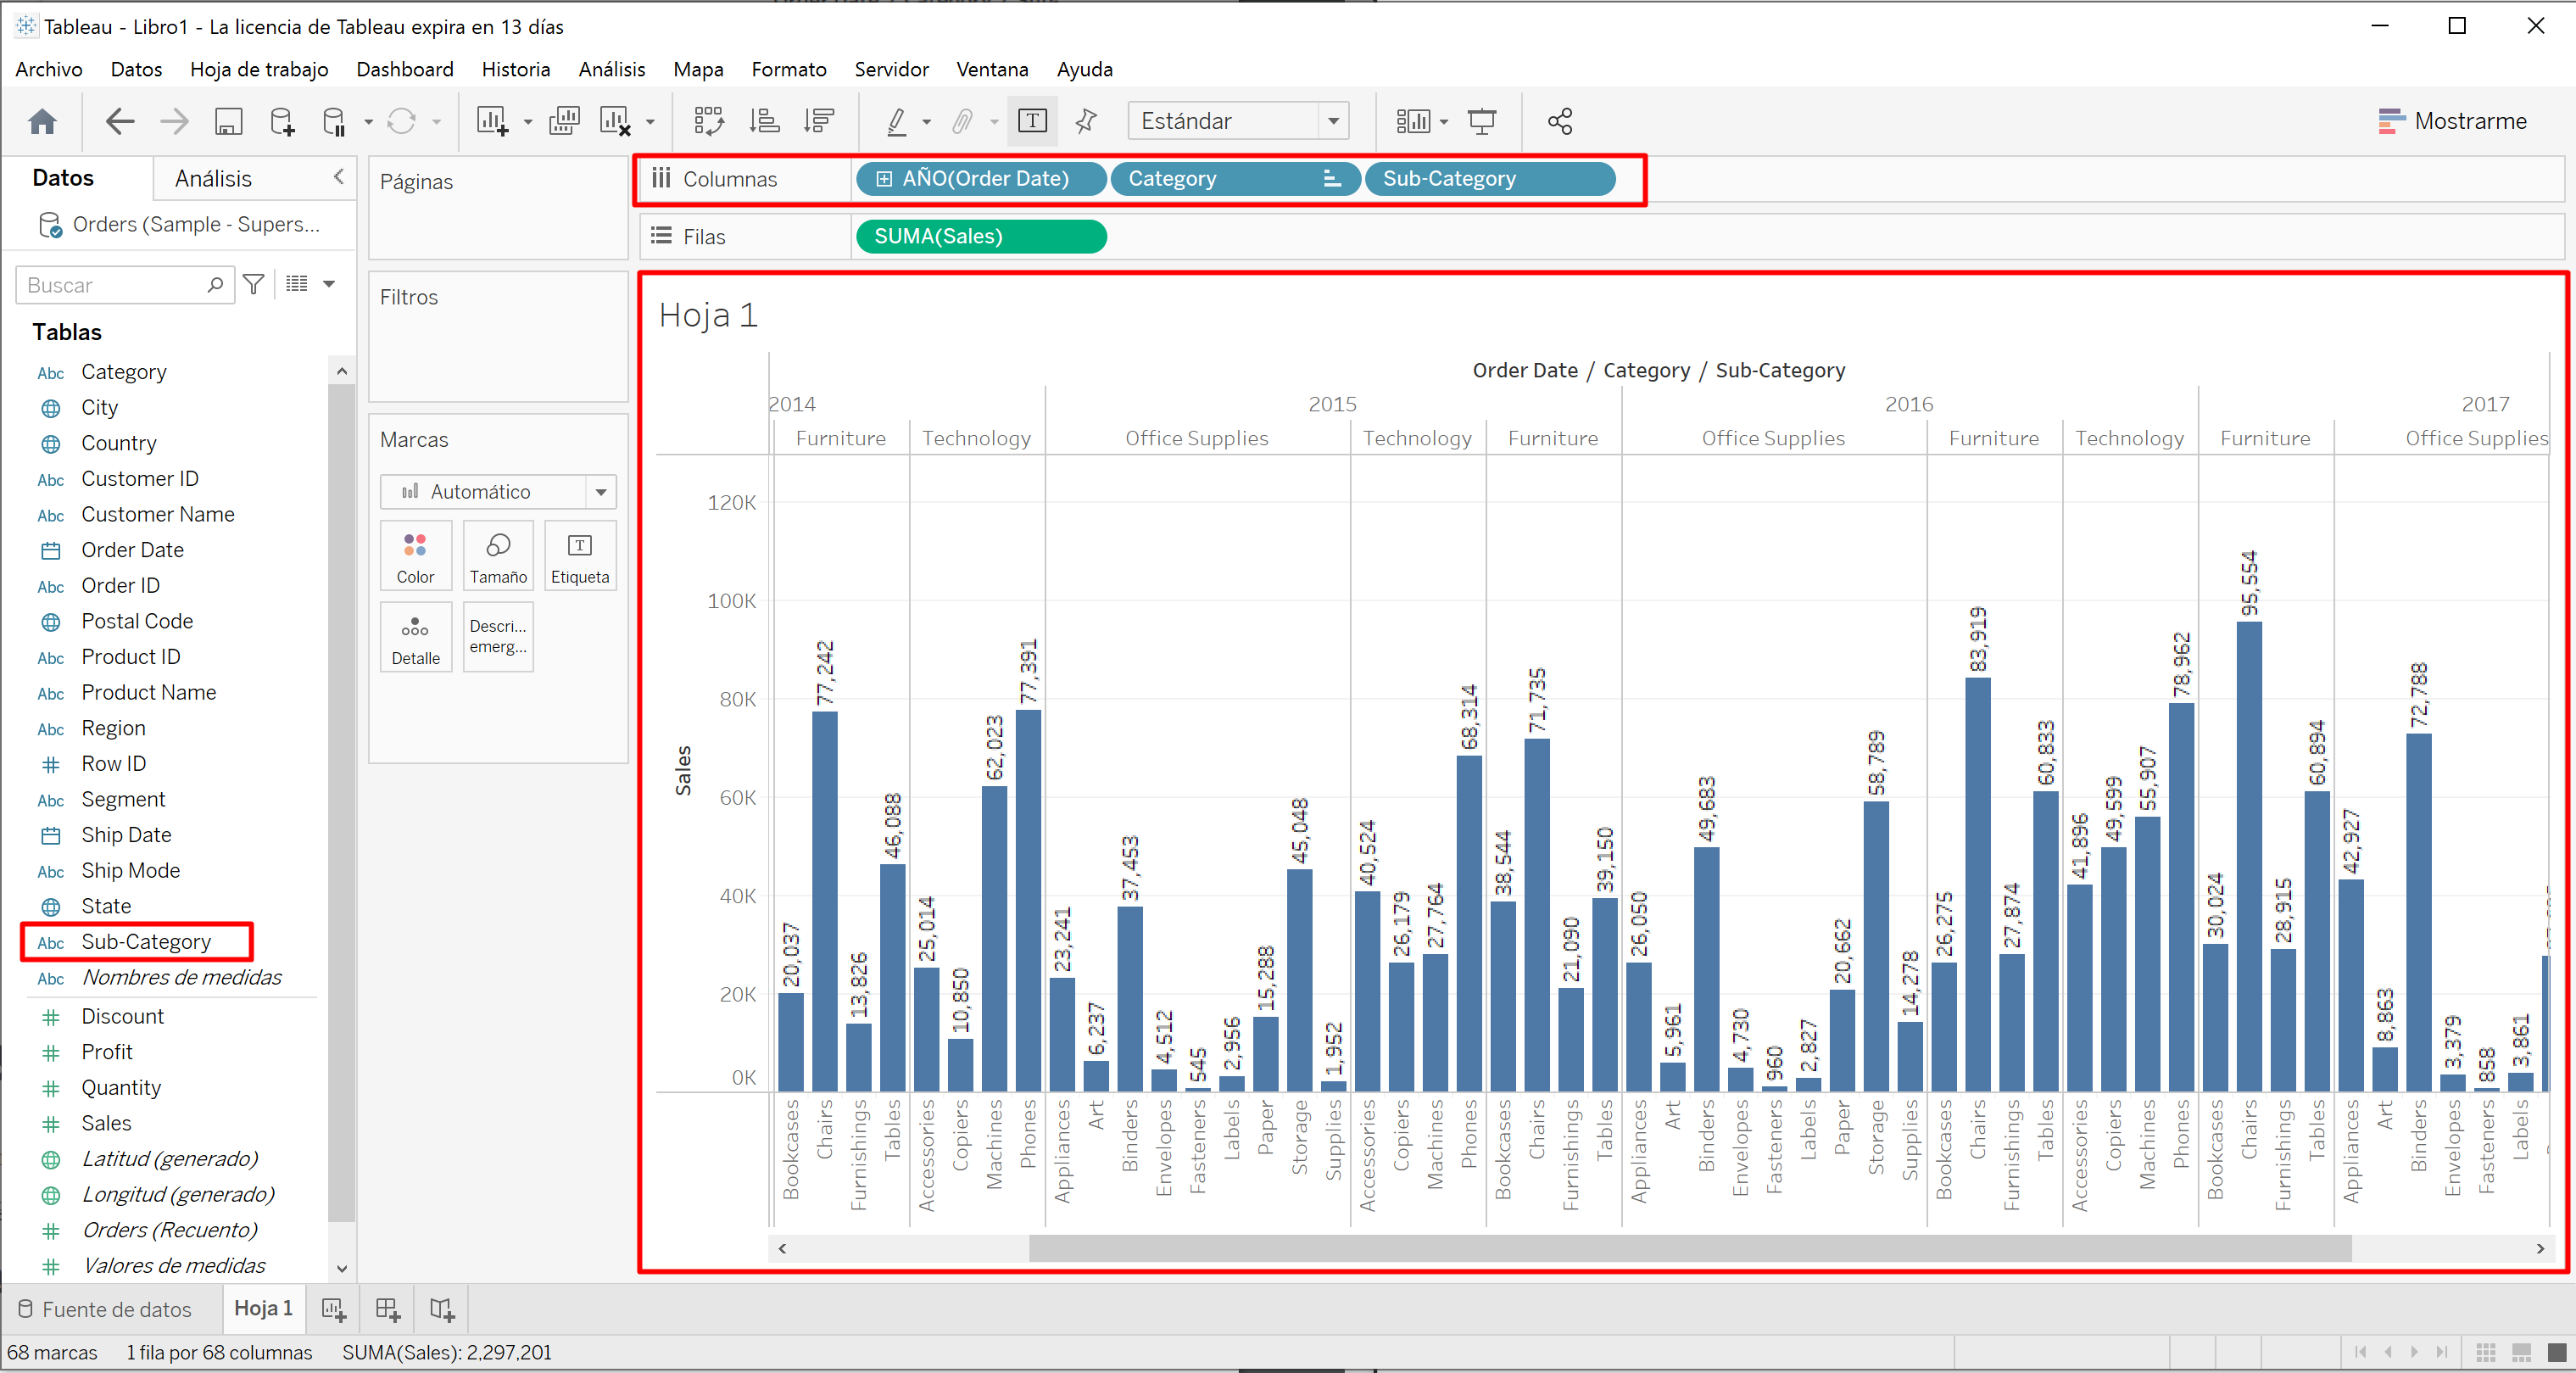
\includegraphics[width=16cm]{img/11.png}  
\end{center}

\section{Enfatizando los resultados} 
En esta sección, intentaremos centrarnos en resultados específicos. Los filtros y colores son formas de
agregar más enfoque a los detalles que nos interesan.
\subsection{Agregar filtros a la vista}
Los filtros se pueden utilizar para incluir o excluir valores en la vista. Aquí intentamos agregar dos
filtros simples a la hoja de trabajo para que sea más fácil ver las ventas de productos por subcategoría
para un año específico.
\\\\STEPS:
\\\\En el panel Datos, en Dimensiones, haga clic con el botón derecho en Fecha de pedido y seleccione
Mostrar filtro. Repita también para el campo Sub-> categoría.
\begin{center}
    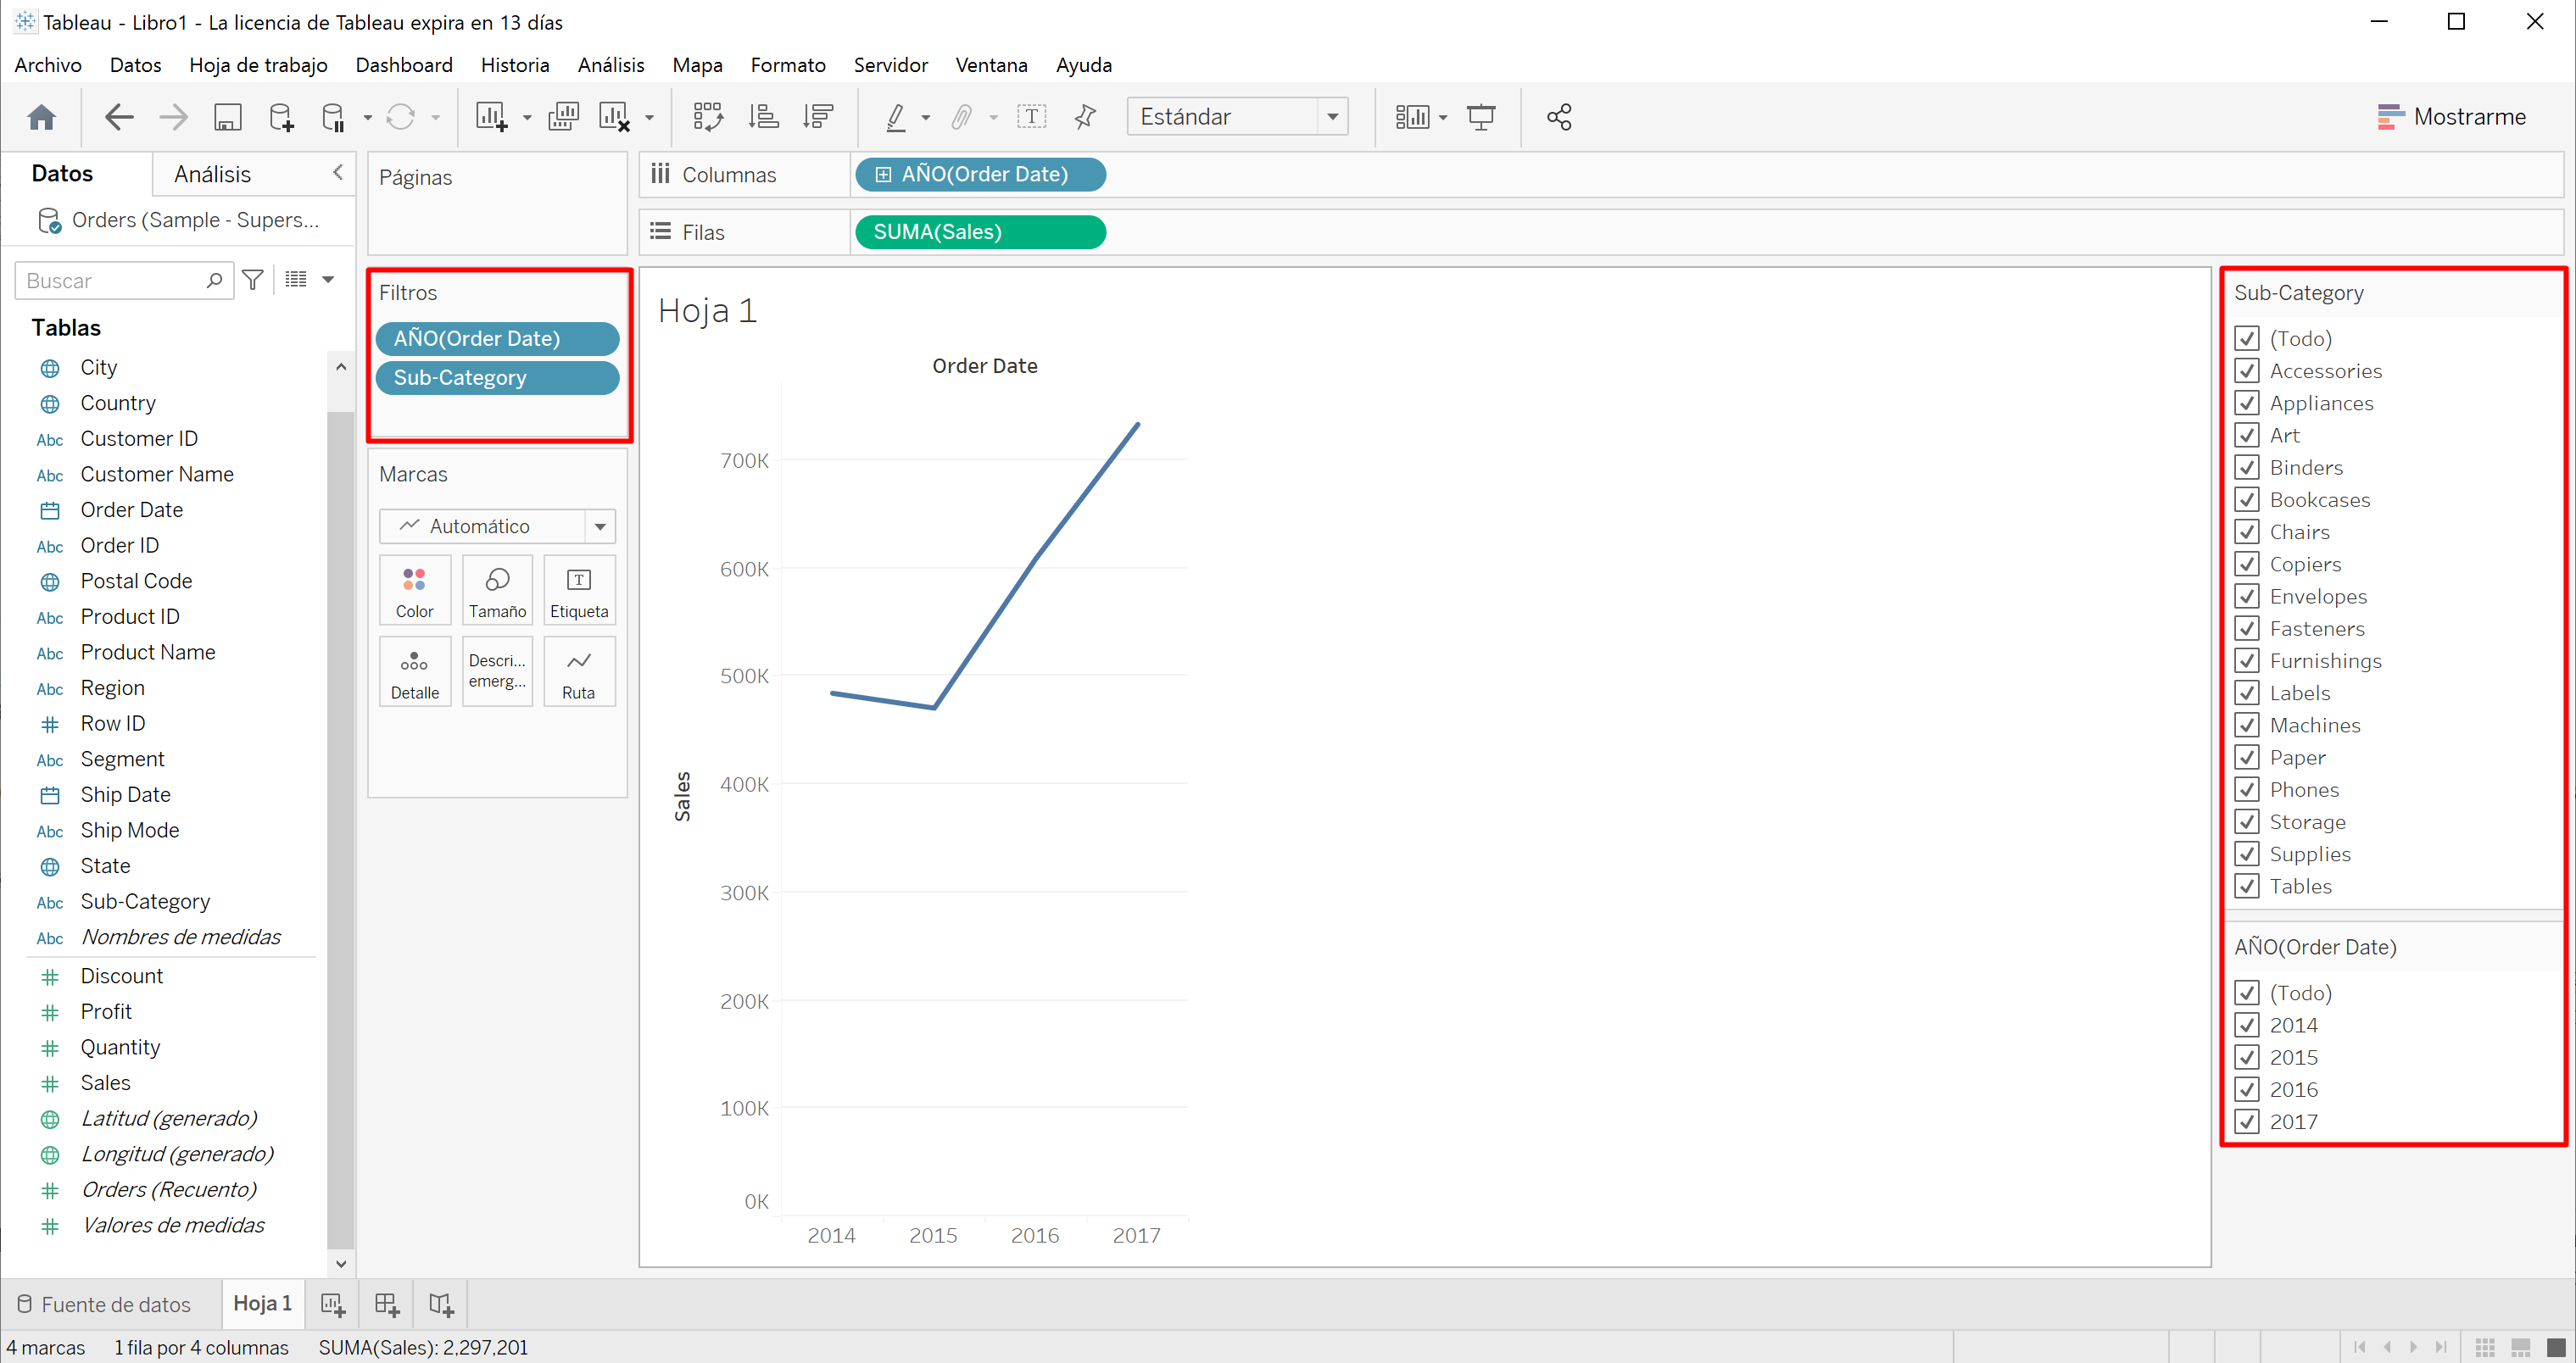
\includegraphics[width=16cm]{img/12.png}  
\end{center}
Los filtros son el tipo de tarjetas y se pueden mover en la hoja de trabajo simplemente
arrastrando y soltando

\subsection{Agregar colores a la vista}
Los colores pueden ser útiles en la identificación visual de un patrón.
\\\\STEPS:
\\\\En el panel Datos, en Medidas, arrastre Beneficio a color en la tarjeta Marcas.
\begin{center}
    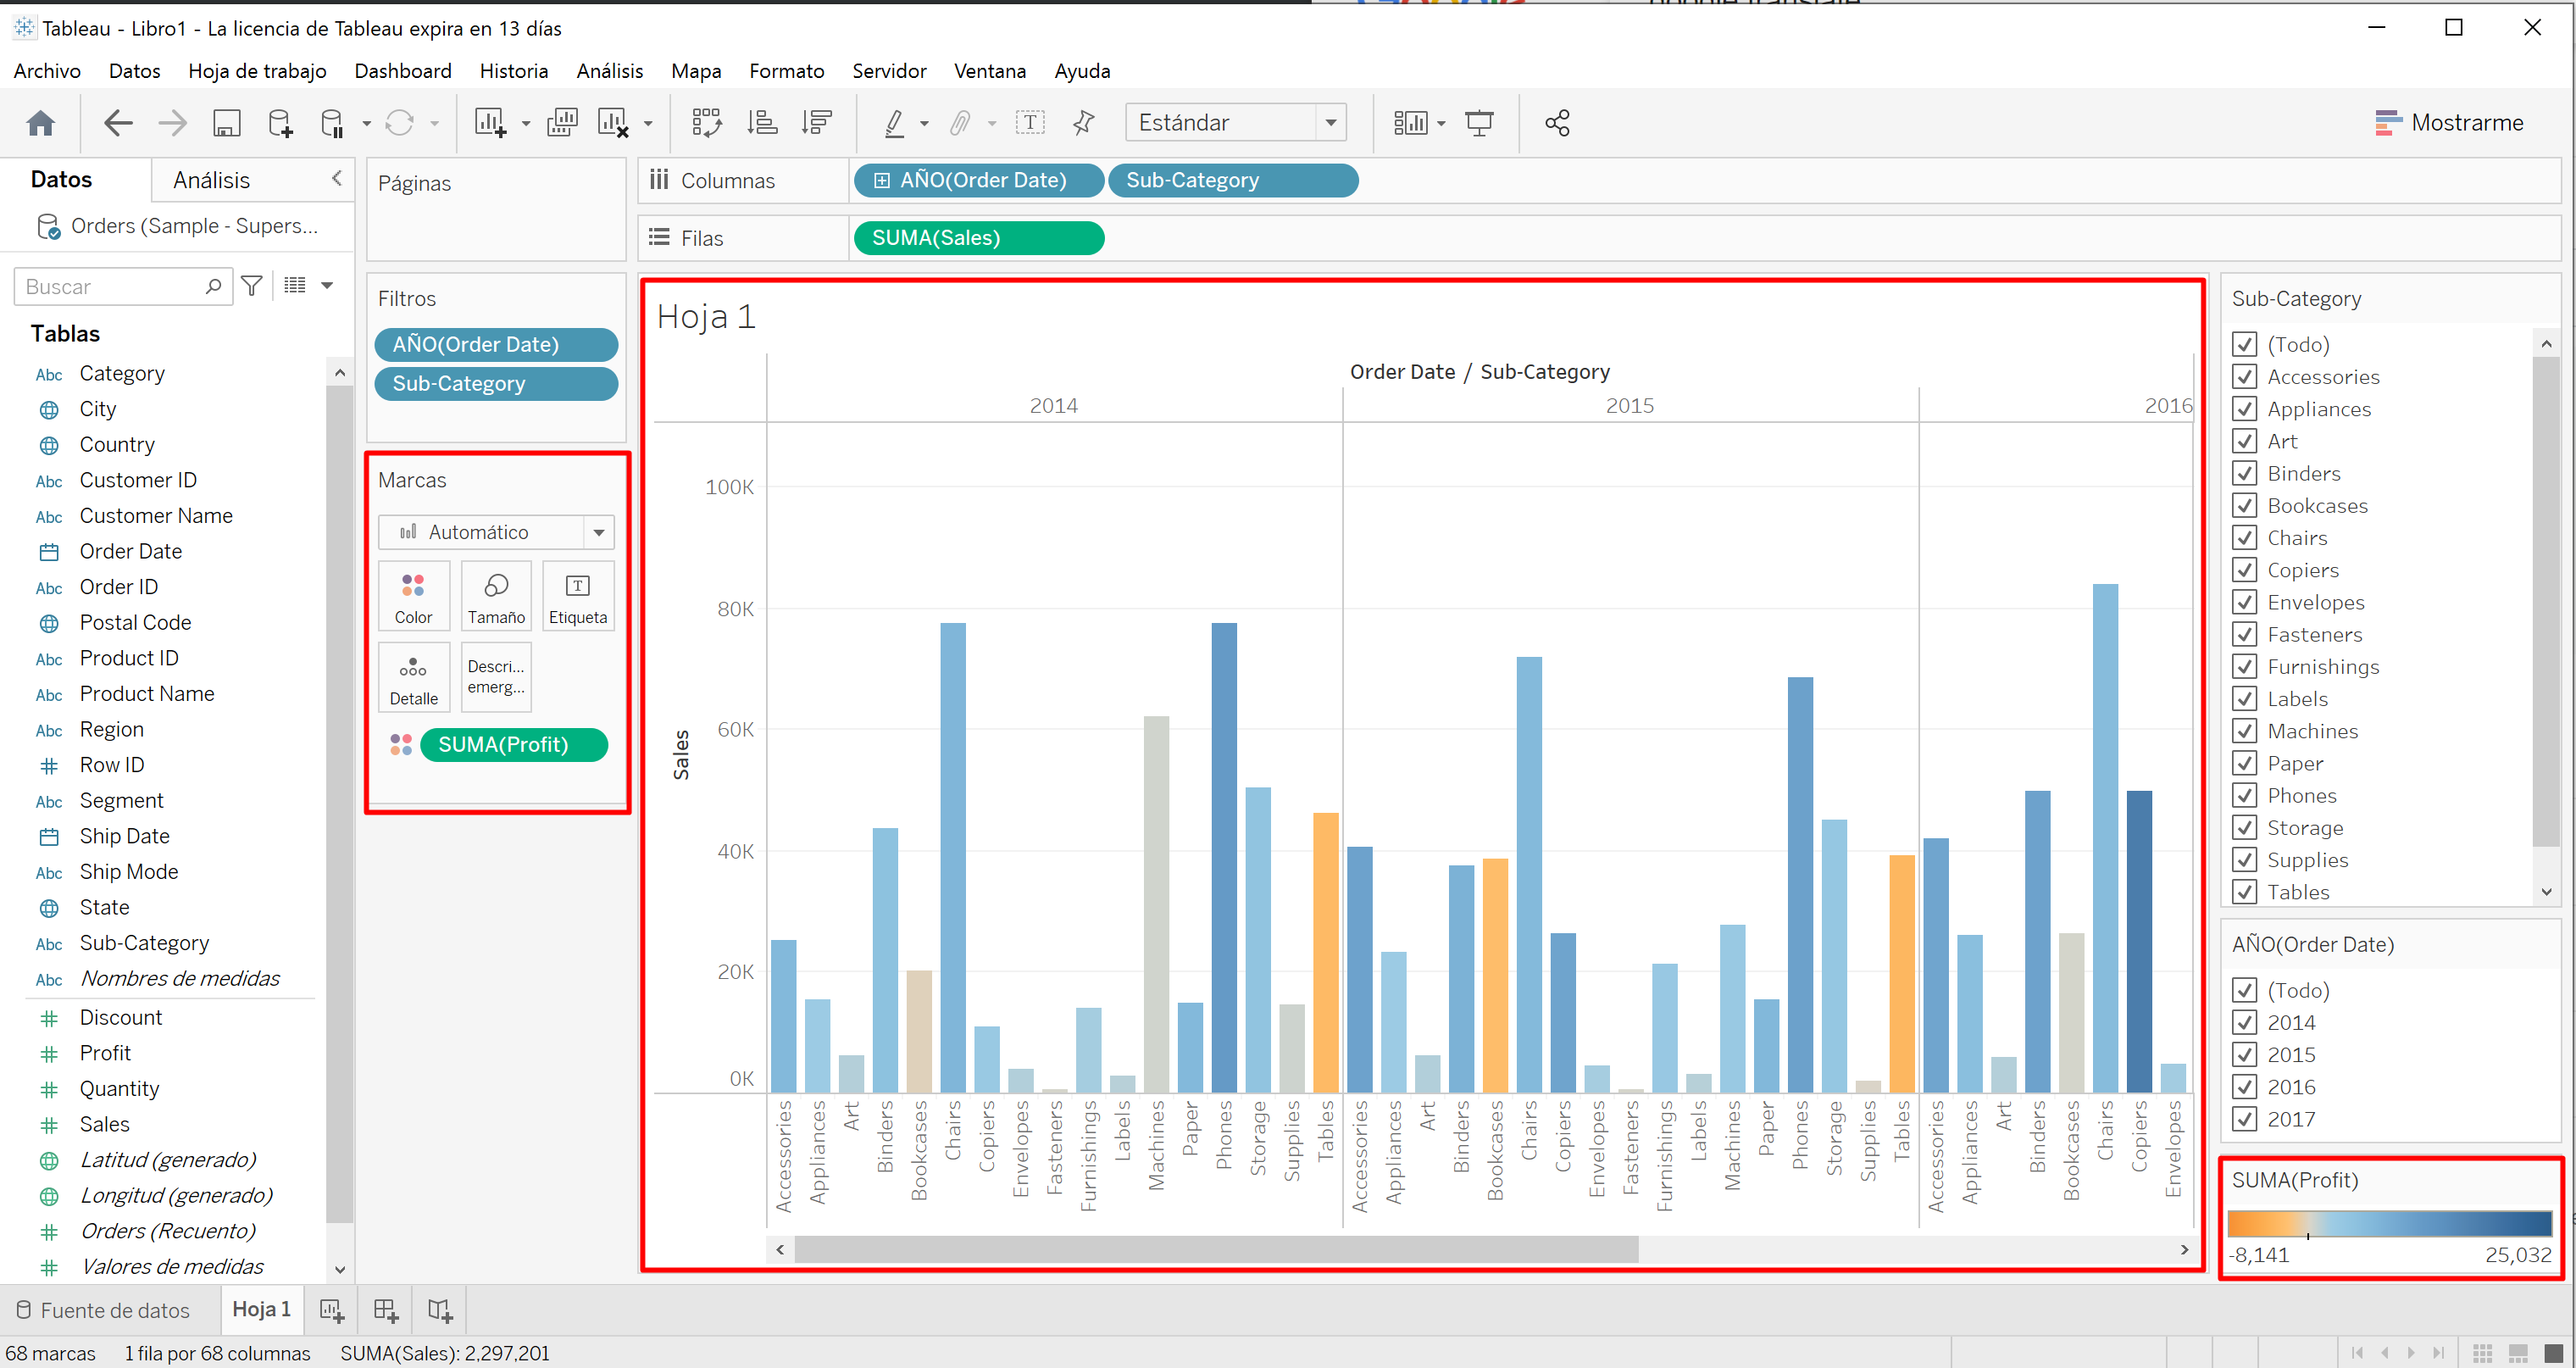
\includegraphics[width=16cm]{img/13.png}  
\end{center}
Se puede ver que las estanterías, las mesas e incluso las máquinas contribuyen a la ganancia
negativa, es decir, a la pérdida. Una visión poderosa.

\subsection{Resultados clave}
Echemos un vistazo más de cerca a los filtros para obtener más información sobre los productos no
rentables.
\\\\STEPS:
\\\\1. En la vista, en la Sub-Category tarjeta de filtro, desactive todas las casillas
excepto Bookcases, Tables, y Machines. Esto saca a la luz un hecho interesante. Mientras
que en algunos años, las librerías y las máquinas fueron realmente rentables. Sin embargo, en
2016, Machines dejó de ser rentable.
\begin{center}
    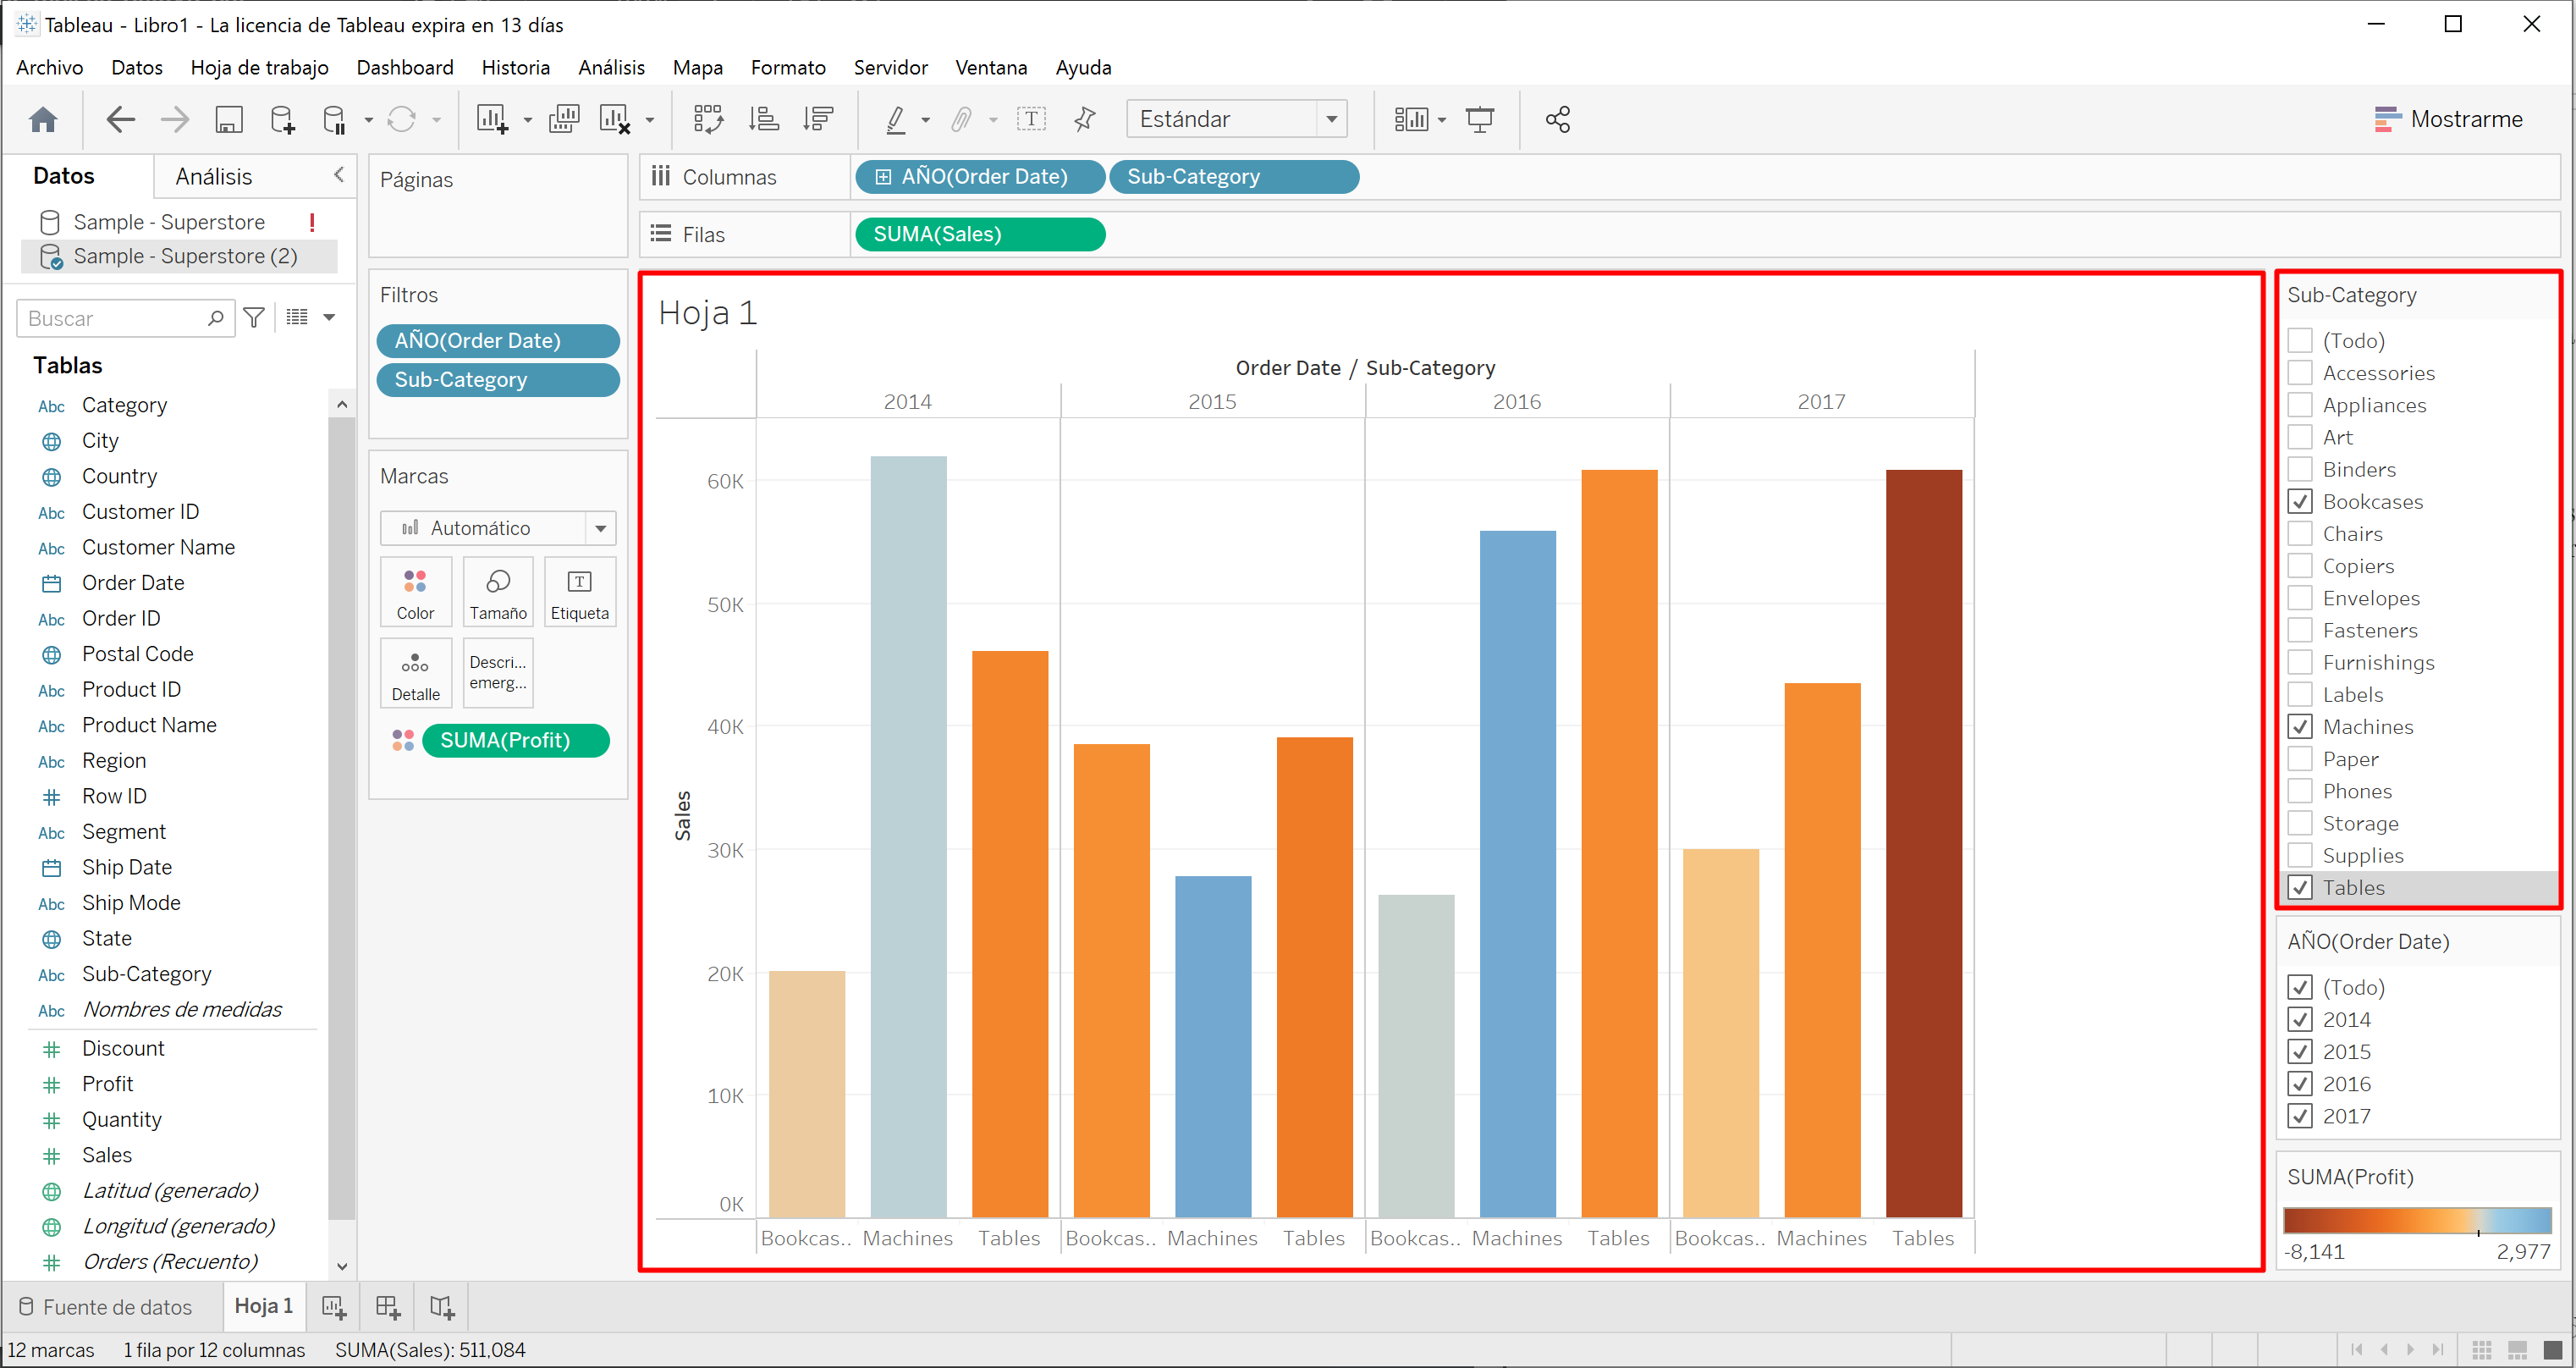
\includegraphics[width=16cm]{img/14.png}  
\end{center}
2. Seleccione All en la Sub-Category tarjeta de filtro para mostrar todas las subcategorías
nuevamente.
\begin{center}
    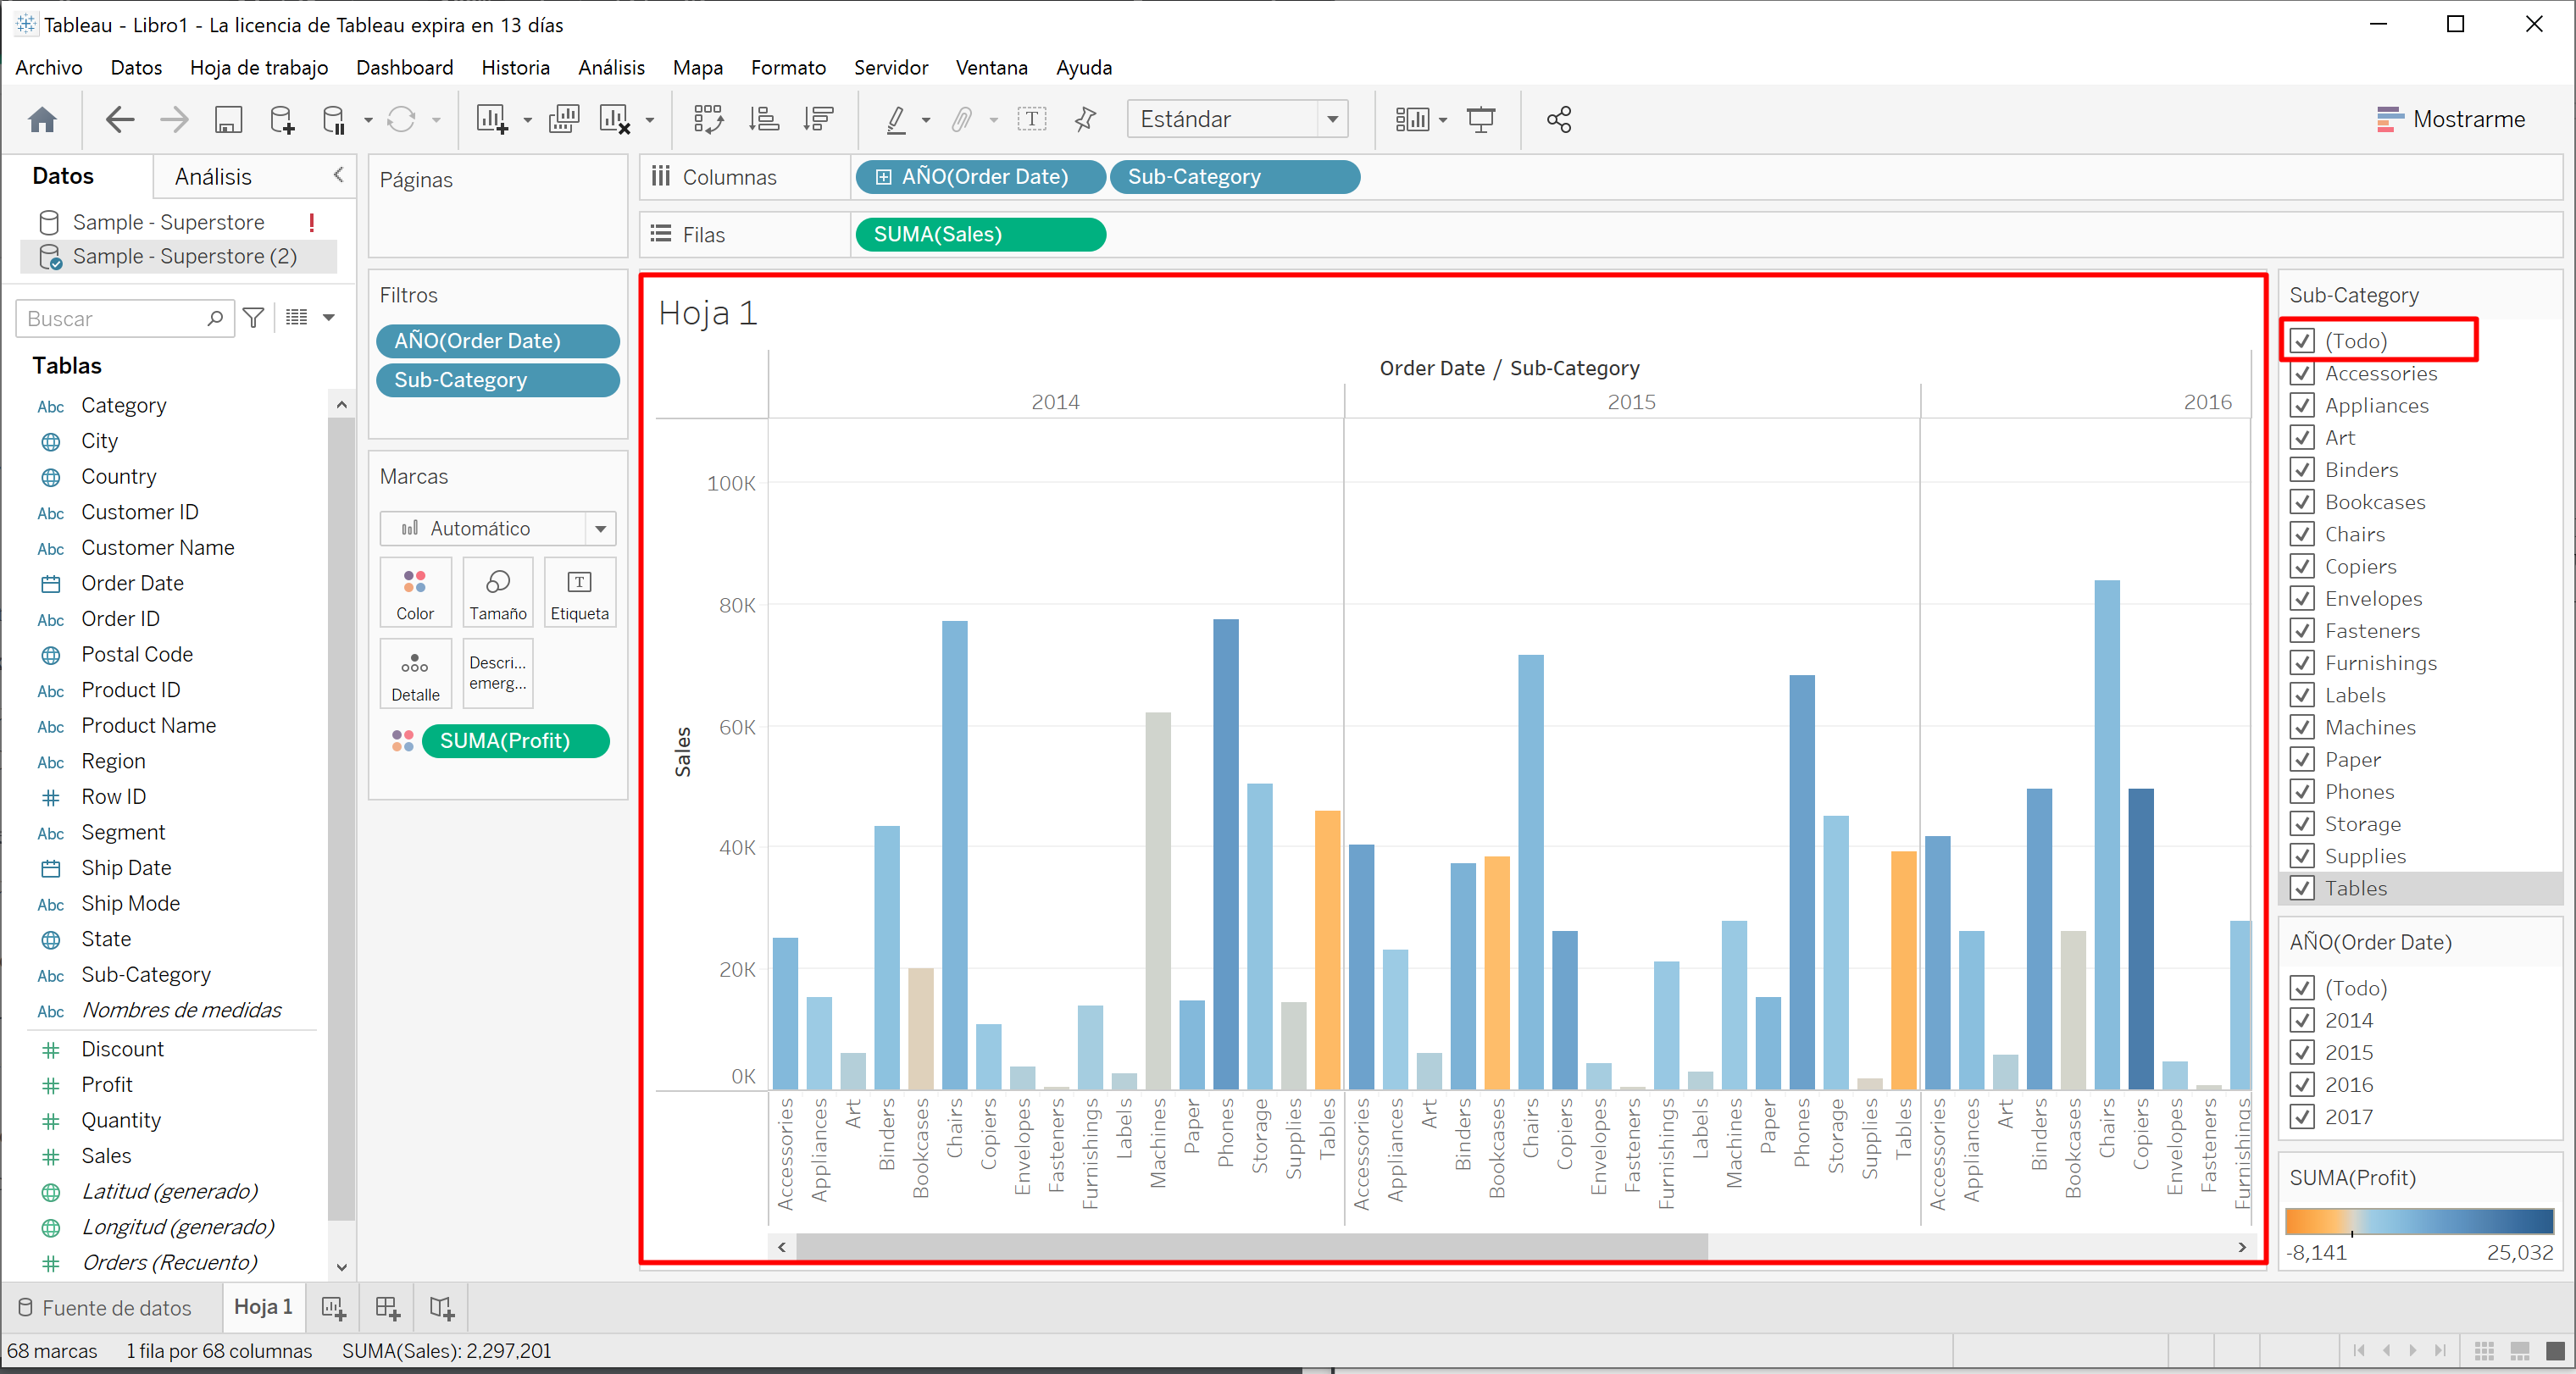
\includegraphics[width=16cm]{img/15.png}  
\end{center}
3. Desde Dimensiones, arrastre Region al Rows estante y colóquelo a la izquierda de la pestaña
Suma (Ventas). Observamos que las máquinas en el sur están reportando un beneficio negativo
mayor en general que en sus otras regiones.
\begin{center}
    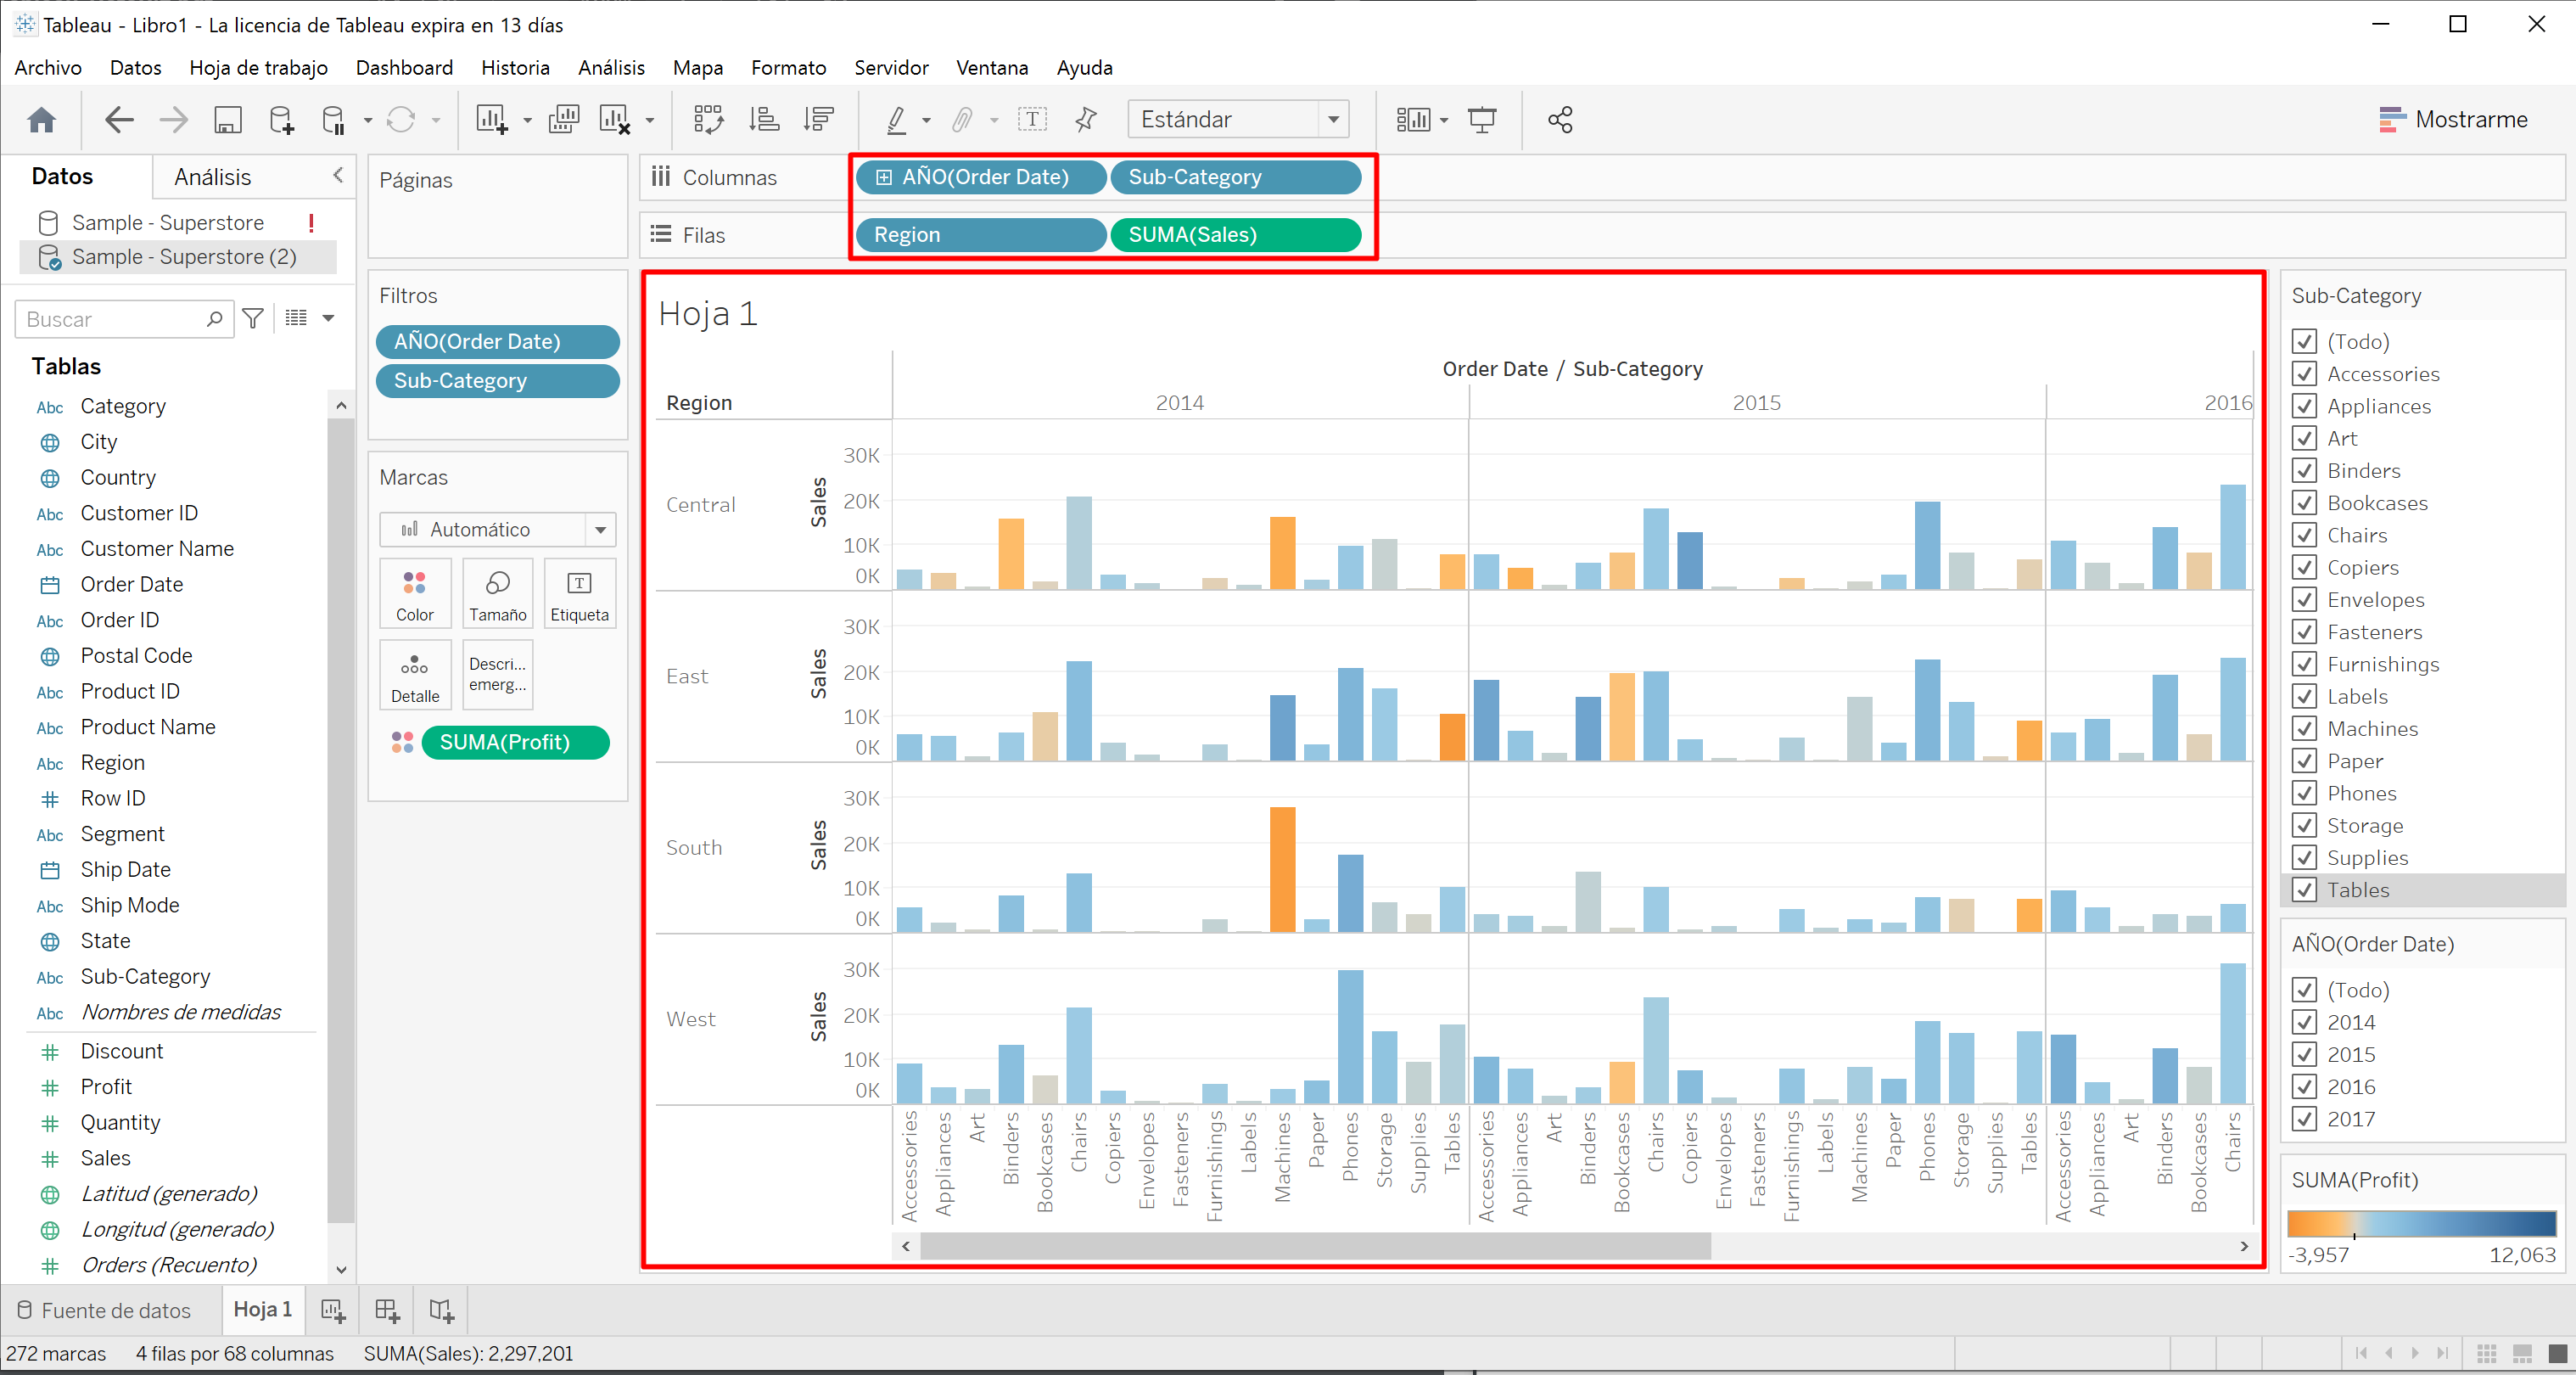
\includegraphics[width=16cm]{img/16.png}  
\end{center}
4. Démosle ahora un nombre a la hoja. En la parte inferior izquierda del espacio de trabajo, haga
doble clic Sheet 1y escriba Sales by Product and Region.
\begin{center}
    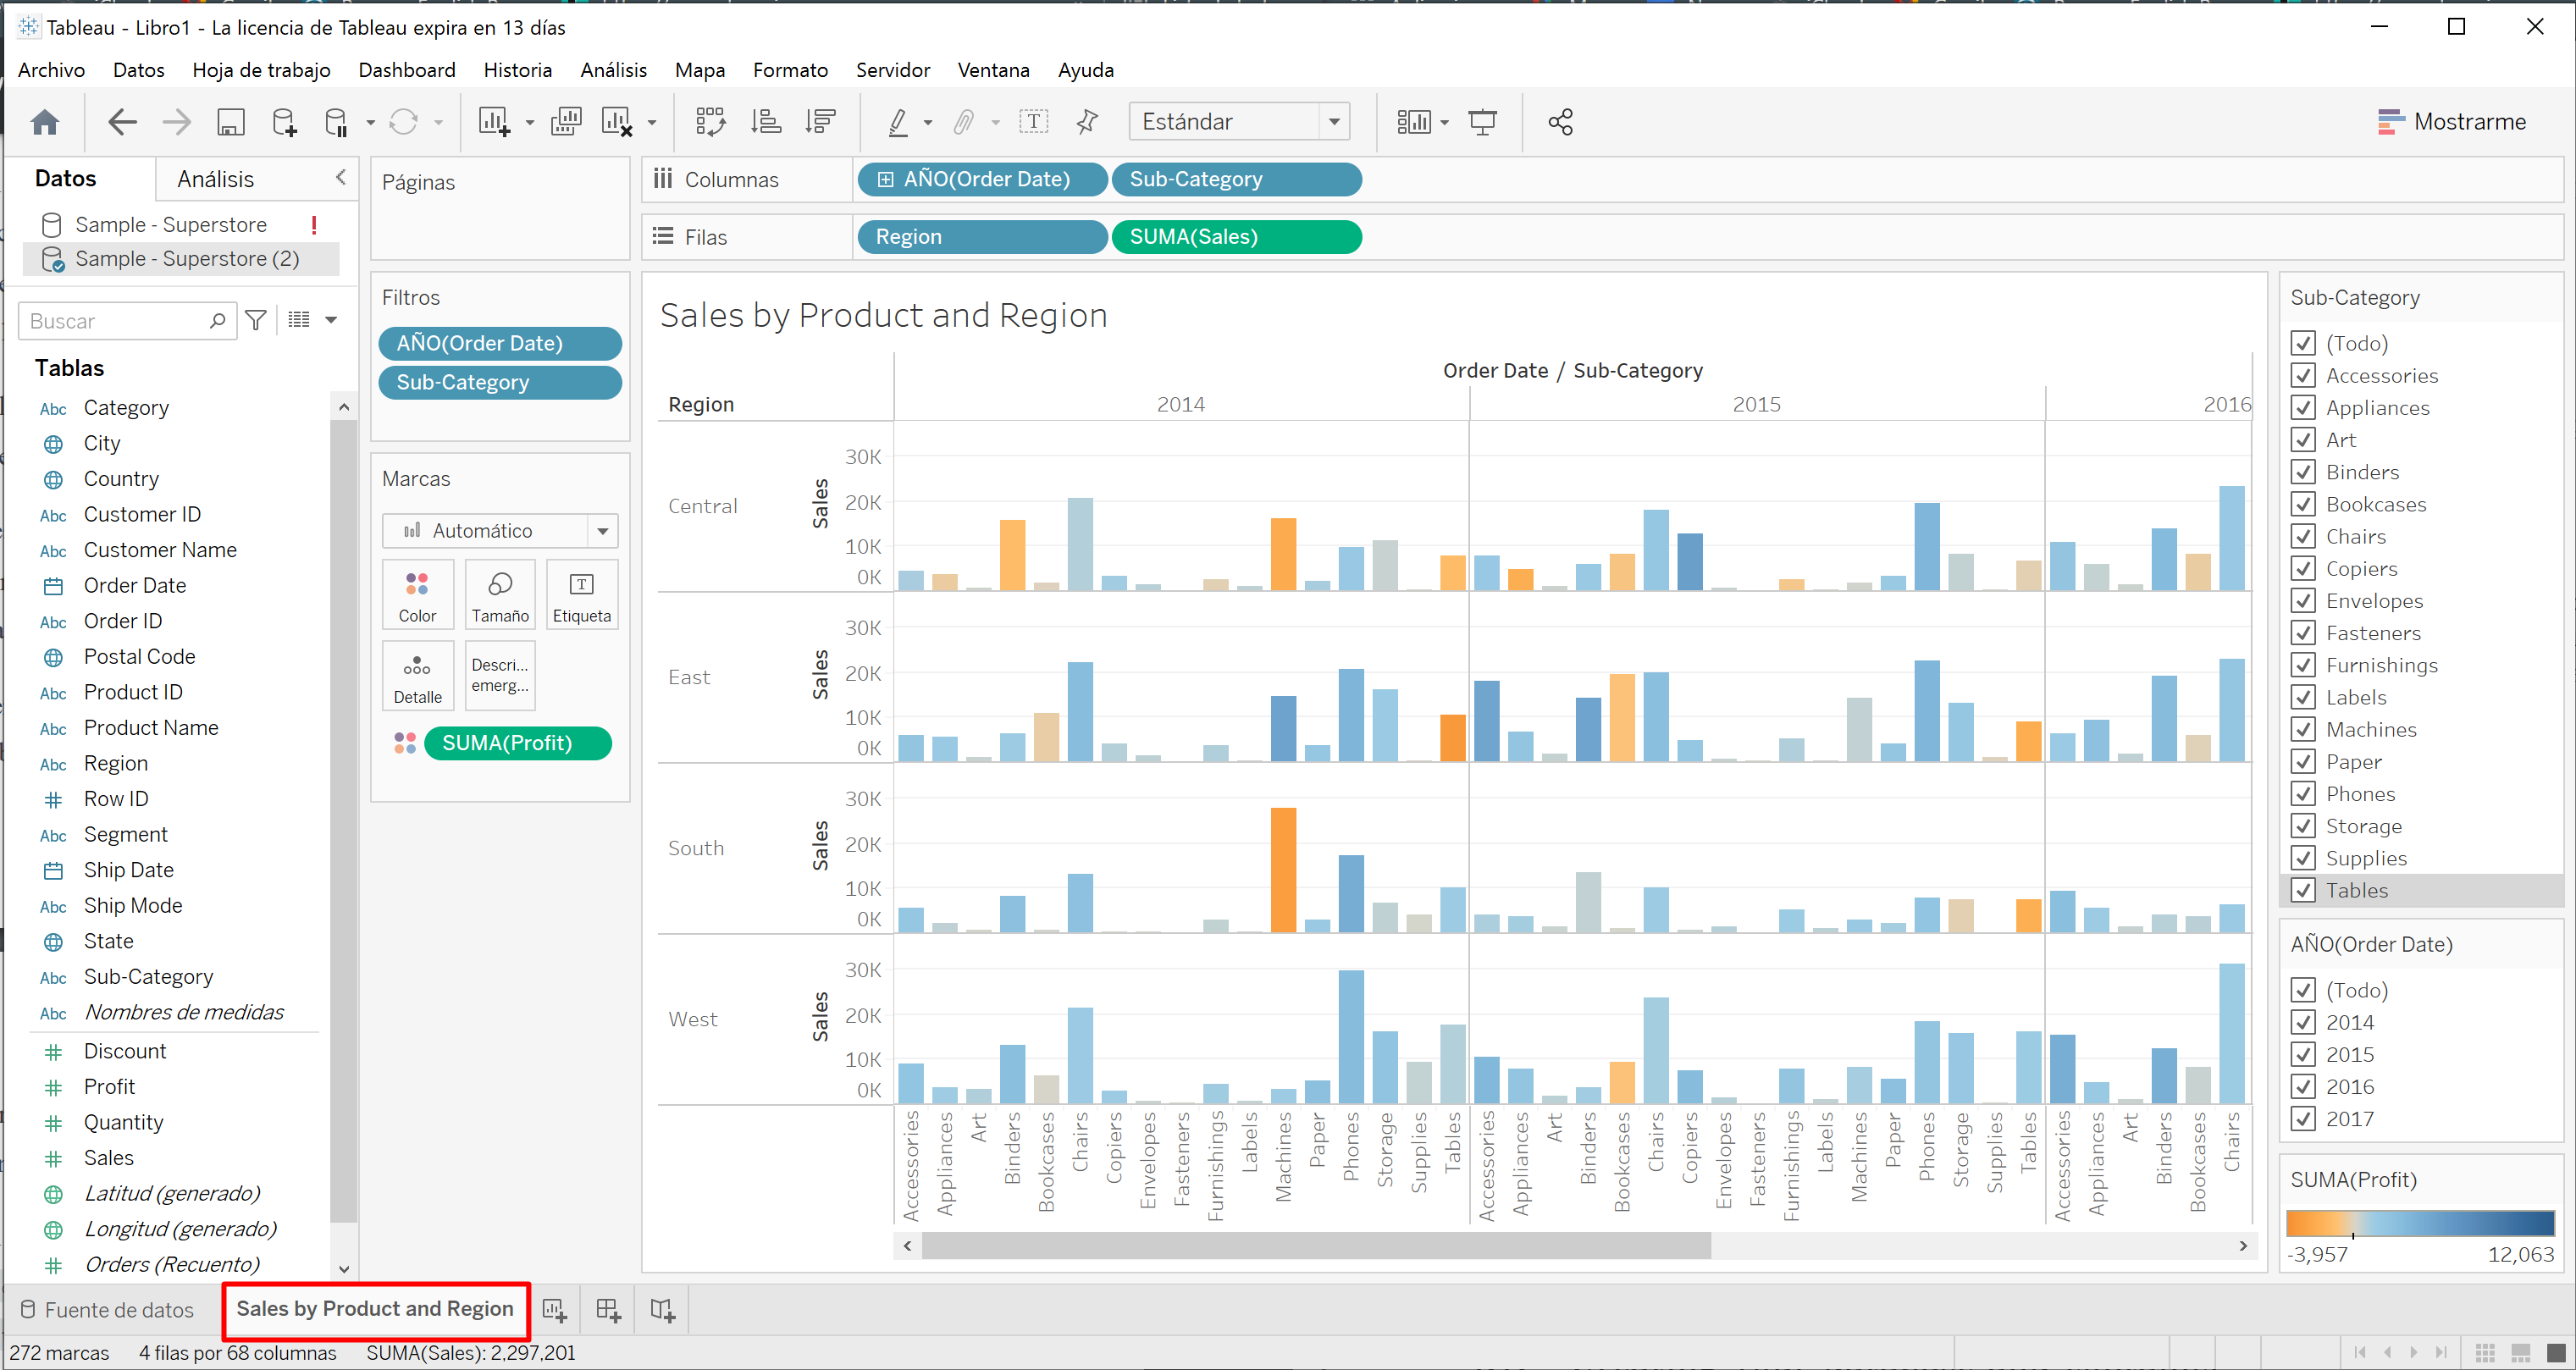
\includegraphics[width=16cm]{img/17.png}  
\end{center}
5. Para conservar la vista, Tableau nos permite duplicar nuestra hoja de trabajo para que podamos
\\\\6. En su libro de trabajo, haga clic con el botón derecho en la Sales by Product and
Regionhoja y seleccione Duplicatey cambie el nombre de la hoja duplicada a SalesSouth.
\begin{center}
    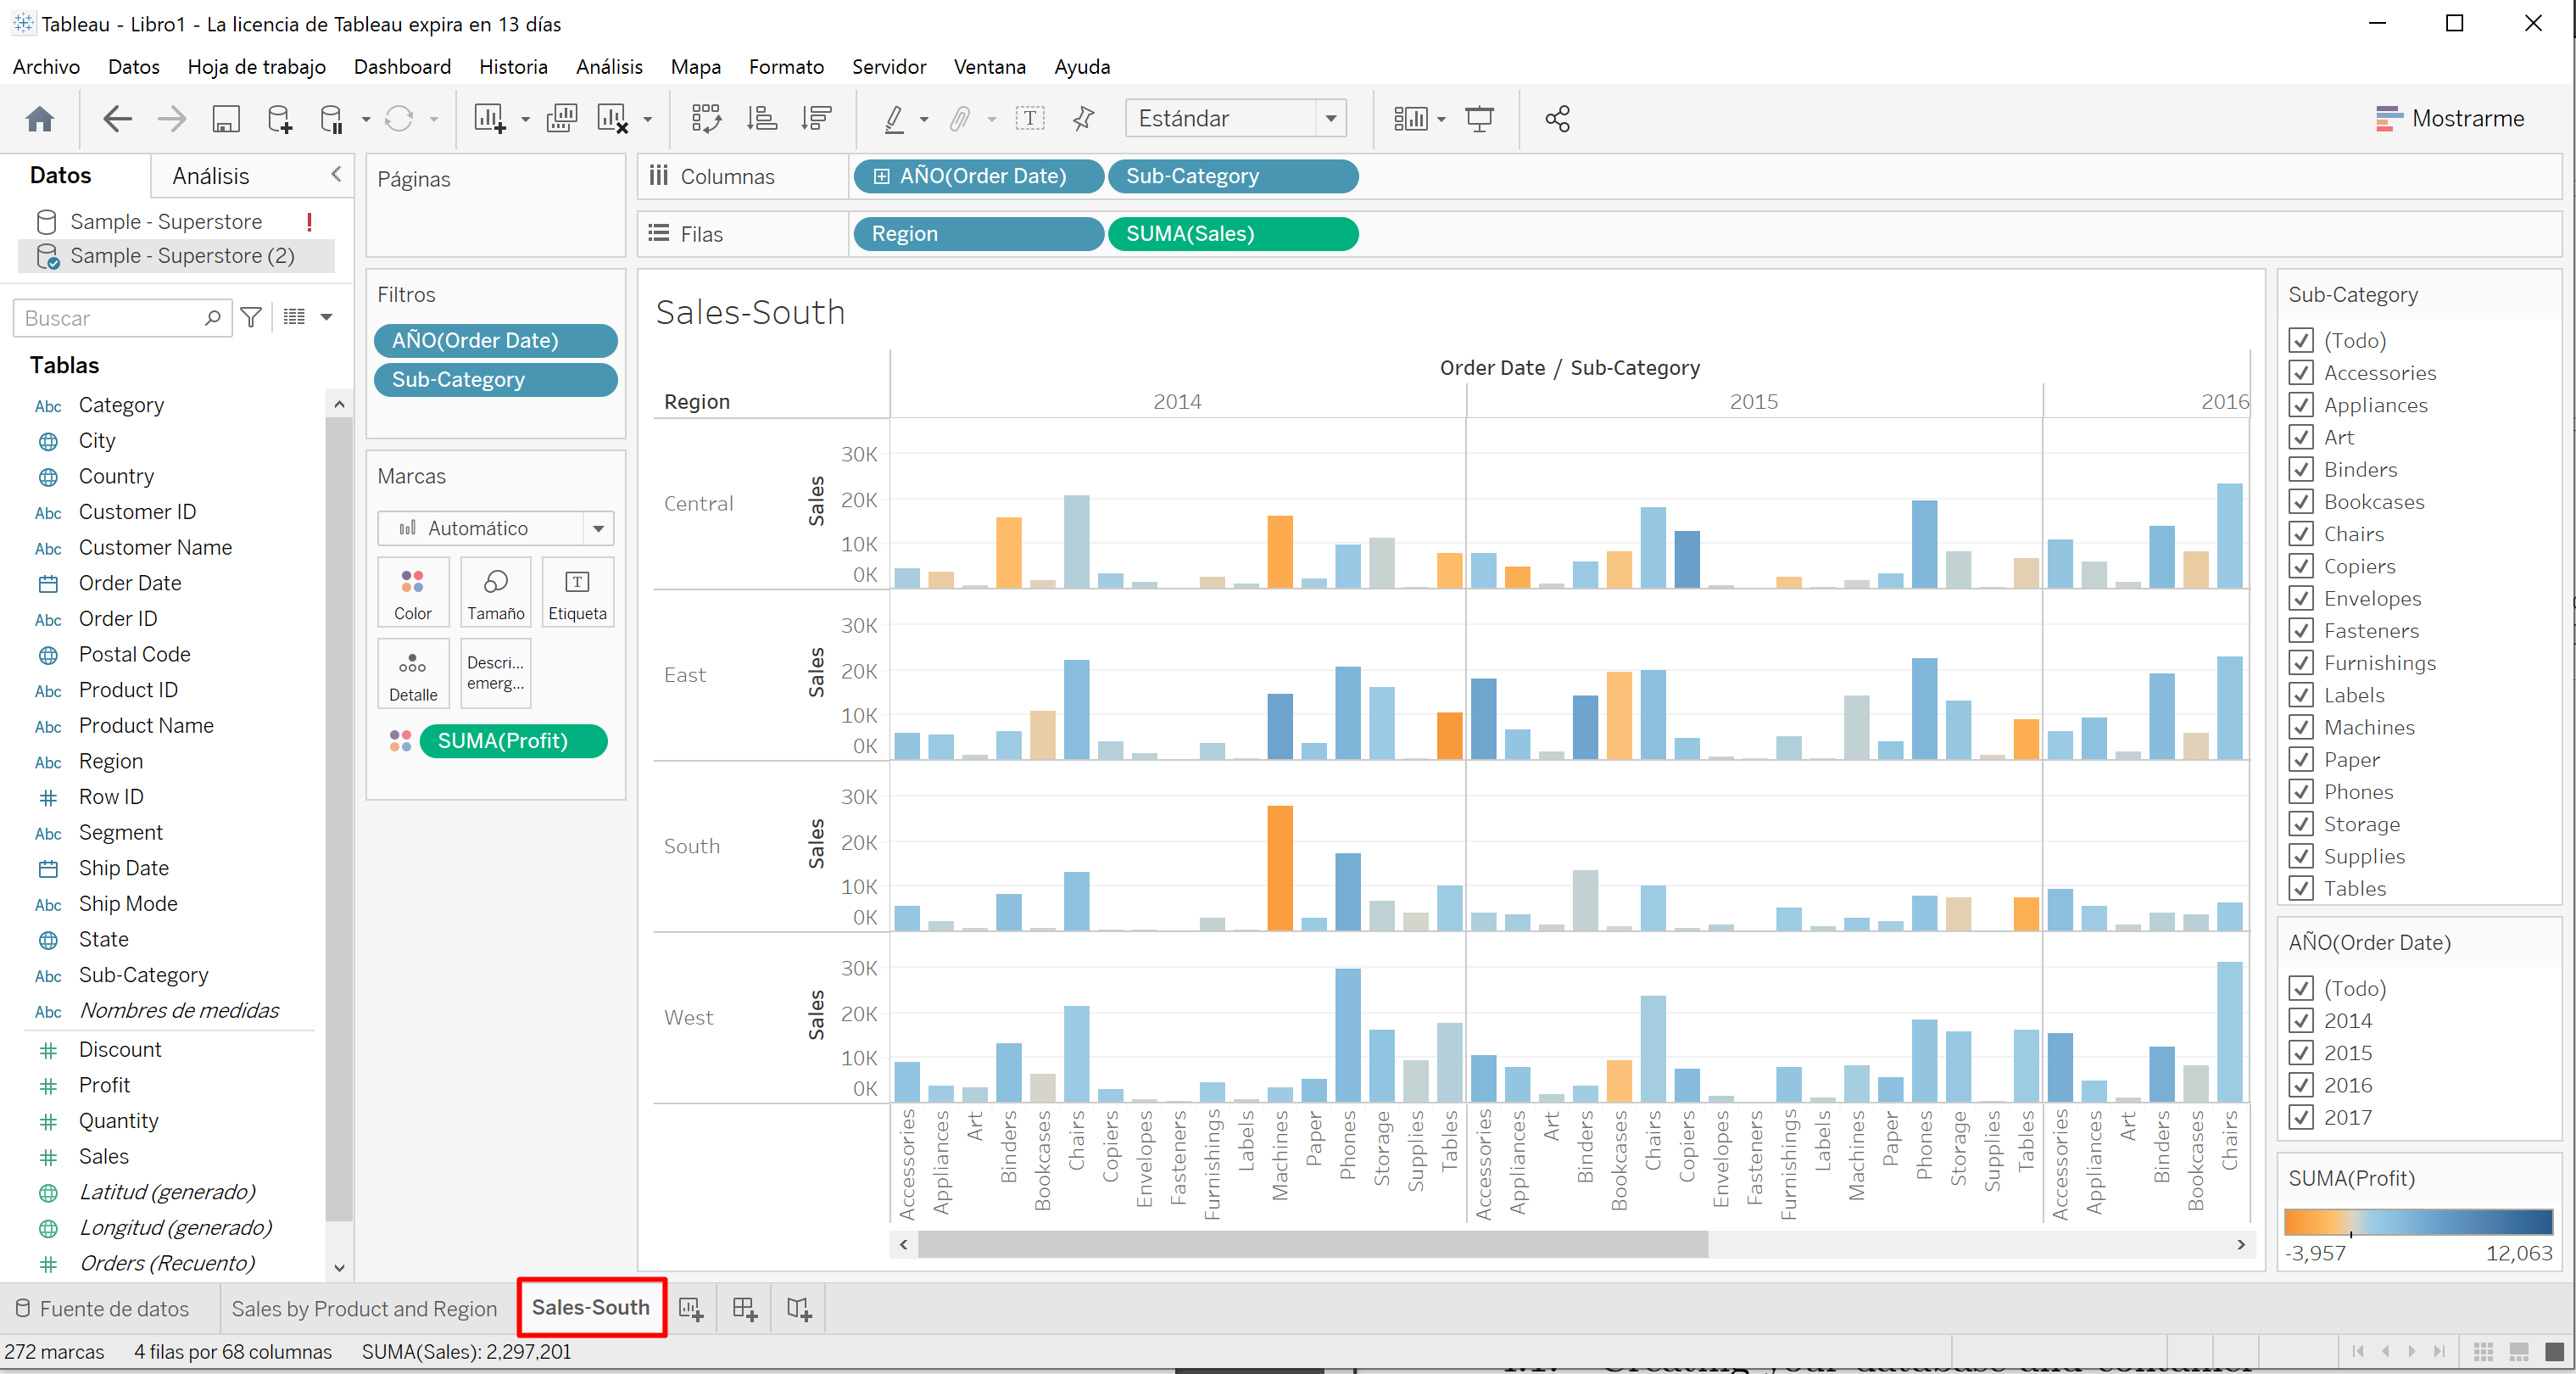
\includegraphics[width=16cm]{img/18.png}  
\end{center}
7. En la nueva hoja de trabajo, desde Dimensiones, arrastre Regional Filtersestante para
agregarlo como un filtro en la vista.
\begin{center}
    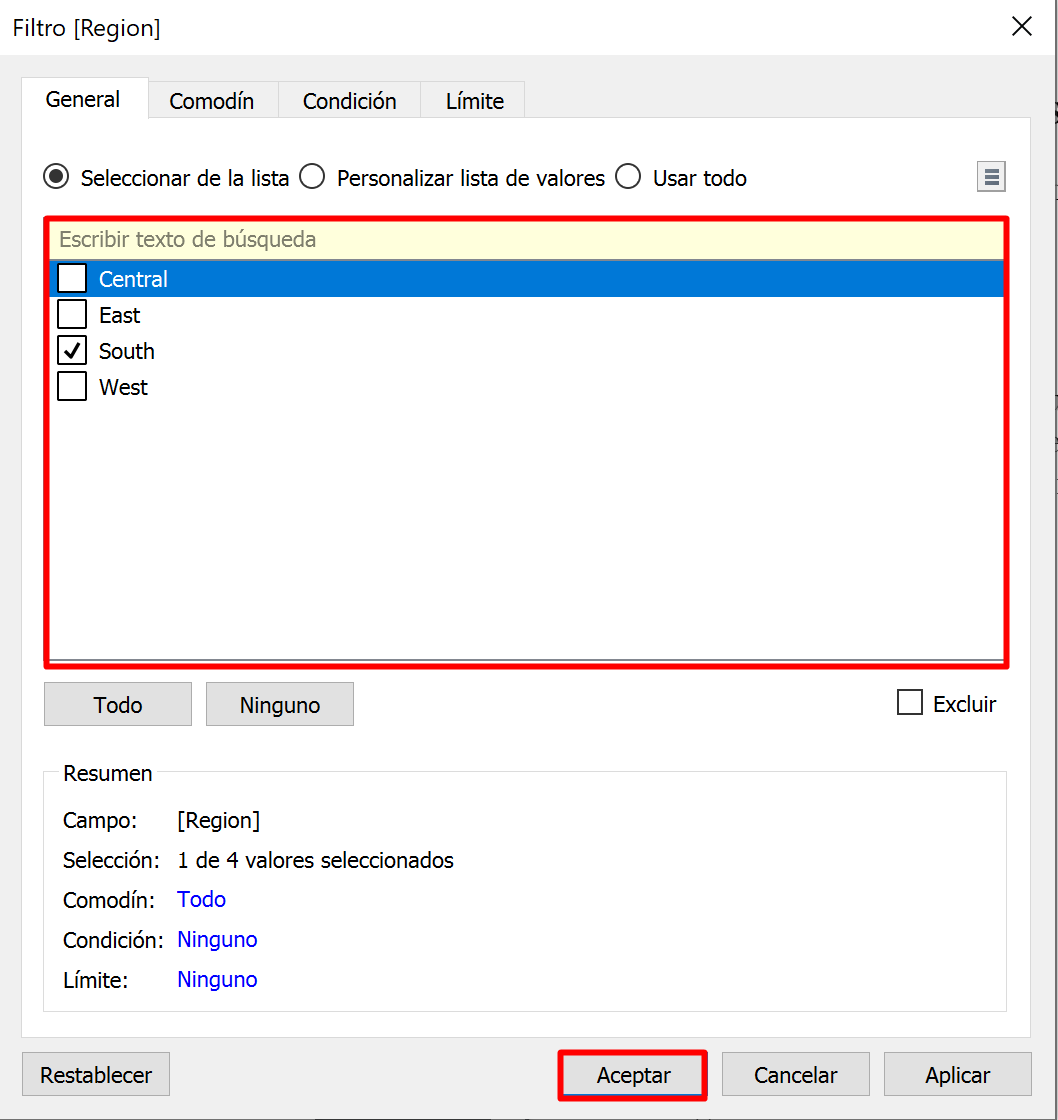
\includegraphics[width=10cm]{img/19.png}  
\end{center}
8. En el cuadro de diálogo Región de filtro, desactive todas las casillas de verificación excepto Sur
y luego haga clic en OK. Ahora podemos centrarnos en las ventas y las ganancias
en South. Descubrimos que las ventas de máquinas tuvieron un beneficio negativo en 2014 y
nuevamente en 2016. Investigaremos esto en la siguiente sección.
\begin{center}
    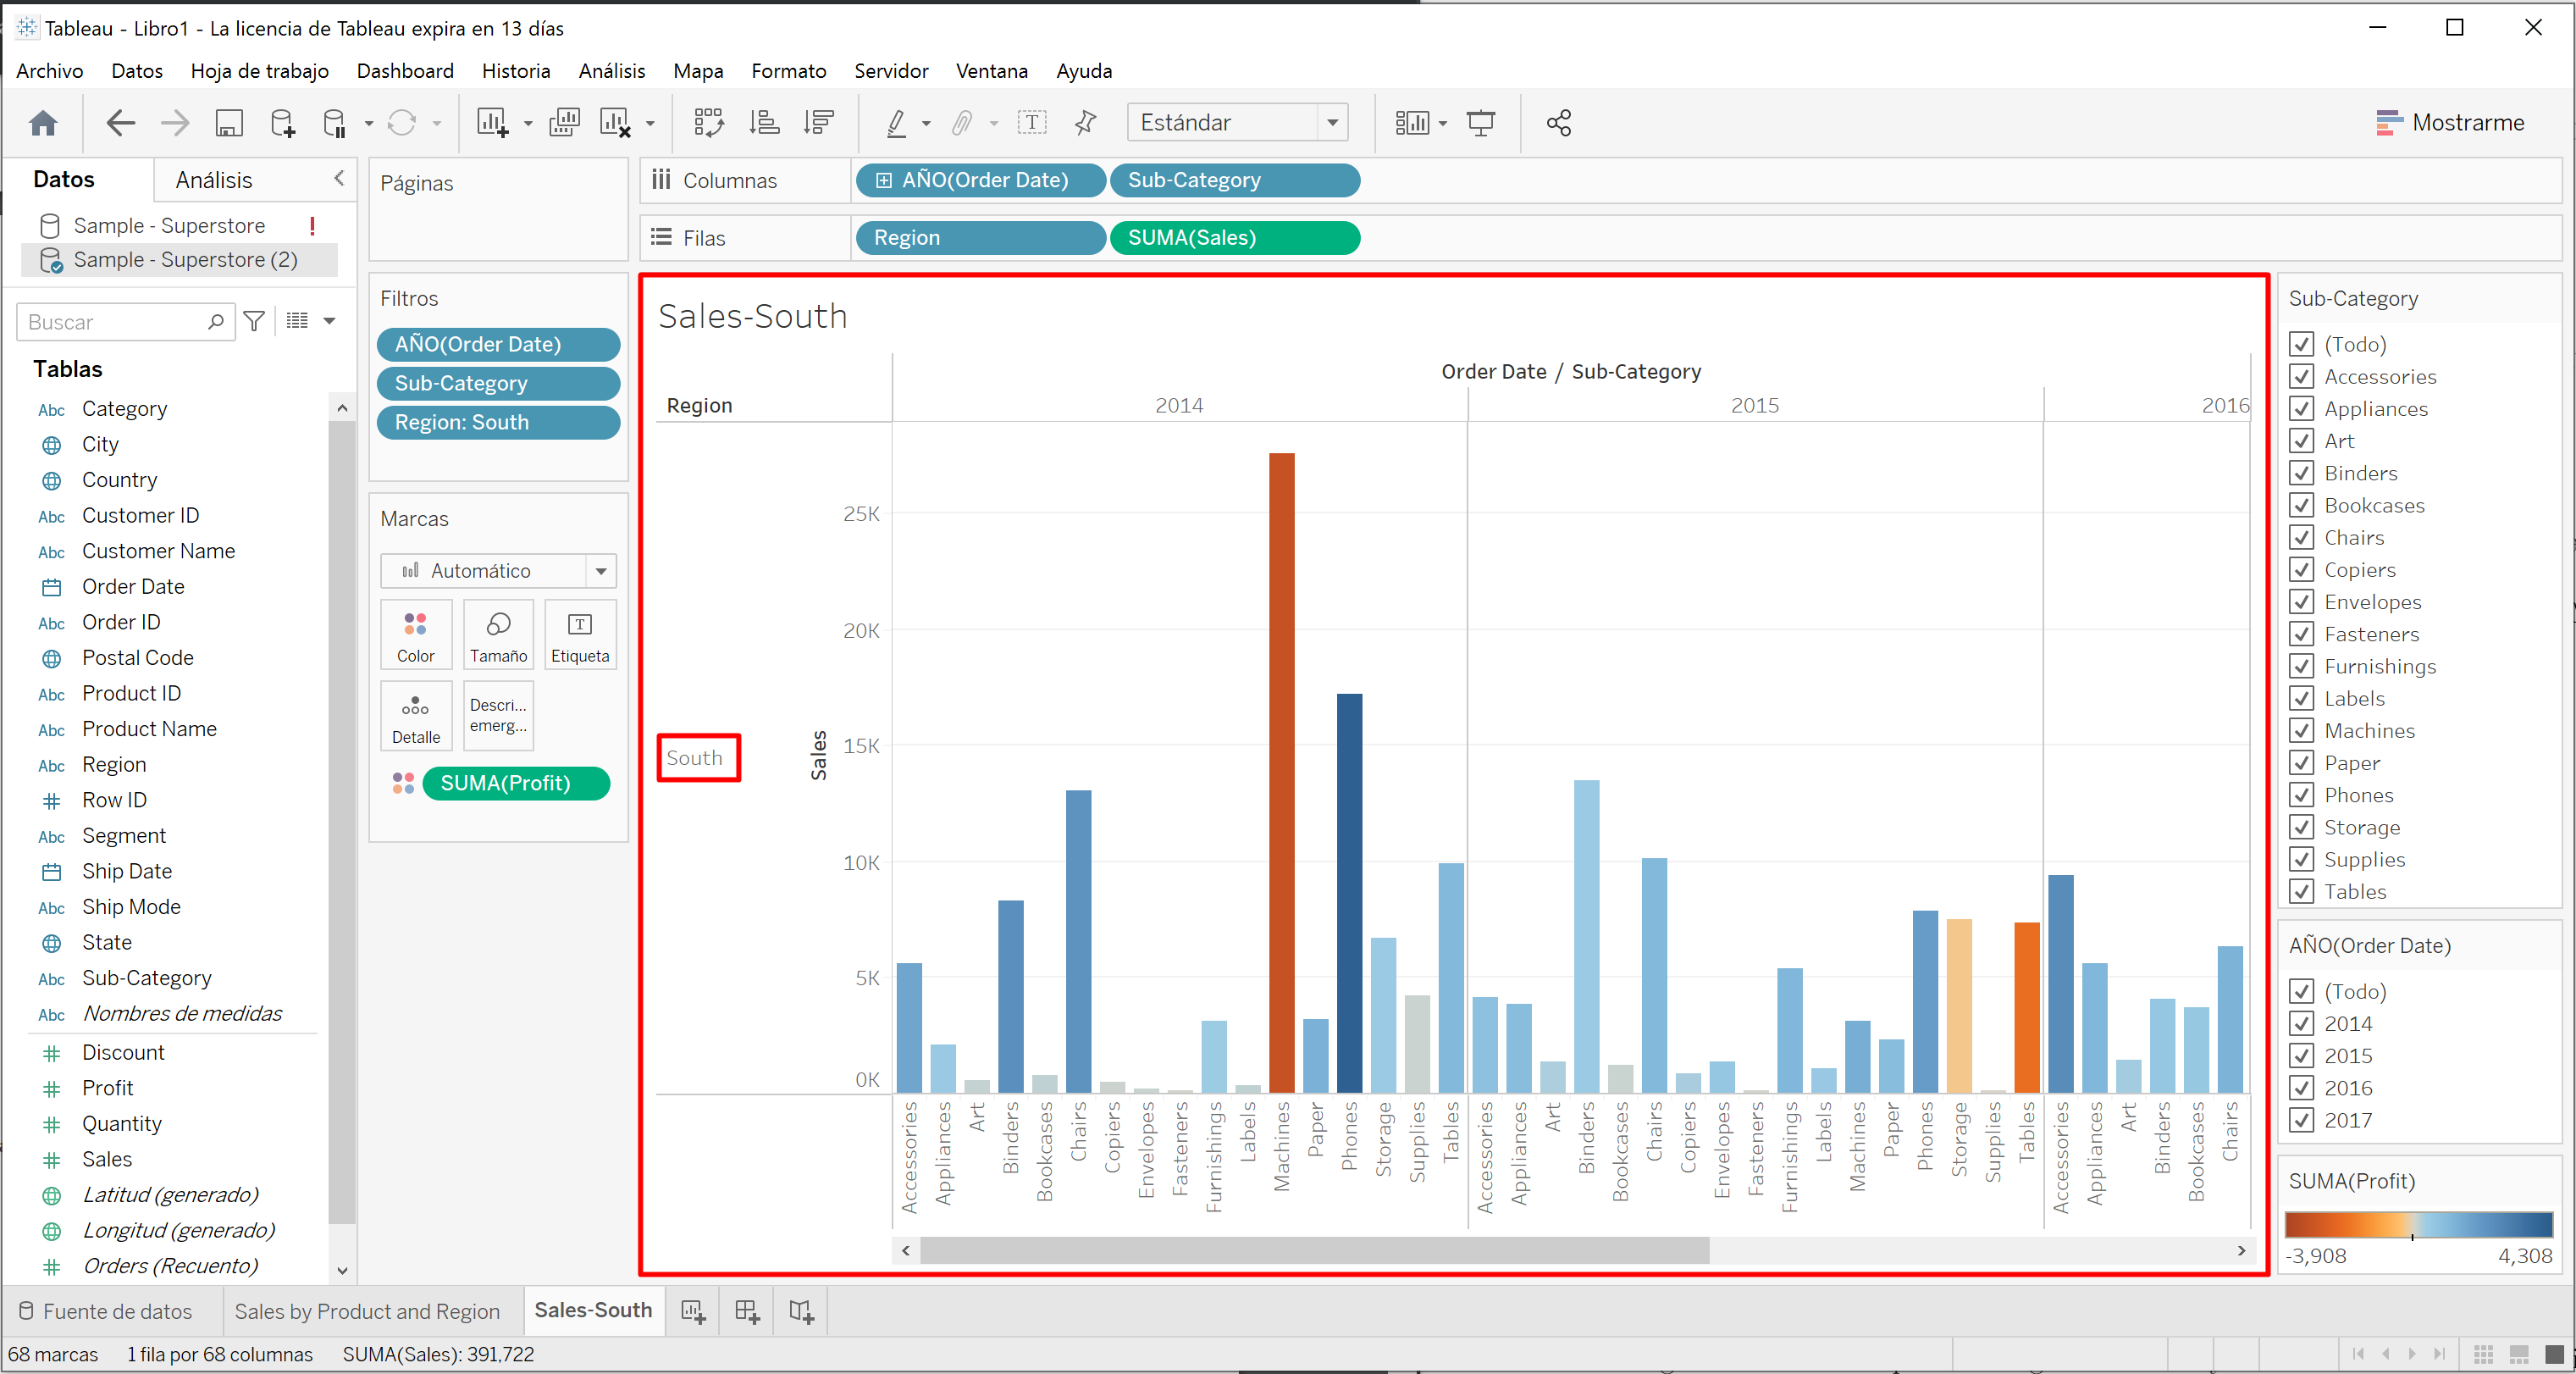
\includegraphics[width=16cm]{img/20.png}  
\end{center}
9. Por último, no olvide guardar los resultados seleccionando File > Save As. Nombremos
nuestro libro de trabajo como Regional Sales and Profits.

\section{Vista de mapa}
\subsection{Crear una vista de mapa}
Las vistas de mapa son beneficiosas cuando buscamos datos geográficos (el campo
Región). En el ejemplo actual, Tableau reconoce automáticamente que los campos
País, Estado, Ciudad y Código postal contienen información geográfica.
\\\\STEPS:
\\\\1. Crea una nueva hoja de trabajo.
\\\\2. Agregue State y Country en el panel Datos a Detail en la tarjeta Marcas. Obtenemos la
vista del mapa.
\begin{center}
    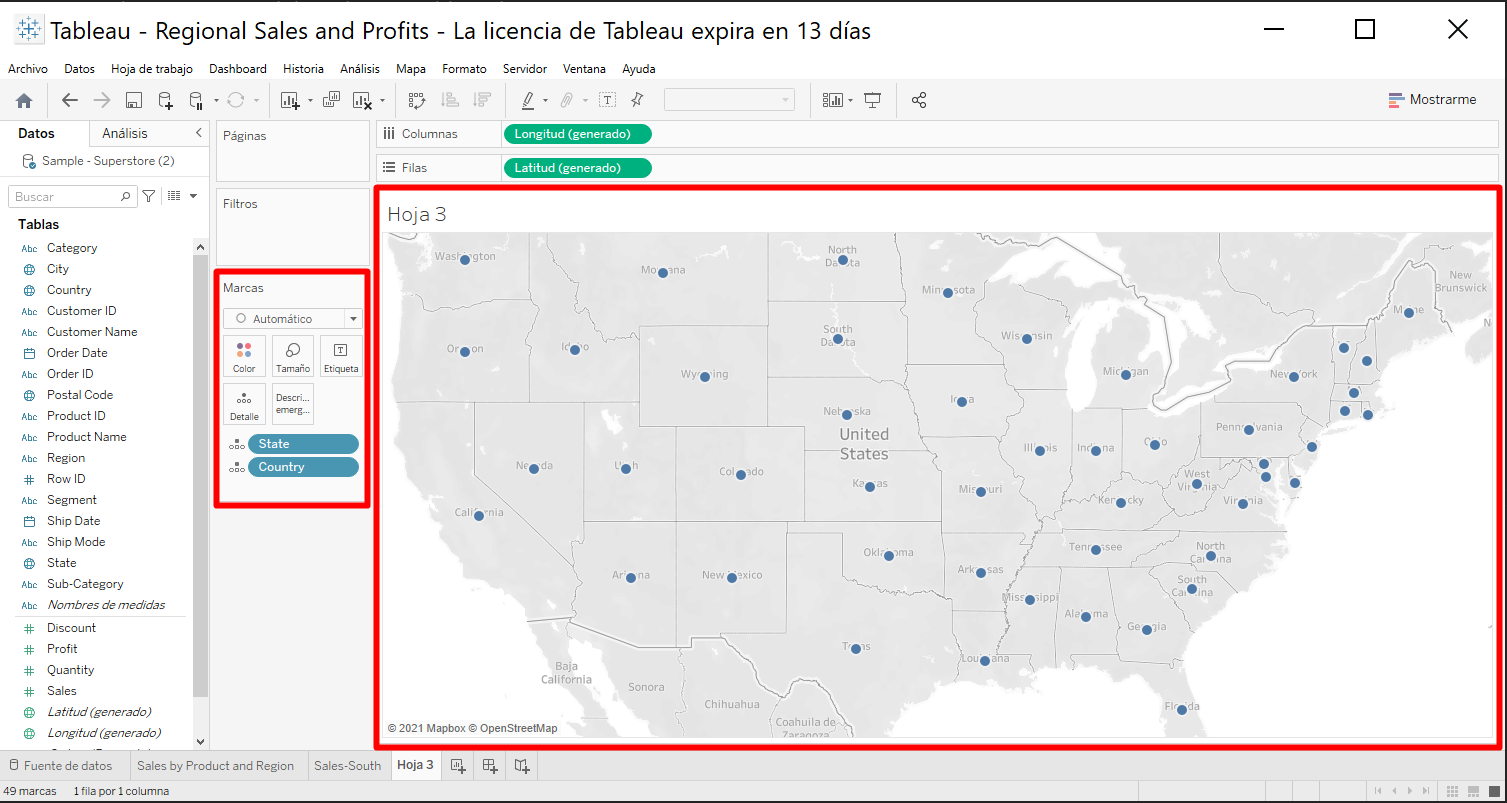
\includegraphics[width=16cm]{img/21.png}  
\end{center}
3. Arrastre Region a la Filters estantería y luego filtre hacia abajo South solo. La vista del
mapa ahora se acerca solo a la región Sur y una marca representa cada estado.
\begin{center}
    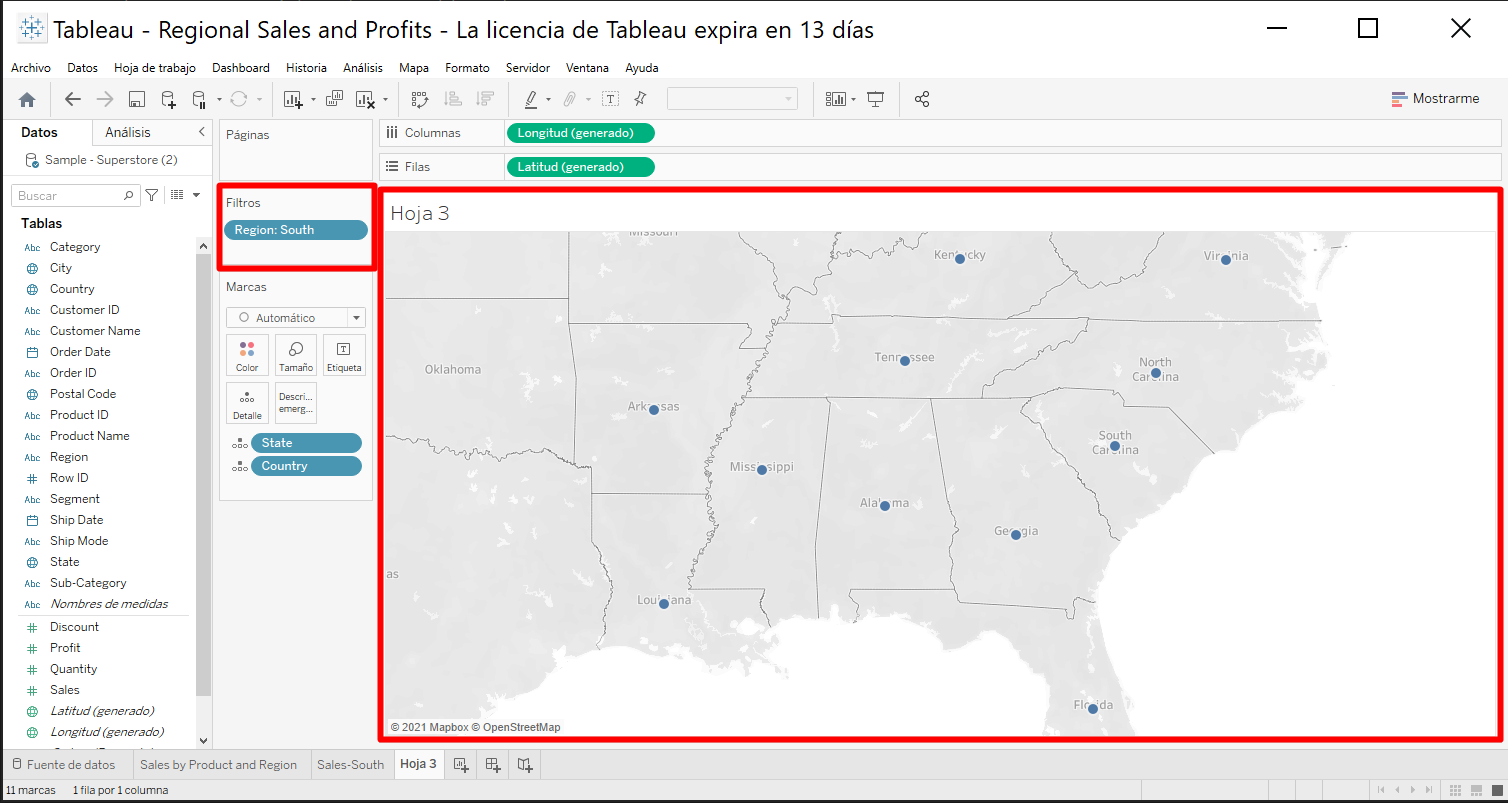
\includegraphics[width=16cm]{img/22.png}  
\end{center}
4. Arrastre la Sales medida a la Color pestaña de la tarjeta Marcas. Obtenemos un mapa relleno
con los colores que muestra el rango de ventas en cada estado.
\begin{center}
    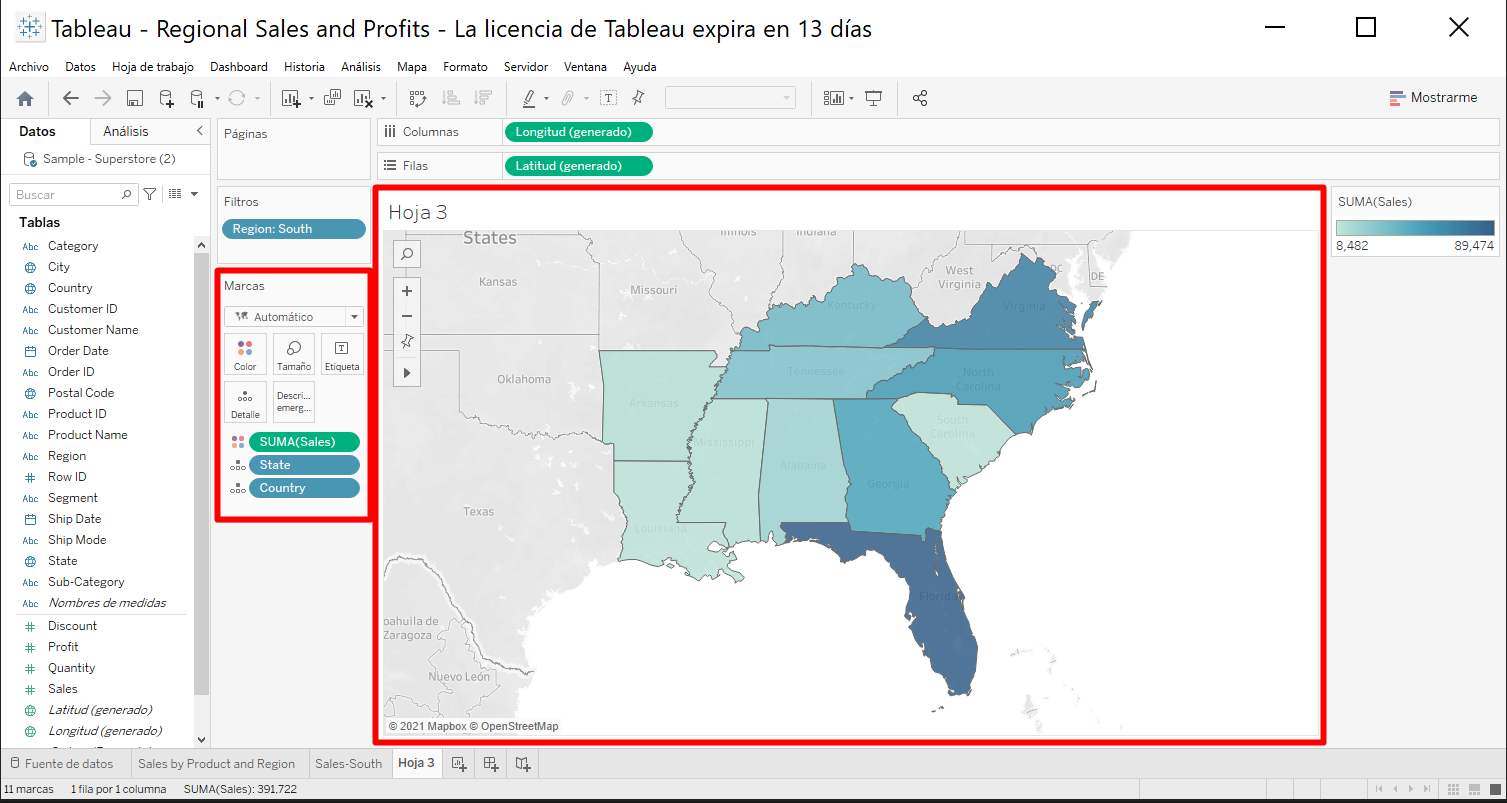
\includegraphics[width=16cm]{img/23.png}  
\end{center}
5. Podemos cambiar el esquema de color haciendo clic Color en la tarjeta Marcas y
seleccionando Edit Colors. Podemos experimentar con las paletas disponibles.
\begin{center}
    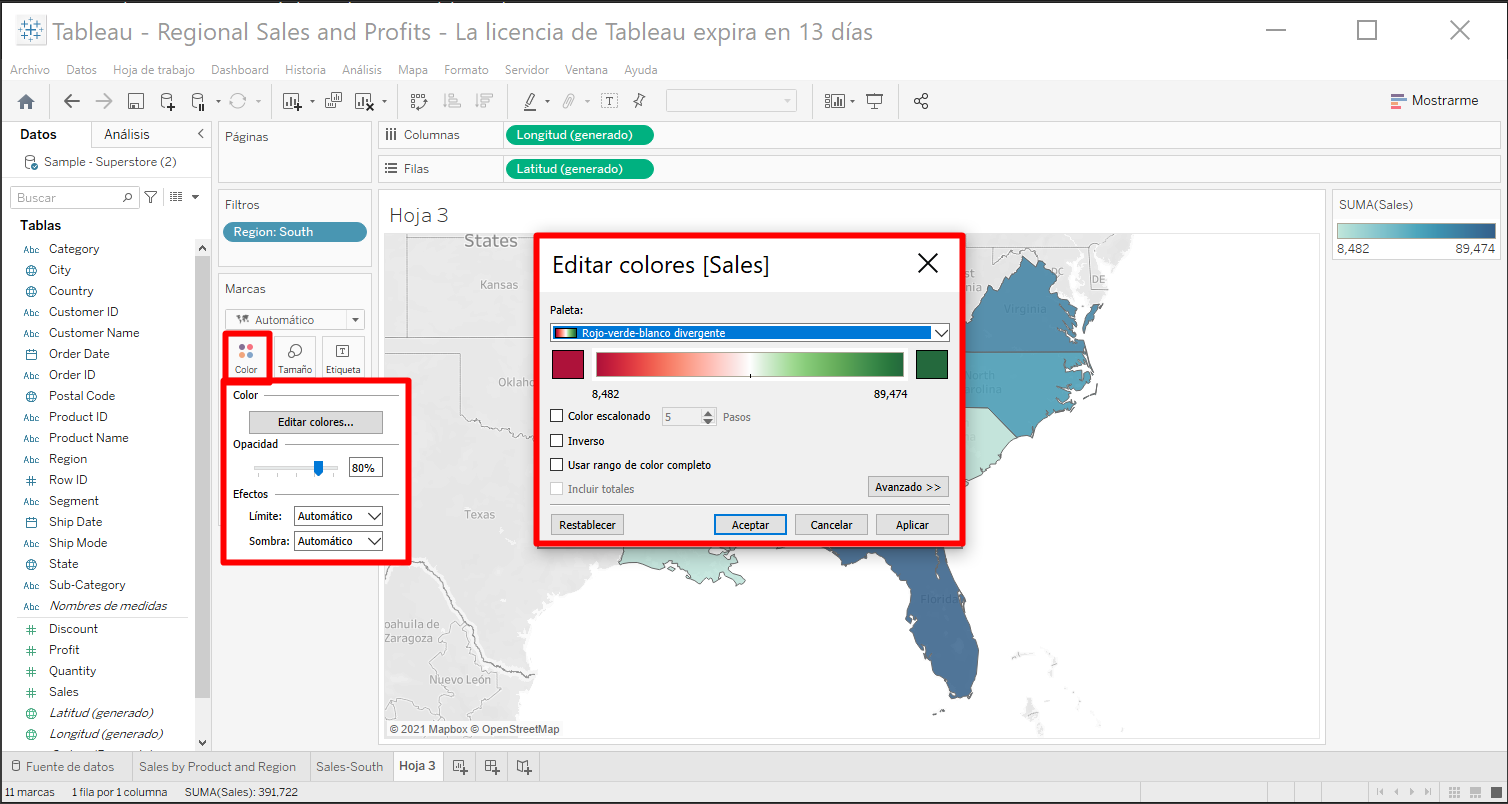
\includegraphics[width=16cm]{img/24.png}  
\end{center}
6. Observamos que Florida se está desempeñando mejor en ventas. Si pasamos el cursor sobre
Florida, muestra un total de 89,474 USD en ventas, en comparación con Carolina del Sur, por
ejemplo, que tiene solo 8,482 USD en ventas. Evaluemos el rendimiento a Profit estas
alturas, ya que las ganancias son un mejor indicador que las ventas por sí solas.
\begin{center}
    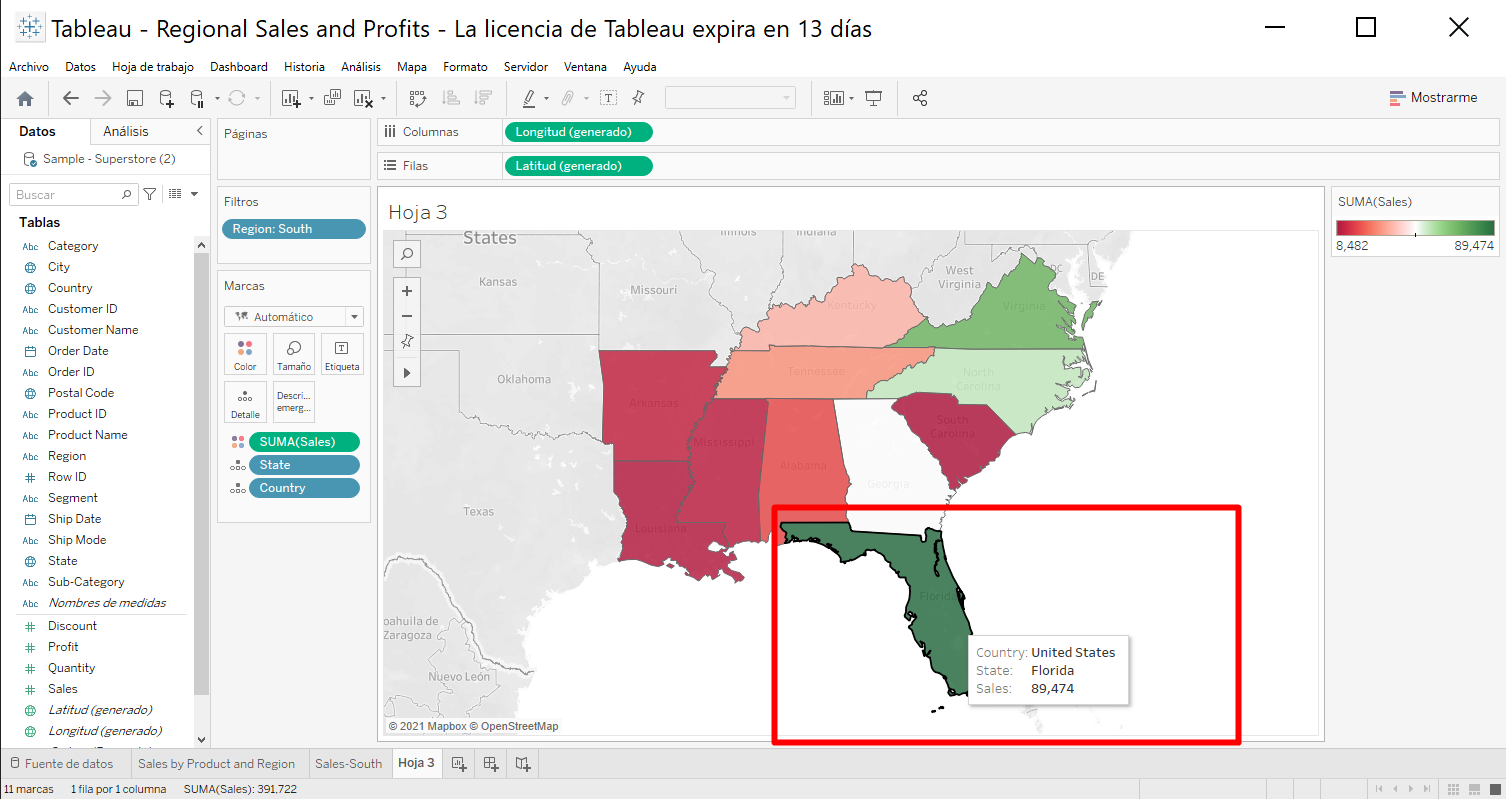
\includegraphics[width=16cm]{img/25.png}  
\end{center}
7. Arrastre Profit hacia Color en la tarjeta Marcas. Ahora vemos que Tennessee, Carolina del
Norte y Florida tienen ganancias negativas, aunque parecía que les estaba yendo bien en
Ventas. Cambiar el nombre de la hoja como Profit Map
\begin{center}
    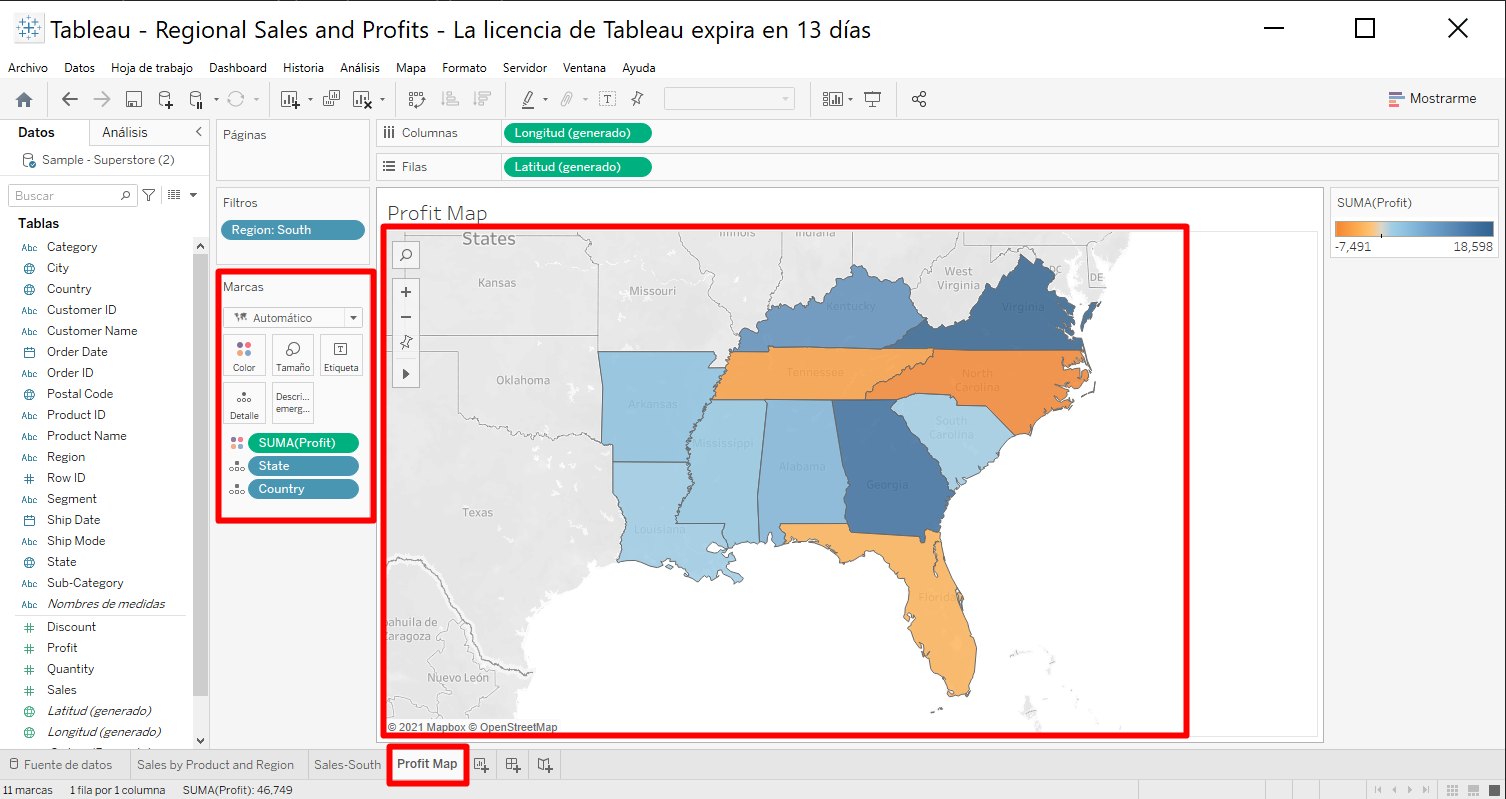
\includegraphics[width=16cm]{img/26.png}  
\end{center}

\subsection{Entrar en los detalles}
Los mapas nos permiten visualizar los datos de manera amplia. En el último paso,
descubrimos que descubrimos que Tennessee, Carolina del Norte y Florida tienen una
ganancia negativa. En esta sección dibujemos un gráfico de barras para explorar la
razón de la ganancia negativa
\\\\STEPS:
\\\\1. Duplique la hoja de trabajo Mapa de beneficios y asígnele el nombre Gráfico de barras de
beneficios negativos
\begin{center}
    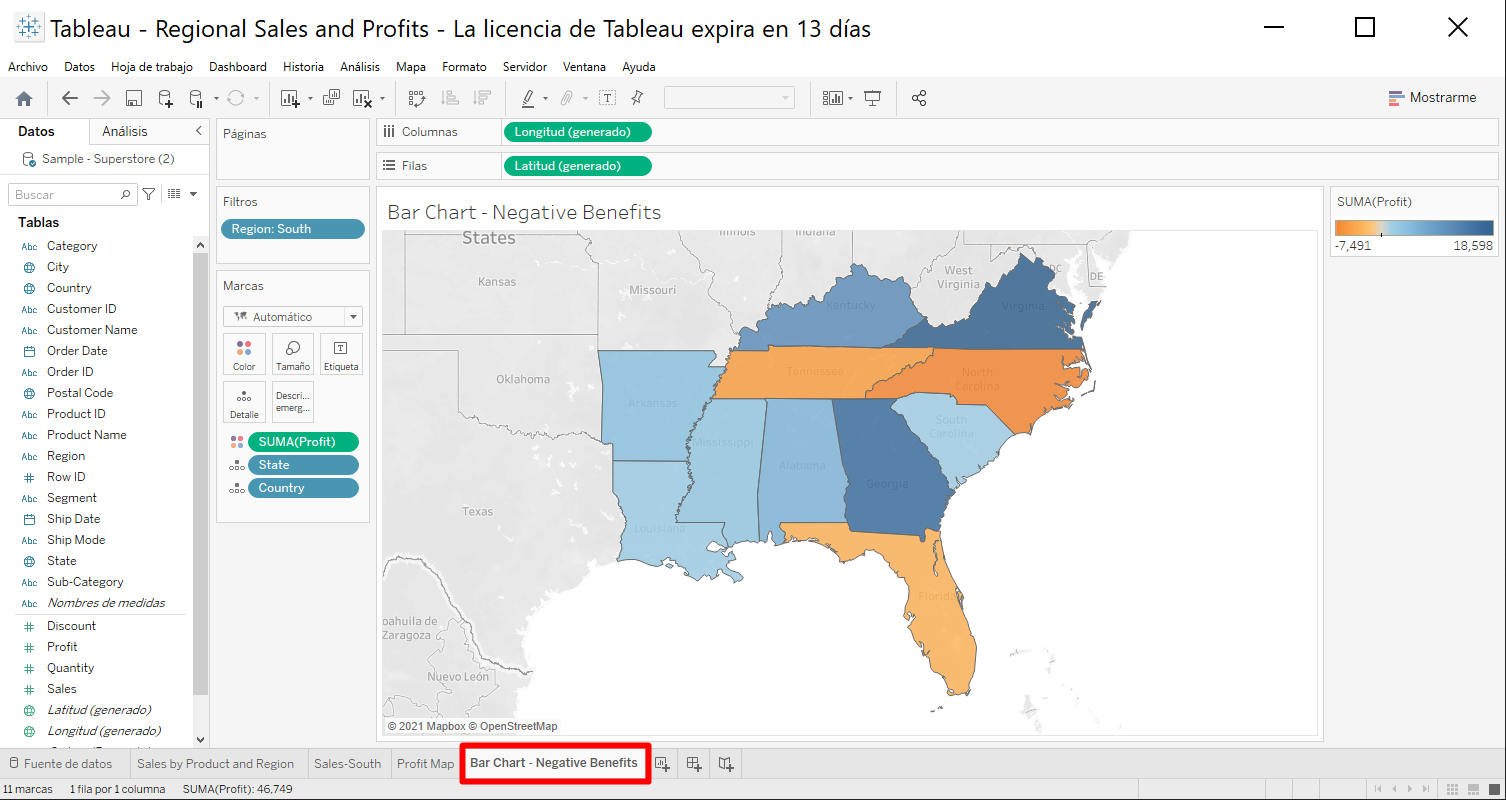
\includegraphics[width=16cm]{img/27.png}  
\end{center}
2. Haga clic Show Me en la hoja de trabajo Gráfico de barras de ganancias negativas . Show
Me presenta el número de formas en que se puede trazar un gráfico entre los elementos 
mencionados en la hoja de trabajo. De Show Me seleccionar la opción de la barra horizontal y
los cambios a vista horizontal de las barras verticales de forma instantánea.
\begin{center}
    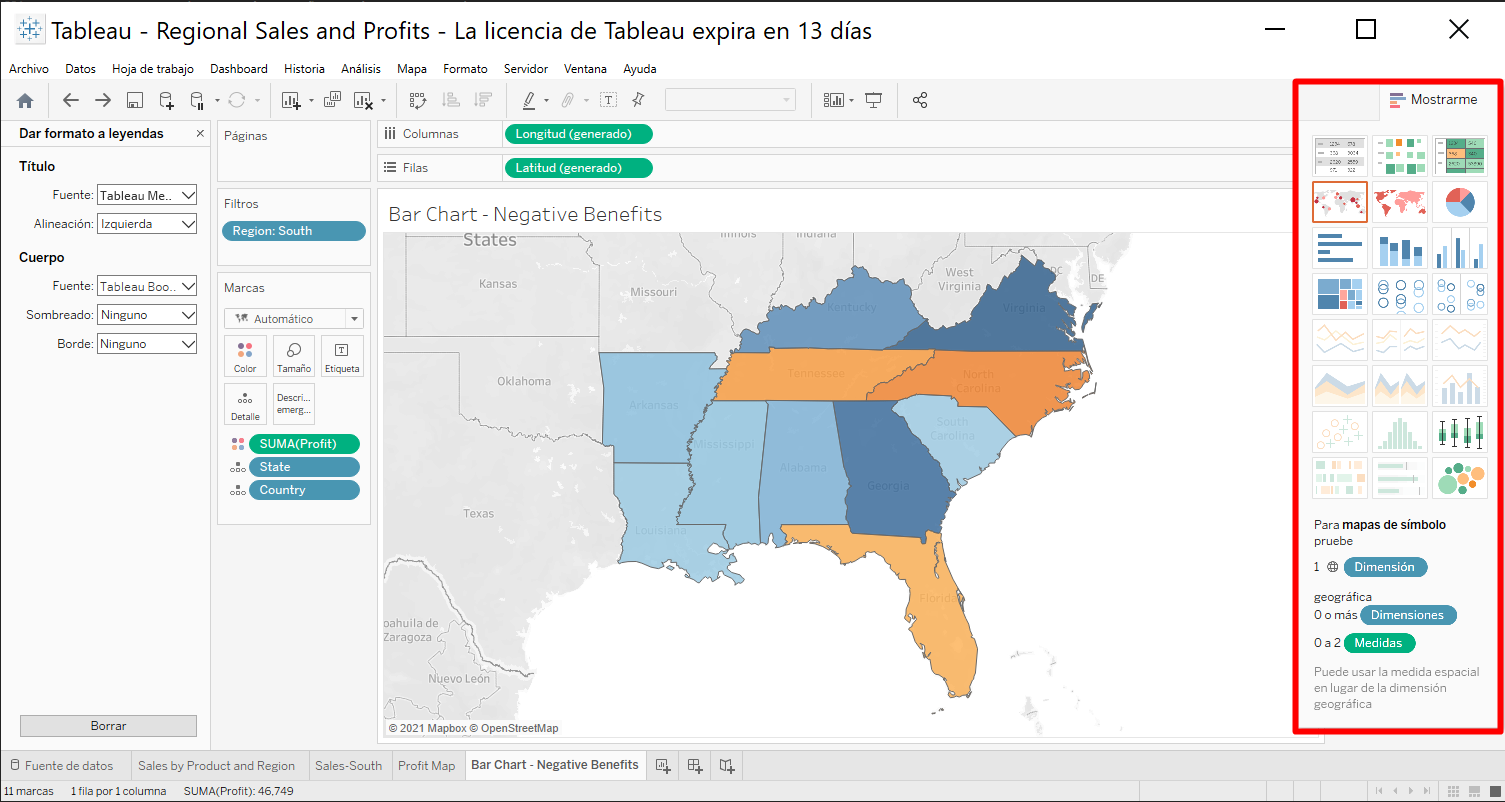
\includegraphics[width=16cm]{img/28.png}  
\end{center}
3. Podemos seleccionar más de una barra a la vez simplemente haciendo clic y arrastrando el
cursor sobre ellas. Queremos centrarnos únicamente en los tres estados, es decir, Tennessee,
Carolina del Norte y Florida. Por lo tanto, solo seleccionaremos las barras correspondientes.
\begin{center}
    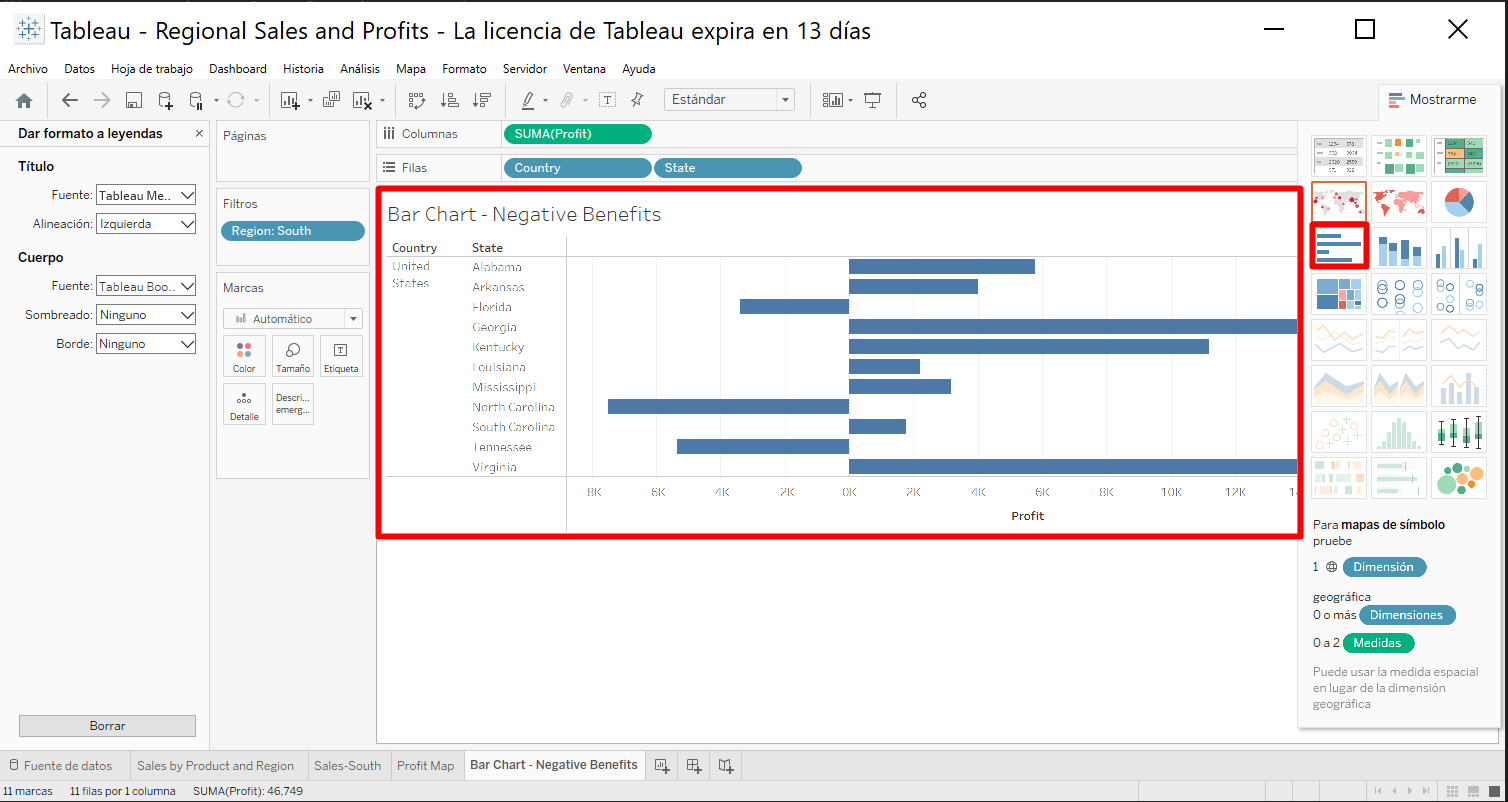
\includegraphics[width=16cm]{img/29.png}  
\end{center}

\subsection{Creación de jerarquías}
jerarquías son útiles cuando queremos agrupar campos similares para poder profundizar
rápidamente entre los niveles de la visualización.
\\\\1. En el panel Datos, arrastre un campo y suéltelo directamente encima de otro campo o haga clic
con el botón derecho en el campo y seleccione
\begin{center}
    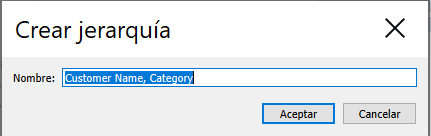
\includegraphics[width=8cm]{img/30.png}  
\end{center}
2. Arrastre cualquier campo adicional a la jerarquía. Los campos también se pueden reordenar en
la jerarquía simplemente arrastrándolos a una nueva posición. En la visualización
actual. Crearemos las siguientes jerarquías: Ubicación, Pedido y Producto.
\begin{center}
    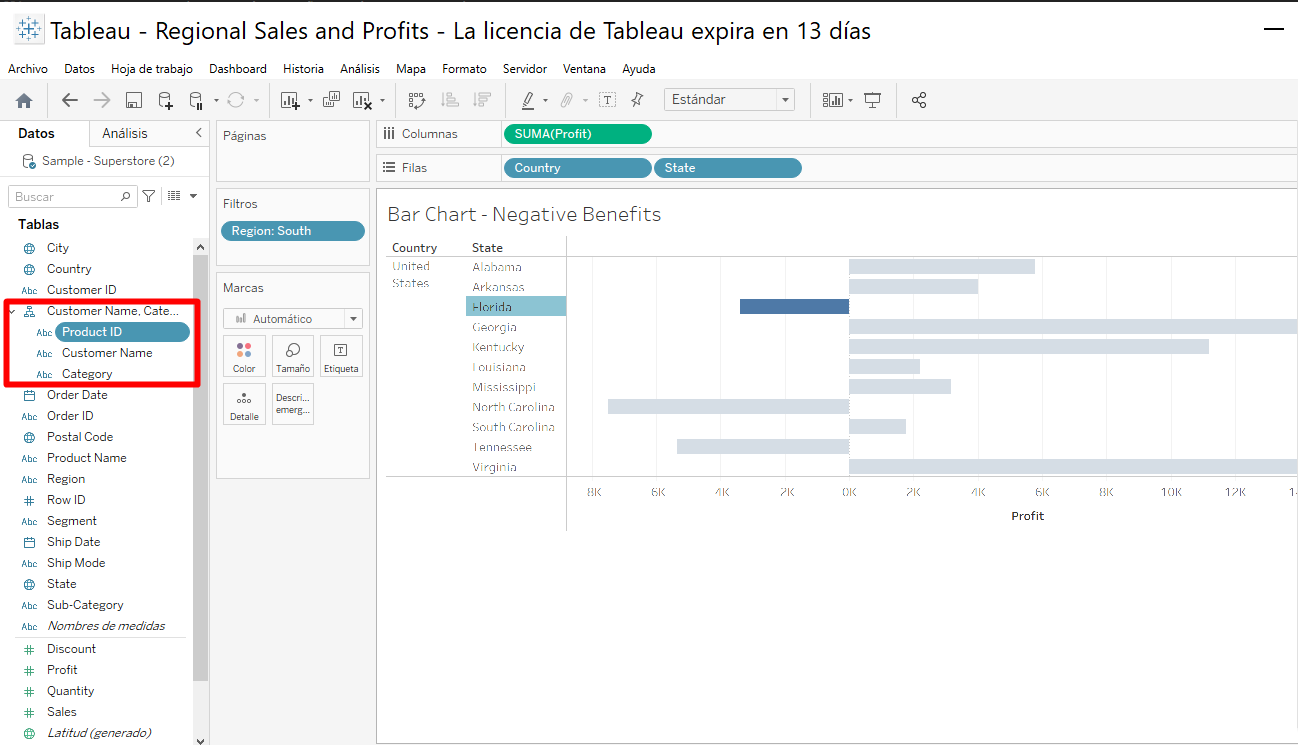
\includegraphics[width=16cm]{img/31.png}  
\end{center}
3. En el estante de filas, haga clic en el icono con forma de más en el State campo para desglosar
el City nivel.
\begin{center}
    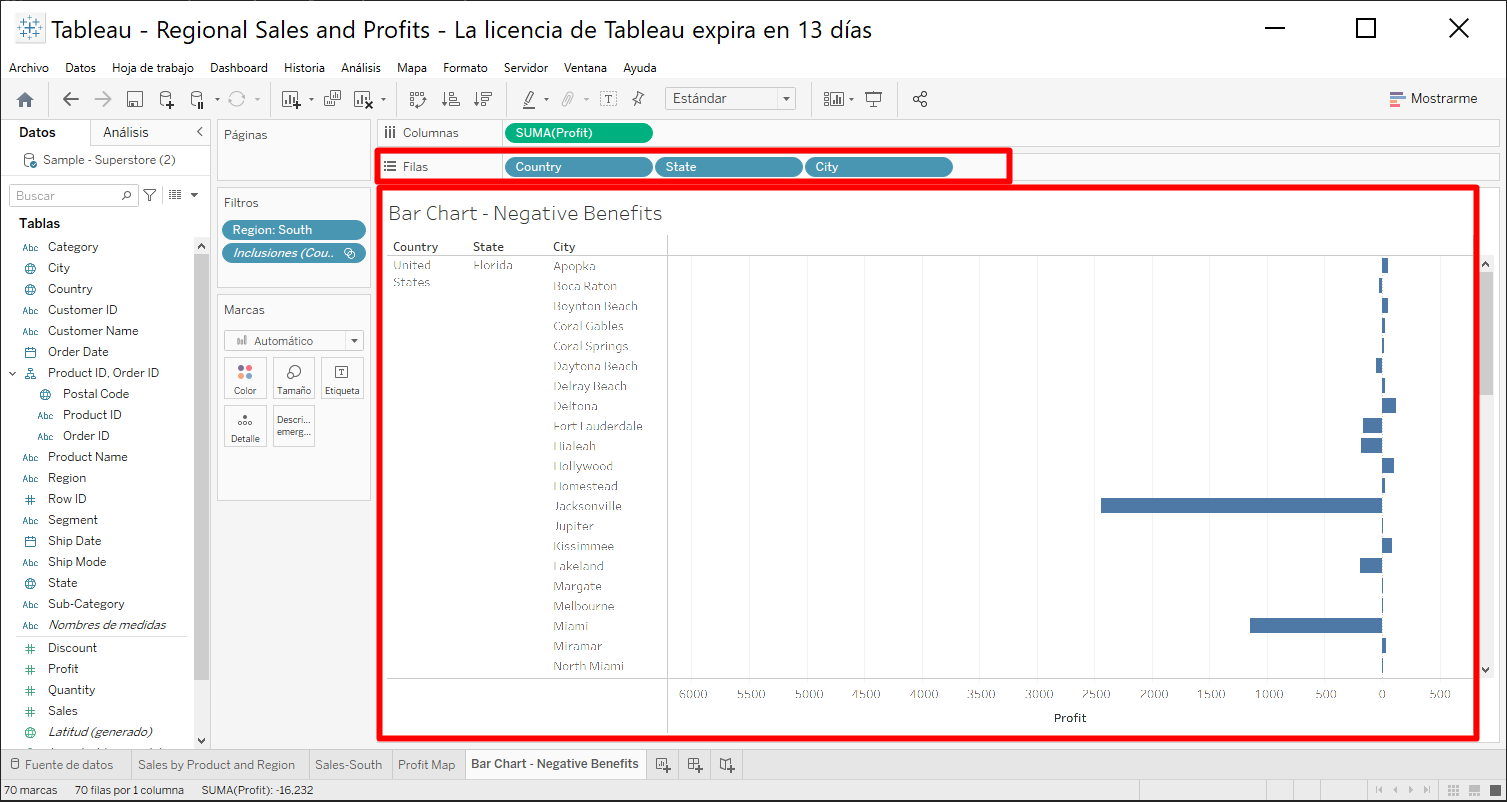
\includegraphics[width=16cm]{img/32.png}  
\end{center}
4. Eso es una gran cantidad de datos. Podemos usar N-Filter para filtrar y revelar los que tienen
un desempeño más débil. Para eso, arrastre Citydesde el Datapanel al estante Filtros. Haga
clic en el campo Por y luego haga clic en el Top menú desplegable y seleccione Bottom para
revelar los resultados más bajos . Escriba 5 en el cuadro de texto para mostrar los 5 mejores
resultados en el conjunto de datos.
\begin{center}
    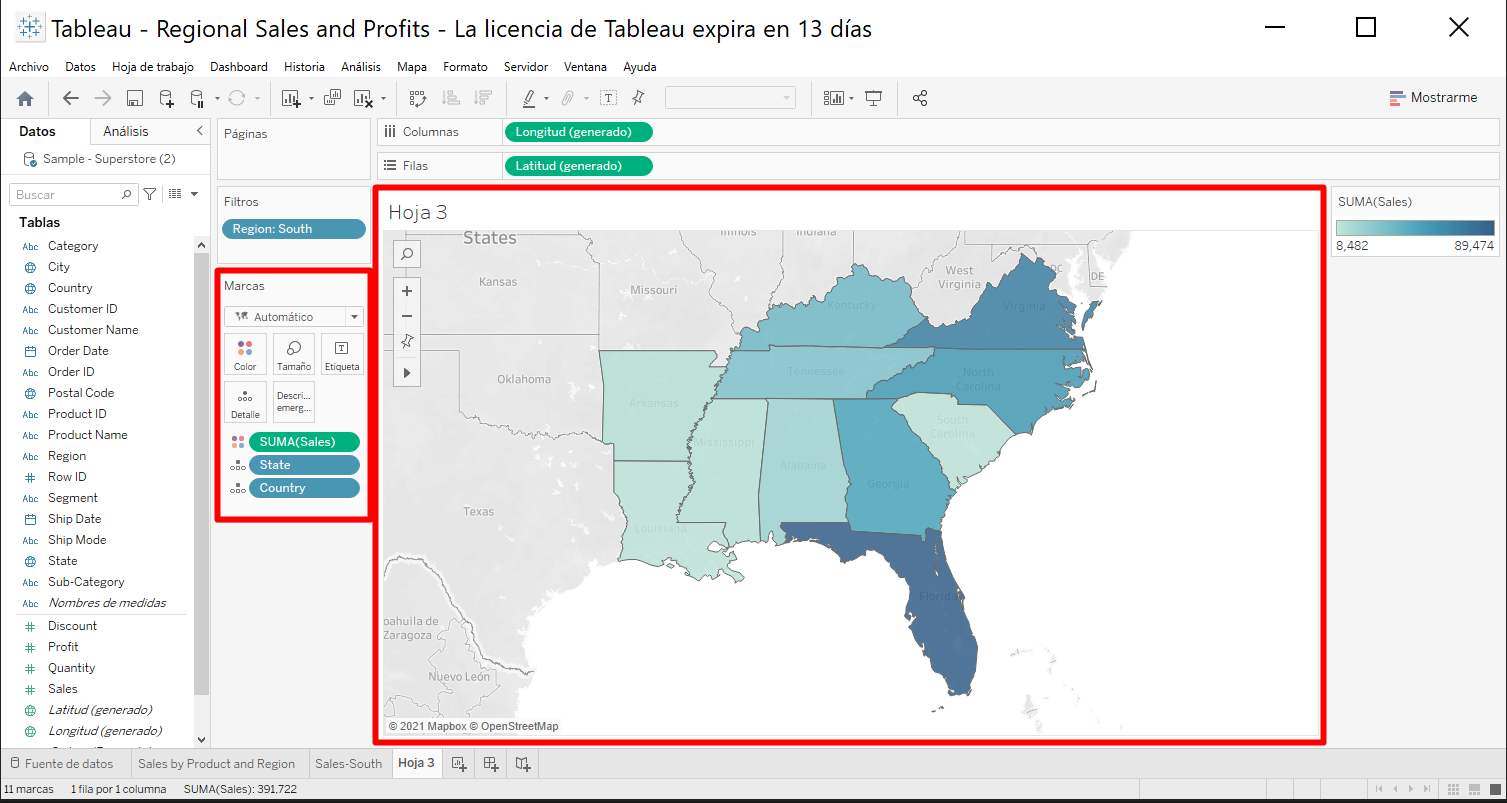
\includegraphics[width=10cm]{img/23.png}  
\end{center}
Ahora vemos que Jacksonville y Miami, Florida; Burlington, Carolina del Norte; y Knoxville y
Memphis, Tennessee, son las ciudades con peor desempeño en términos de ganancias. Hay otra
marca en la vista, Jacksonville, Carolina del Norte, que no pertenece aquí ya que tiene ventas 
rentables. Esto significa que hay un problema en el filtro que aplicamos. Aceptaremos la ayuda
de Tableau Order of Operations.
\begin{center}
    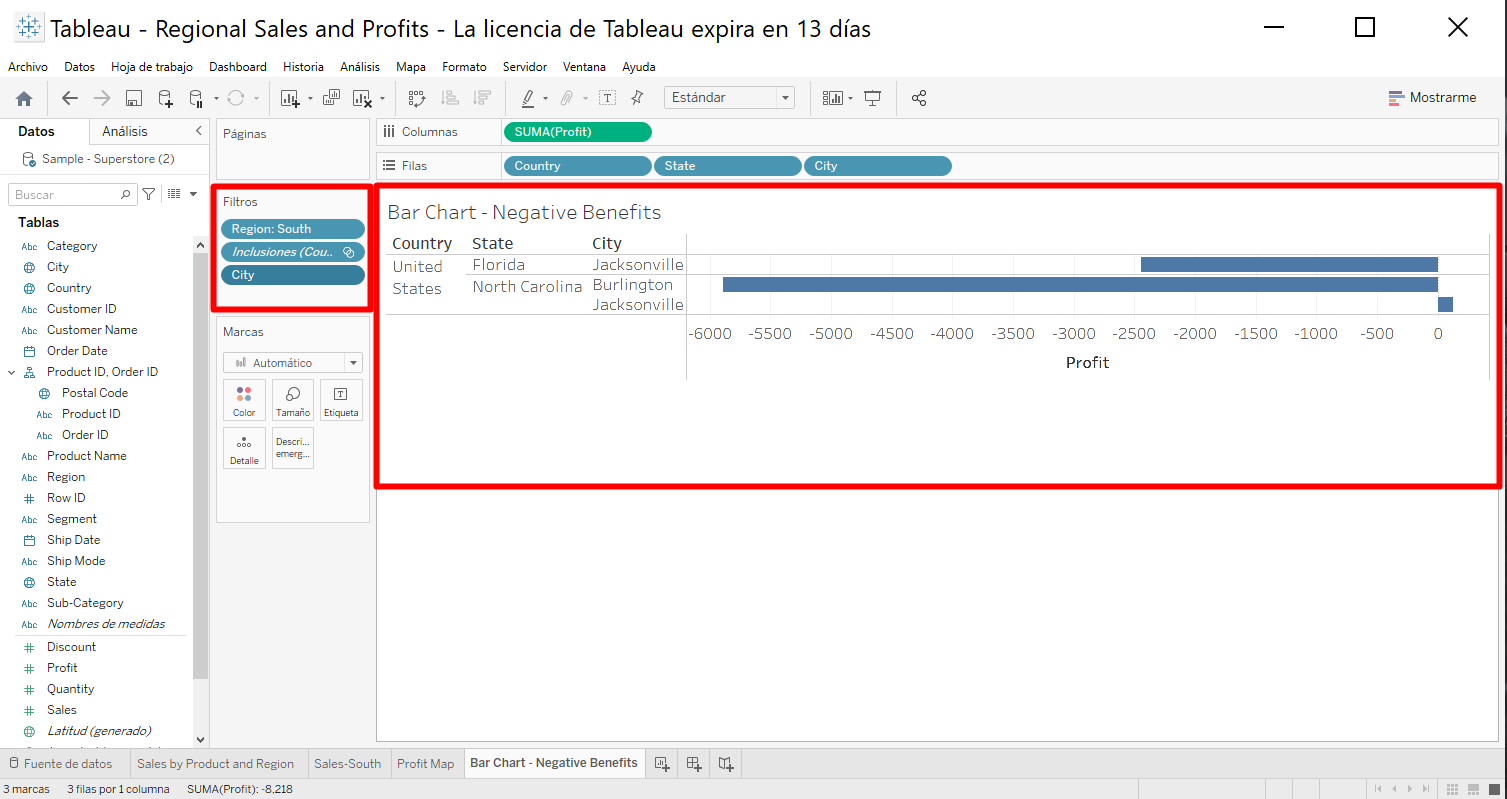
\includegraphics[width=16cm]{img/34.png}  
\end{center}
1. En el estante Filtros, haga clic con el botón derecho en el conjunto Inclusiones (país, estado) y
seleccione Add to Context. Encontramos que ahora Concord ( Carolina del Norte )
aparece a la vista mientras Miami ( Florida ) han desaparecido. Esto tiene sentido ahora.
\begin{center}
    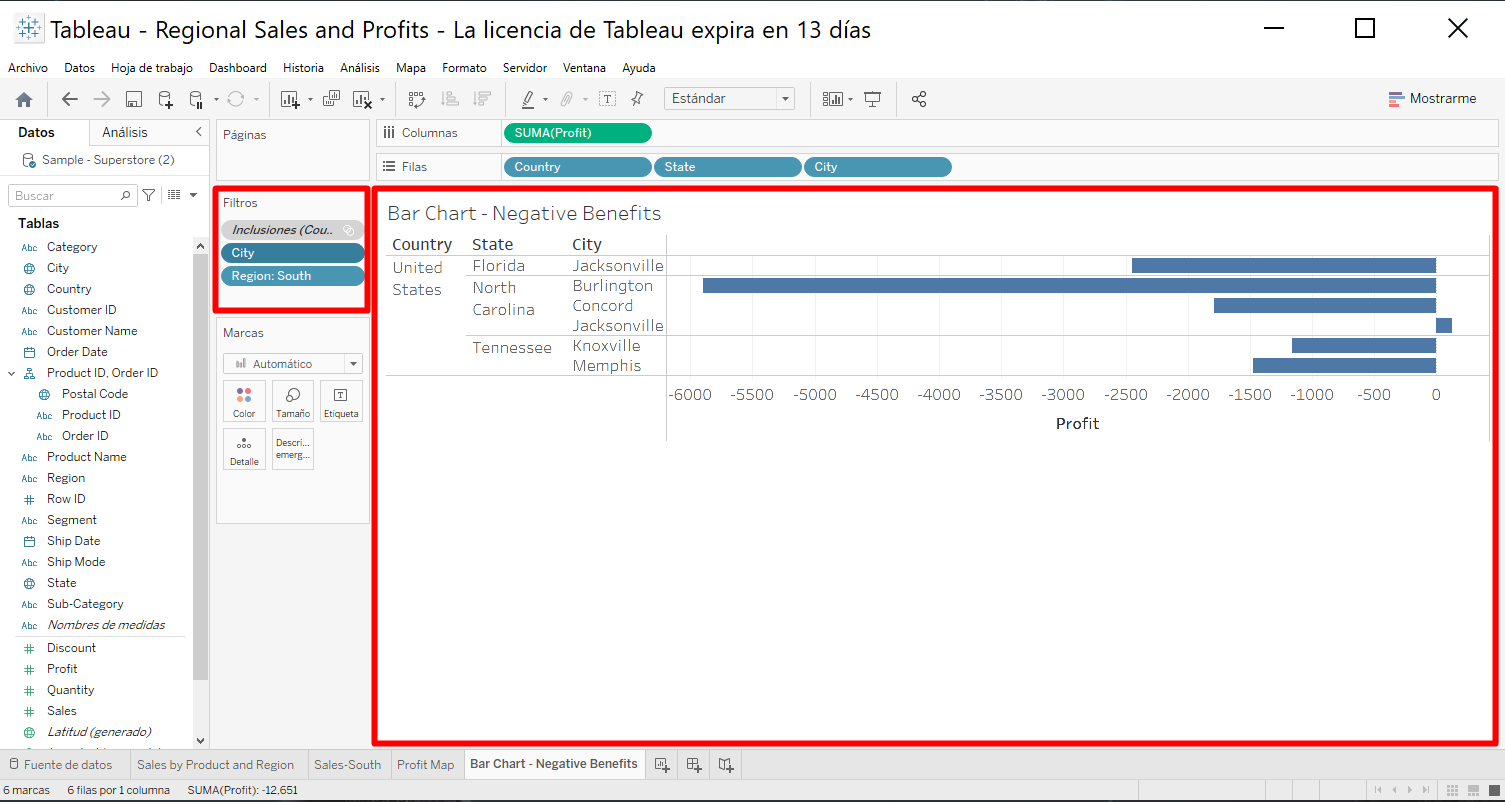
\includegraphics[width=16cm]{img/35.png}  
\end{center}
2. Pero Jacksonville ( Carolina del Norte ) todavía está presente, lo cual es incorrecto. En el
estante Filas, haga clic en el icono con forma de más en la Citypestaña para profundizar en el
nivel de Código postal. Haga clic con el botón derecho en el código postal de Jacksonville, NC,
28540, y luego seleccione Excludepara excluir Jacksonville manualmente.
\begin{center}
    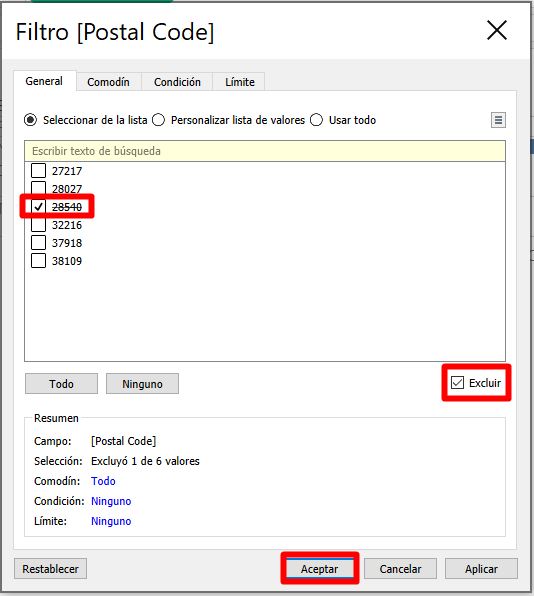
\includegraphics[width=10cm]{img/36.png}  
\end{center}
3. Arrastre Código postal del estante Filas. Esta es la vista final.
\begin{center}
    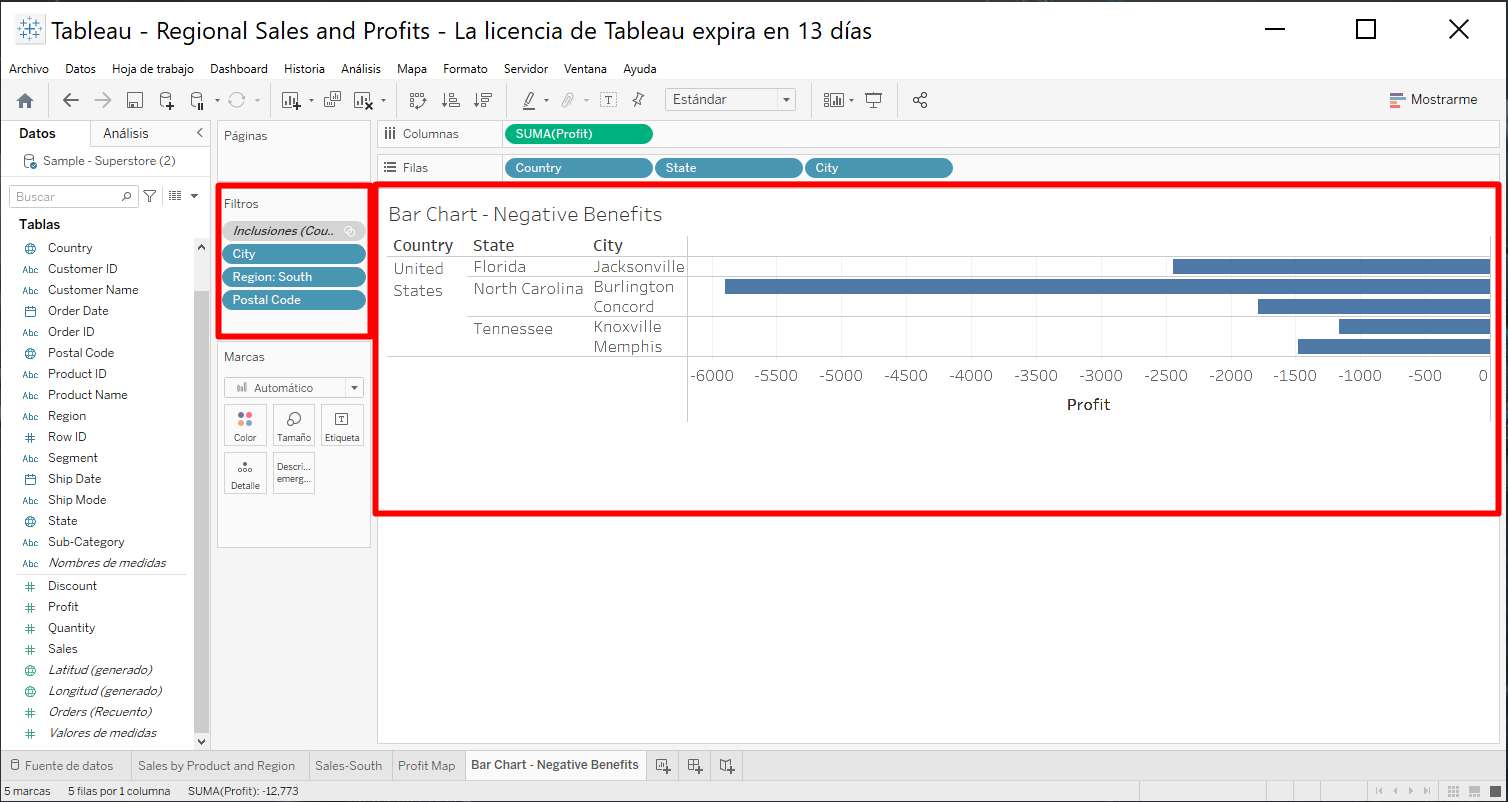
\includegraphics[width=16cm]{img/37.png}  
\end{center}

\subsection{Resultados clave}
Centrémonos ahora solo en las entidades que generan pérdidas, es decir, los
Productos y también identifiquemos las ubicaciones donde se venden dichos
productos.
\\\\STEPS:
\\\\1. Arrastre Sub-Categorya las Filas para profundizar más.
\begin{center}
    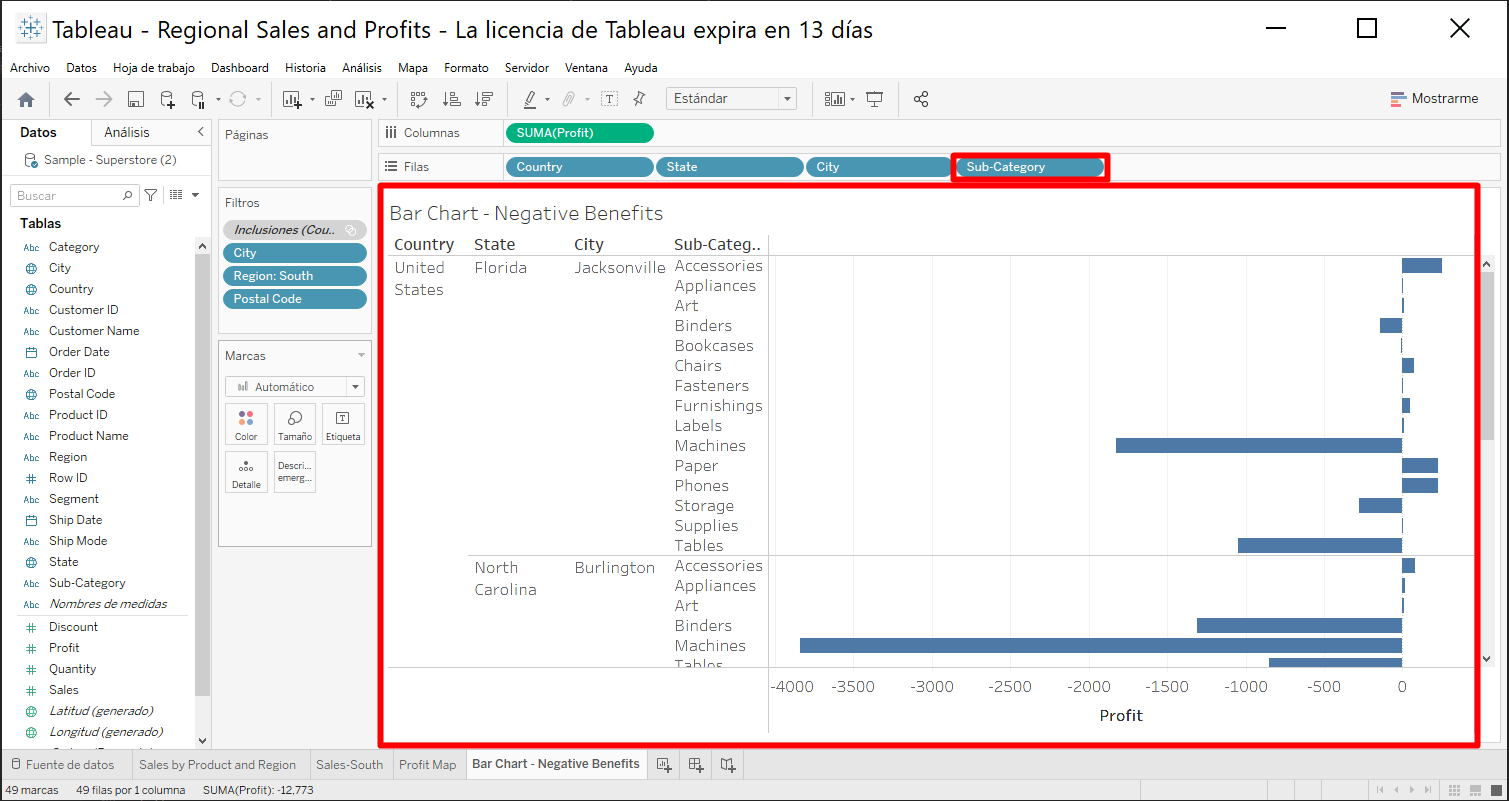
\includegraphics[width=16cm]{img/39.png}  
\end{center}
2. . Del mismo modo, arrastre Profithacia Coloren la tarjeta Marcas. Esto nos permite detectar
rápidamente productos con beneficios negativos.
\begin{center}
    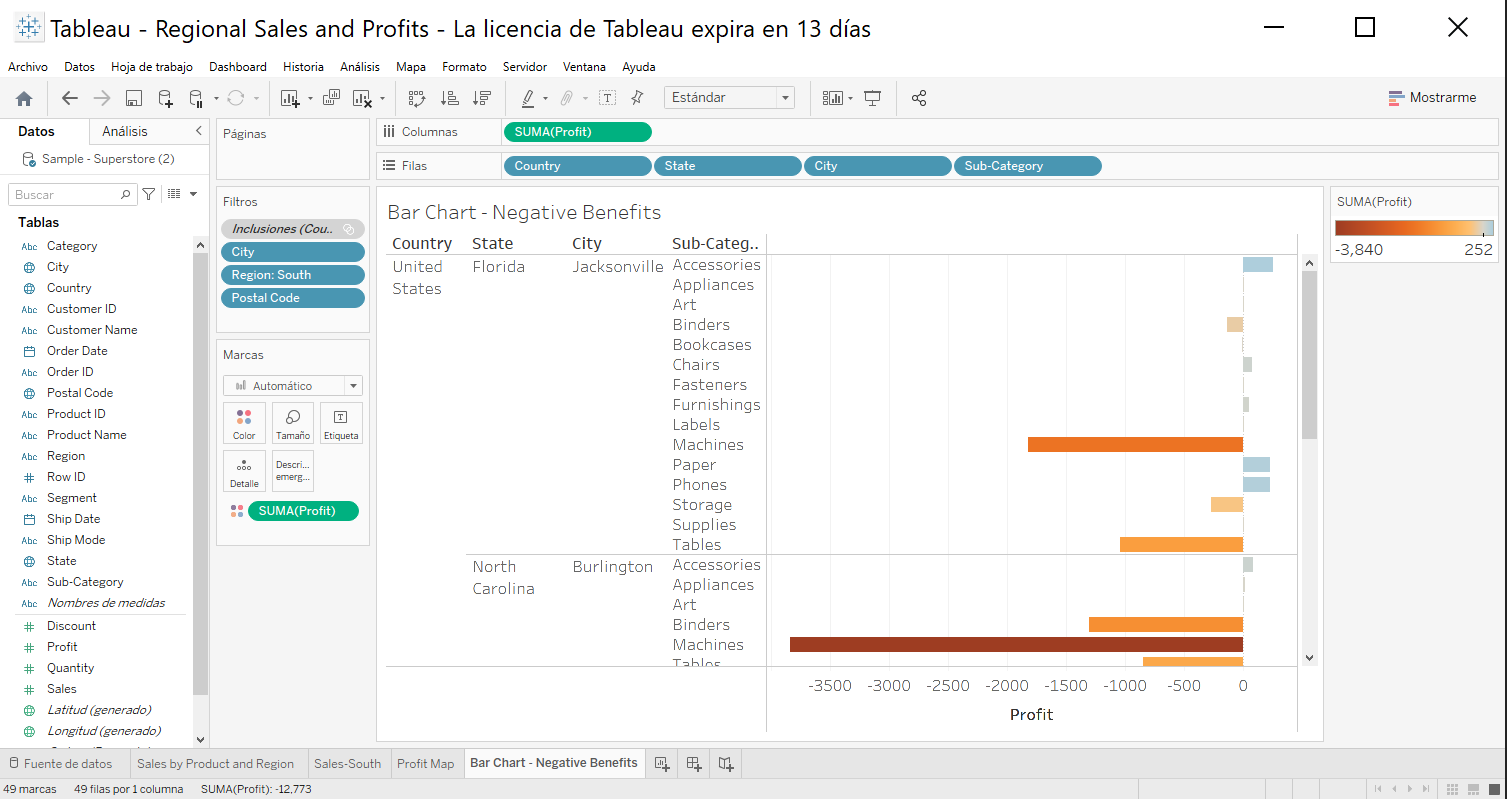
\includegraphics[width=16cm]{img/38.png}  
\end{center}
3. Haga clic derecho en Order Datey seleccione Show Filter. Parece que las máquinas, las
tablas y las carpetas funcionan mal. ¿Entonces, qué debemos hacer? ¿Una solución sería detener
la venta de estos productos en Jacksonville, Concord, Burlington, Knoxville y
Memphis? Verifiquemos si nuestra decisión es correcta.
\begin{center}
    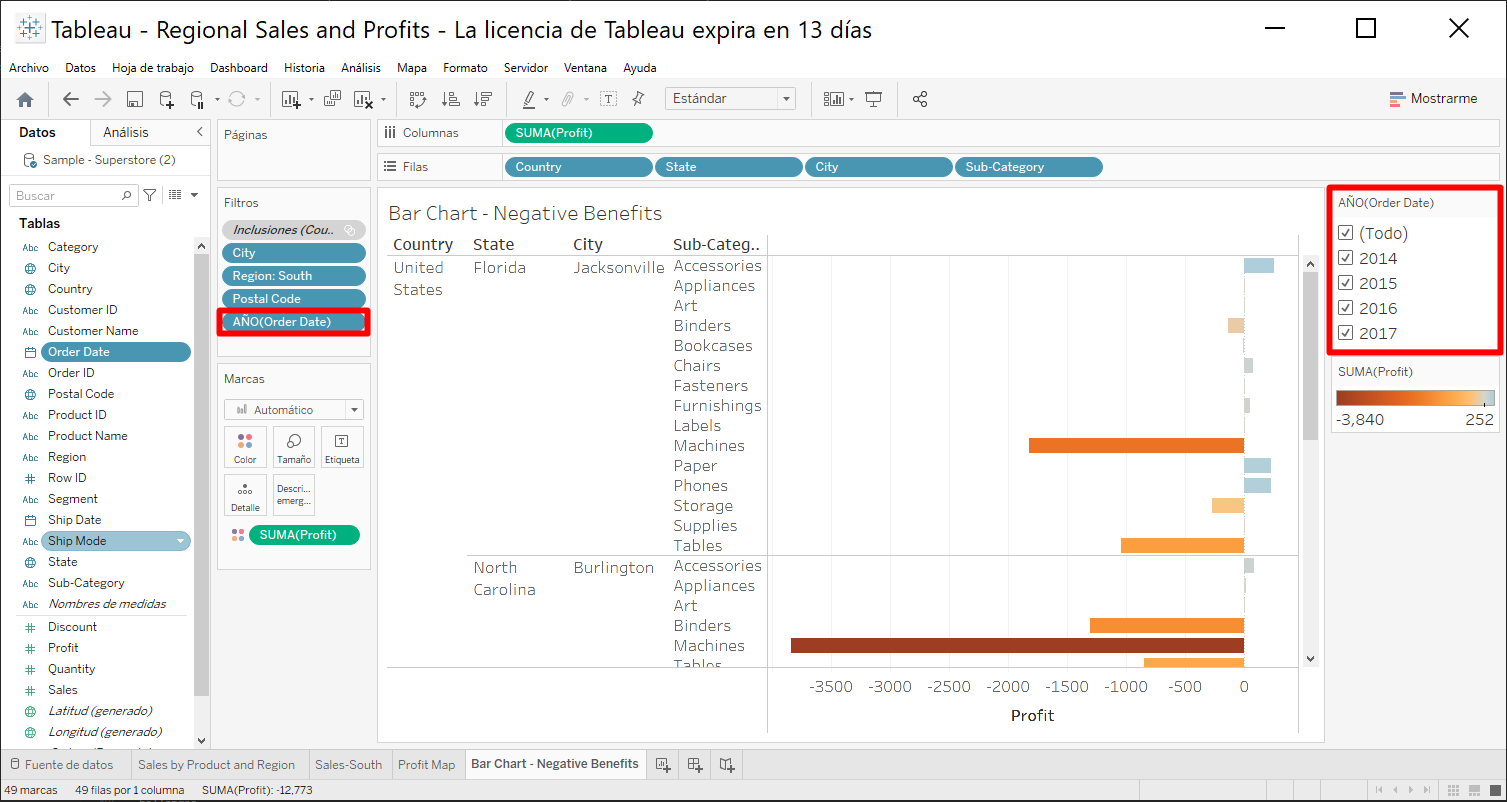
\includegraphics[width=16cm]{img/40.png}  
\end{center}
4. Regresemos a la Profit Map pestaña de la hoja creada anteriormente.
\begin{center}
    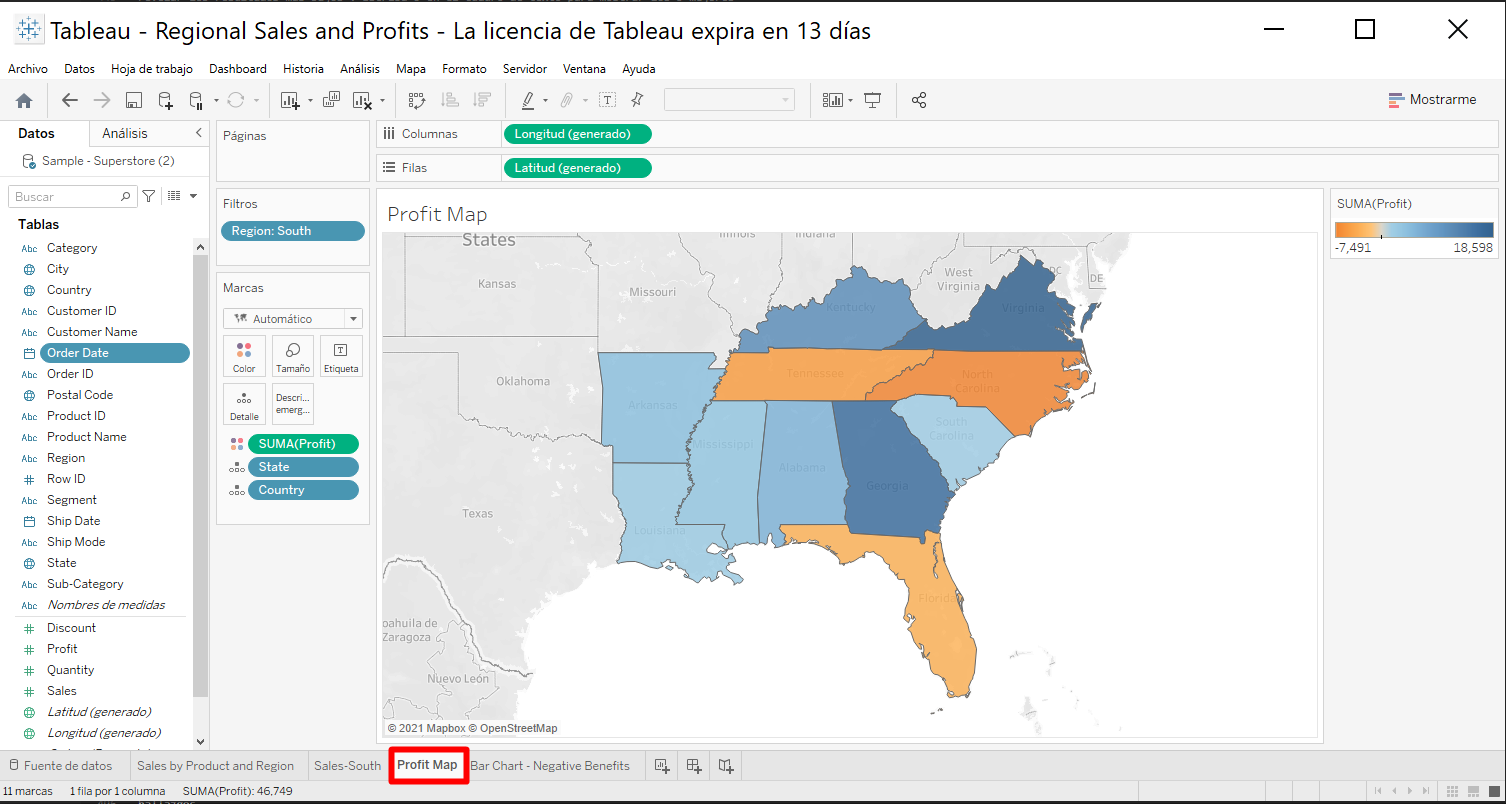
\includegraphics[width=16cm]{img/41.png}  
\end{center}
5. Ahora, haga clic en el Sub-Category campo para seleccionar la Show Filteropción.
\begin{center}
    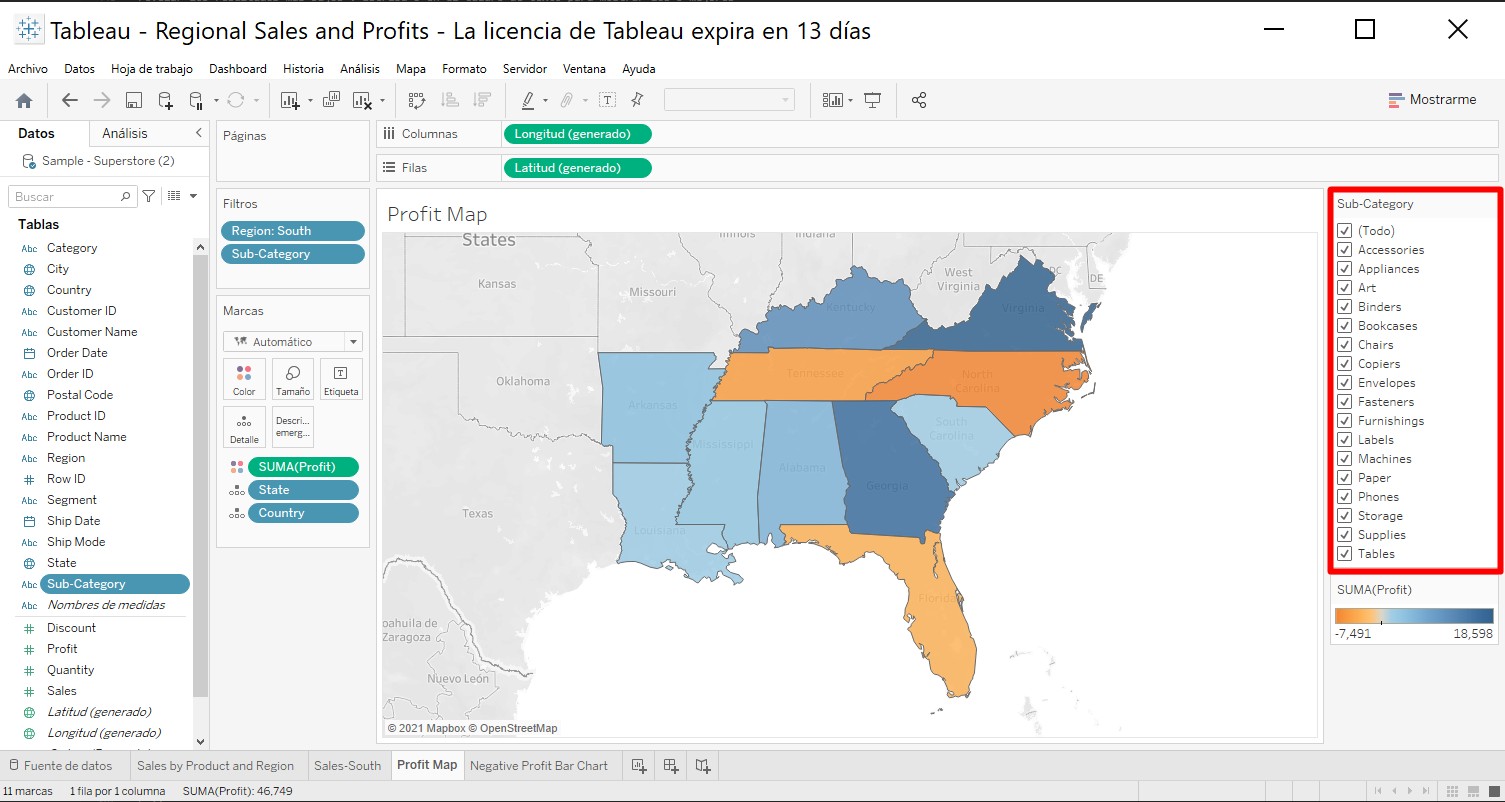
\includegraphics[width=16cm]{img/42.png}  
\end{center}
6. Arrastre Profit desde abajo Measures hasta la Labeltarjeta Marcas.
\begin{center}
    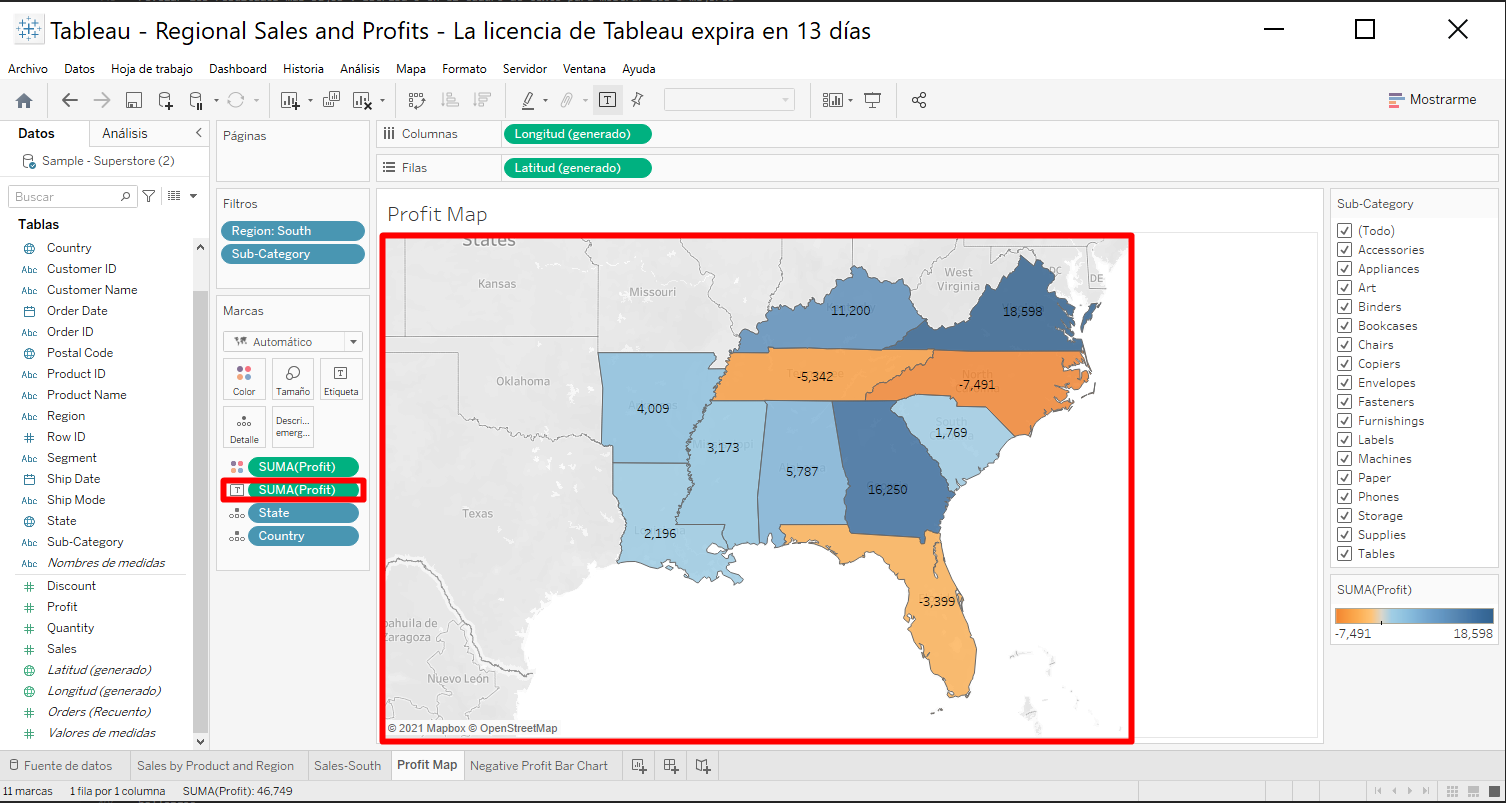
\includegraphics[width=16cm]{img/43.png}  
\end{center}
7. Nuevamente, haga clic en Order Datey seleccione Show Filter. Del filtro, eliminemos los
elementos que creemos que contribuyen al beneficio negativo. Por lo tanto, desmarque las 
casillas frente a Carpetas, Máquinas y Tablas, respectivamente. Ahora solo nos quedan las
entidades lucrativas. Esto muestra que las entidades como los aglutinantes, las máquinas y las
tablas en realidad estaban causando pérdidas en algunas áreas y teníamos razón en nuestros
hallazgos.
\begin{center}
    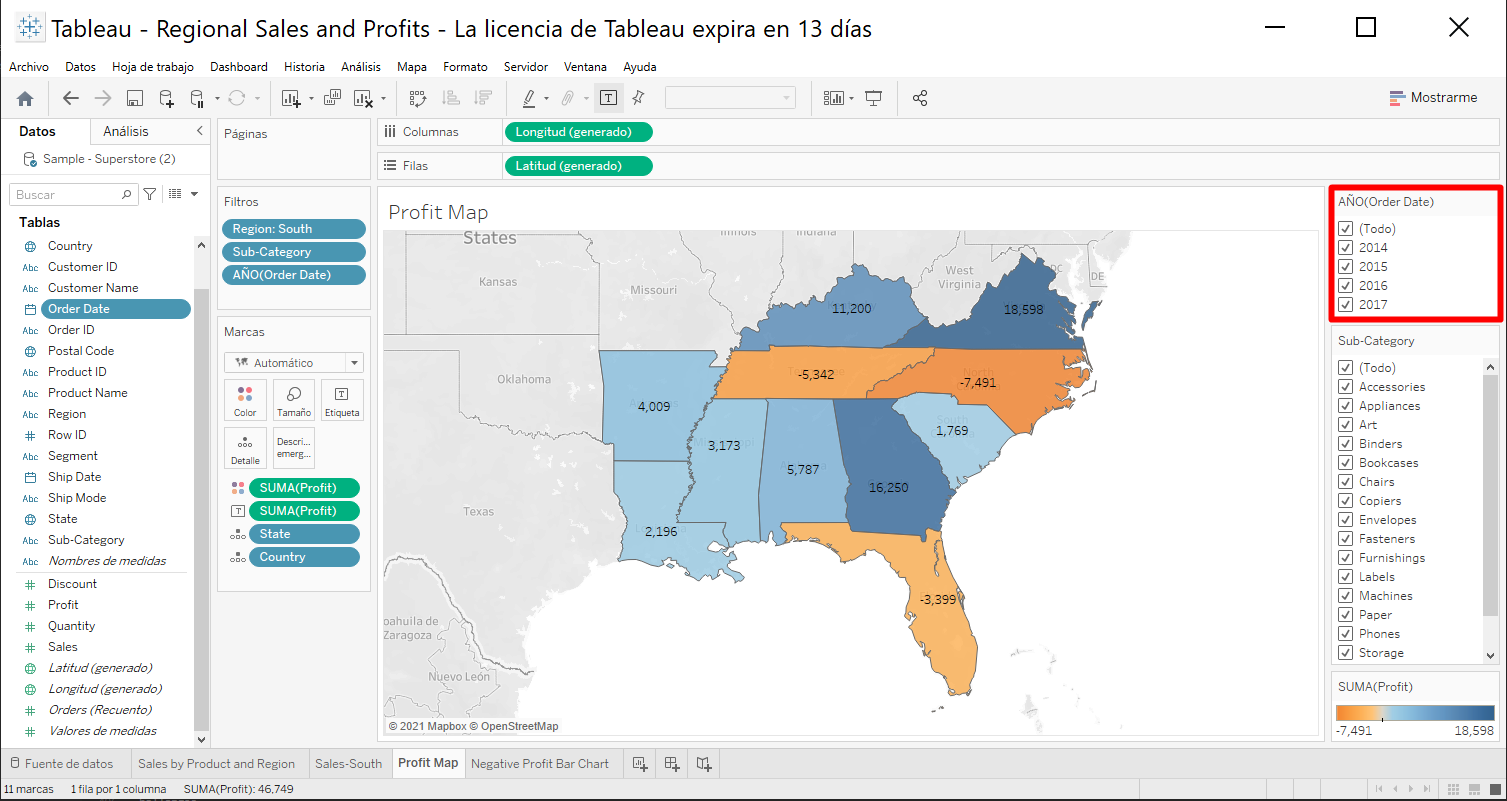
\includegraphics[width=16cm]{img/44.png}  
\end{center}
\begin{center}
    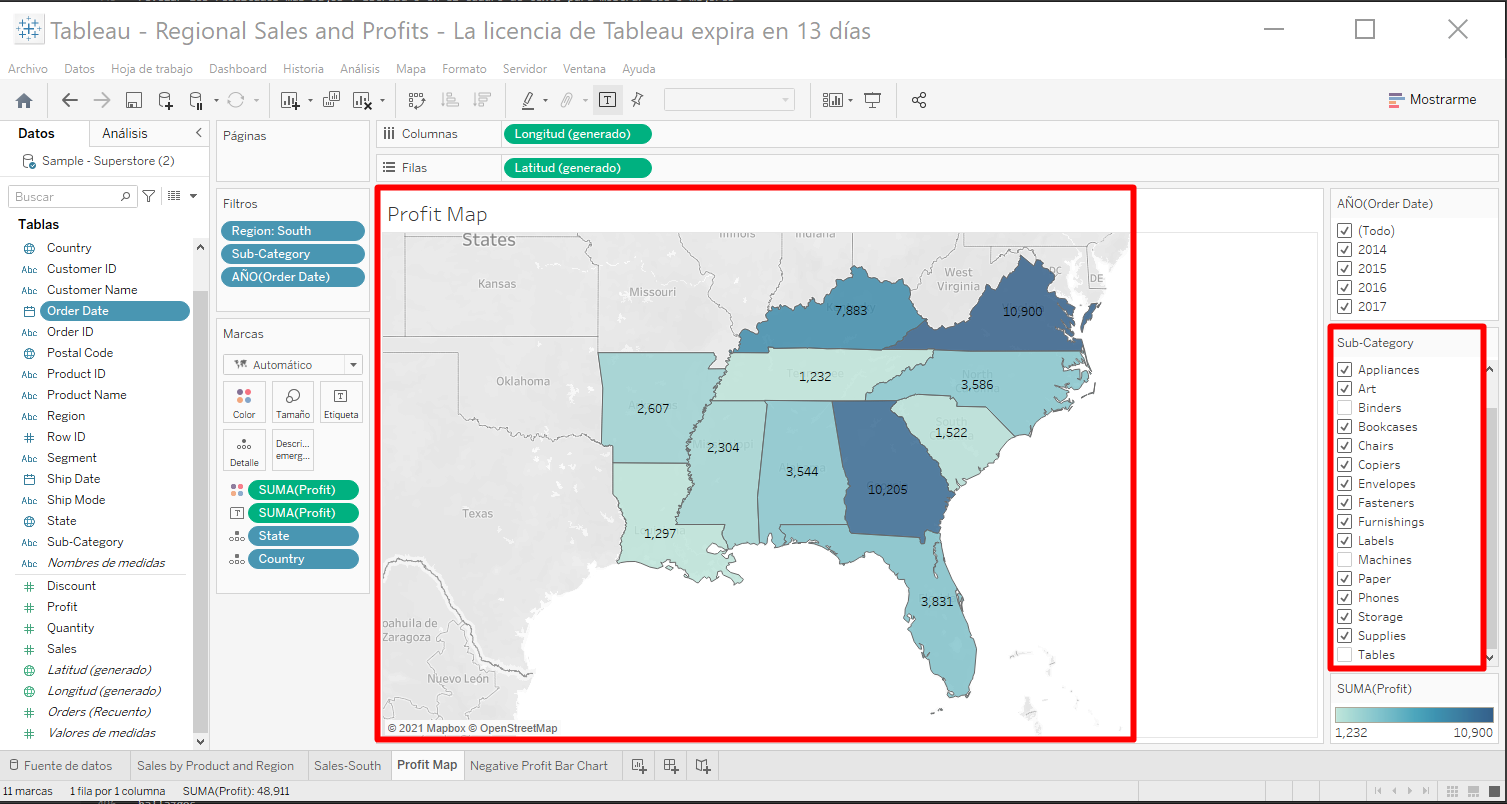
\includegraphics[width=16cm]{img/45.png}  
\end{center}

\section{Tablero}
Un tablero es una colección de varias vistas, lo que permite comparar una variedad de
datos simultáneamente.
\subsection{Crear un tablero}
STEPS:
\\\\1. Haga clic en el New dashboard botón.
\begin{center}
    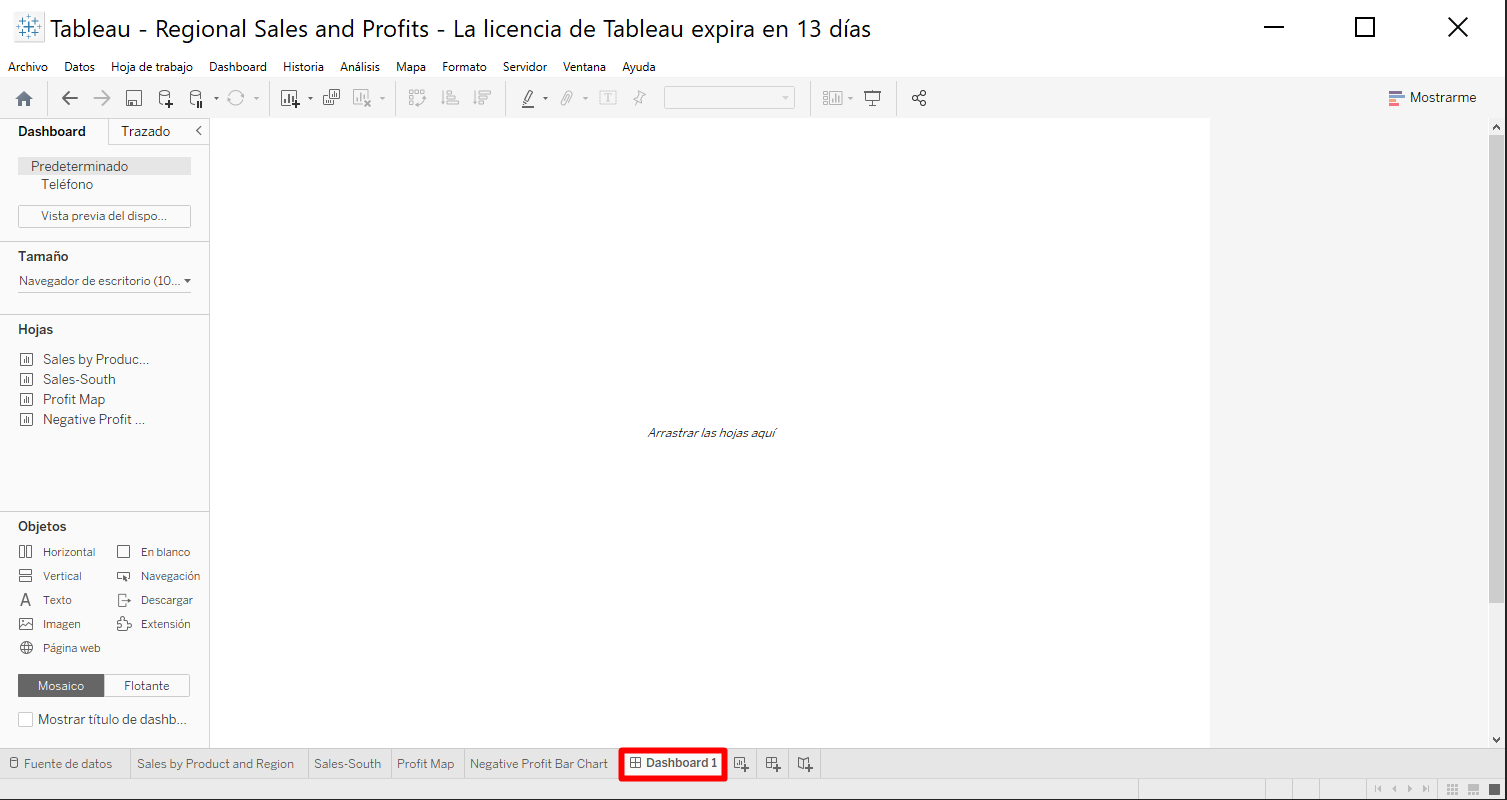
\includegraphics[width=16cm]{img/46.png}  
\end{center}
2. Arrastra Sales in the South al tablero vacío
\begin{center}
    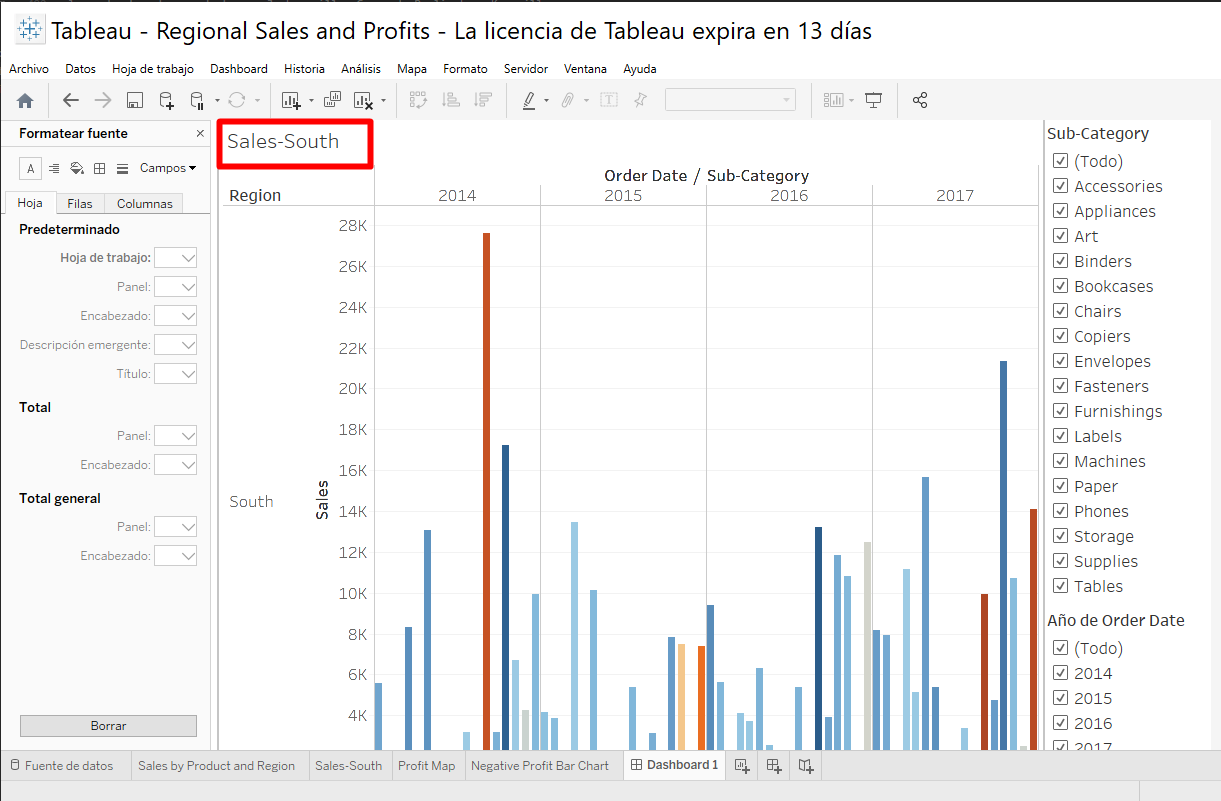
\includegraphics[width=16cm]{img/47.png}  
\end{center}
3. Arrastre Profit Map al tablero y suéltelo encima de Ventas en la vista Sur. Ambas vistas se
pueden ver a la vez. Para poder presentar los datos de manera que otros puedan entenderlos,
podemos organizar el tablero a nuestro gusto.
\begin{center}
    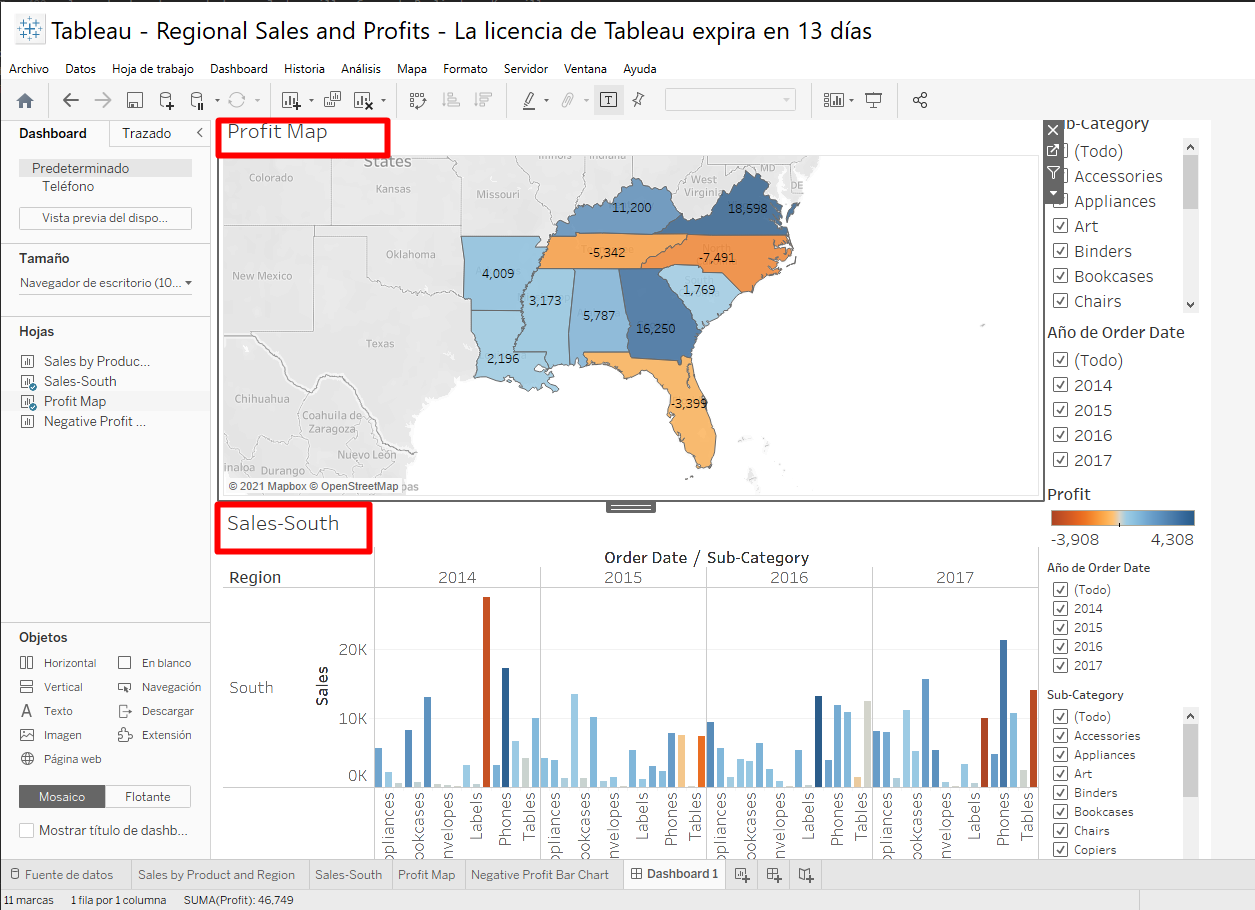
\includegraphics[width=16cm]{img/48.png}  
\end{center}
4. En la Sales Southhoja de trabajo en la vista del tablero, haga clic debajo de Region y
borre Show Header. Repita el mismo proceso para todos los demás encabezados. Esto ayuda a
enfatizar solo lo que se necesita y oculta la información no tan importante.
\begin{center}
    \includegraphics[width=16cm]{img/49.png}  
\end{center}
5. En el Profit Map, Ocultar el título también y realizar los mismos pasos para el Sales
South mapa.
\begin{center}
    \includegraphics[width=16cm]{img/50.png}  
\end{center}
6. Podemos ver que la Sub-Categorytarjeta de filtro y Year of Order Datese han repetido
en el lado derecho. Eliminemos los extras simplemente tachándolos. Finalmente, haga clic en
el Year of Order Date. Aparece una flecha desplegable y seleccione la opción de Single 
Value (Slider). Ahora deja que la magia se desarrolle. Experimente eligiendo diferentes
años en el control deslizante y las Ventas también variarán en consecuencia.
\begin{center}
    \includegraphics[width=16cm]{img/51.png}  
\end{center}
7. Arrastre el SUM(Profit) filtro a la parte inferior del panel debajo de Ventas en el sur para
obtener una mejor vista.
\begin{center}
    \includegraphics[width=16cm]{img/52.png}  
\end{center}

\subsection{Añadiendo interactividad}
Para que el panel de control sea más interactivo, como ver qué subcategorías son
rentables en qué estados, es necesario realizar algunos cambios.
\\\\STEPS:
\\\\1. Comencemos con el Profit Map. Al hacer clic en el mapa, Use as
filter aparece un icono en la parte superior derecha. Haz click en eso. Si seleccionamos
cualquier mapa, las Ventas correspondientes a ese estado se resaltarán en el Sales South mapa.
\begin{center}
    \includegraphics[width=16cm]{img/53.png}  
\end{center}
2. Para el Year of Order Date, haga clic en la opción desplegable y vaya a Apply to
Worksheets > Selected Worksheets. Se abre un cuadro de diálogo. Seleccione
la Allopción seguida de OK. ¿Qué hace esta opción? Aplica filtros a todas las hojas de trabajo
que tienen la misma fuente de datos.
\begin{center}
    \includegraphics[width=16cm]{img/54.png}  
\end{center}
\begin{center}
    \includegraphics[width=16cm]{img/55.png}  
\end{center}
3. Explore y experimente. En la visualización a continuación, podemos filtrar el Sales
South mapa para ver los productos que se venden solo en Carolina del Norte. Luego, podemos
explorar fácilmente las ganancias anuales.
\begin{center}
    \includegraphics[width=8cm]{img/56.png}  
\end{center}
\begin{center}
    \includegraphics[width=16cm]{img/57.png}  
\end{center}
4. Cambie el nombre del panel a Regional Sales and Profit.
\begin{center}
    \includegraphics[width=16cm]{img/58.png}  
\end{center}

\section{Historia}
Un tablero es una característica interesante, pero tableau también nos ofrece mostrar
nuestros resultados en el modo de presentación en forma de historias sobre las que
hablaremos en esta sección.
\subsection{Construyendo una historia}
STEPS:
\\\\1. Haga clic en el New story botón.
\begin{center}
    \includegraphics[width=16cm]{img/59.png}  
\end{center}
2. Desde el panel Historia a la izquierda, arrastre la Sales in the South hoja de trabajo
(creada anteriormente) a la vista.
\begin{center}
    \includegraphics[width=16cm]{img/60.png}  
\end{center}
3. Edite el texto en el cuadro gris sobre la hoja de trabajo. Este es el título. Nómbrelo como Sales
and profit by year.
\begin{center}
    \includegraphics[width=16cm]{img/61.png}  
\end{center}
4. Las historias son bastante específicas. Aquí contaremos una historia sobre la venta de máquinas
en Carolina del Norte. En el panel Historia, haga clic en Duplicate para duplicar el primer
título, o incluso puede crear uno nuevo.
\begin{center}
    \includegraphics[width=16cm]{img/62.png}  
\end{center}
5. En el Sub-Category, select solo filtro Machines. Esto ayuda a medir las ventas y los
beneficios de las máquinas por año.
\begin{center}
    \includegraphics[width=16cm]{img/63.png}  
\end{center}
6. Cambie el nombre del título a Machine sales and profit by year.
\begin{center}
    \includegraphics[width=16cm]{img/64.png}  
\end{center}

\subsection{Hacer una conclusion}
Está claro que las máquinas en Carolina del Norte están provocando pérdidas de
beneficios. Sin embargo, esto no se puede demostrar observando las ganancias y las
ventas en su conjunto. Para ello, necesitamos Beneficio regional.
\\\\STEPS:
1. En el panel Historia, seleccione Blank. Arrastre el panel ya creado Regional Sales and
Profit al lienzo.
\begin{center}
    \includegraphics[width=16cm]{img/65.png}  
\end{center}
2. Subtitúlelo como Low performing items in the South.
\begin{center}
    \includegraphics[width=16cm]{img/66.png}  
\end{center}
3. Seleccione Duplicate para crear otro punto de la historia con el panel de ganancias
regionales. Seleccione Carolina del Norte en el gráfico de barras, ya que estamos interesados en
mostrar más al respecto.
\begin{center}
    \includegraphics[width=16cm]{img/67.png}  
\end{center}
4. Seleccione Todos los años.
\begin{center}
    \includegraphics[width=16cm]{img/68.png}  
\end{center}
5. Agregar un título para mayor claridad, como, Profit in NC : 2013-2016.
\begin{center}
    \includegraphics[width=16cm]{img/69.png}  
\end{center}
6. Seleccione cualquier año como 2014. Agregue un título, por ejemplo, Profit in NC :
2014 y luego haga clic en la pestaña Duplicar. Repita el mismo paso para todos los años
restantes.
\begin{center}
    \includegraphics[width=16cm]{img/70.png}  
\end{center}
7. Haz clic en el modo de presentación y deja que se story desarrolle.
\begin{center}
    \includegraphics[width=16cm]{img/71.png}  
\end{center}
Ahora tenemos una idea acerca de qué productos se introdujeron en el mercado de
Carolina del Norte, cuándo y cómo funcionaron. No solo hemos identificado una forma
de abordar las ganancias negativas, sino que también hemos logrado respaldarlas con
datos. Ésta es la ventaja de Story en Tableau.

\section{Integración de Tableau con R, Python y SQL}
Además de las diversas ventajas de visualización que ofrece Tableau, también tiene una increíble
capacidad de conexión lista para usar. Tableau puede integrarse fácilmente con lenguajes como Python
y R e incluso con DBMS como SQL. Esto ofrece mayores ventajas en cuanto a funcionalidades y
resulta útil para los científicos de datos que están acostumbrados a trabajar en Python o R. Pueden
importar directamente los scripts de R y Python en Tableau y aprovechar sus visualizaciones, que son
mucho más superiores a las de estos lenguajes. . Además, las capacidades de visualización de tableau
son fáciles de usar y muy intuitivas, lo que ahorra mucho tiempo a los científicos de datos.
\\\\En esta sección, veremos cómo podemos conectar Tableau con estas fuentes externas y las ventajas de
estas conexiones.
\subsection{Tableau y R}
R es un lenguaje estadístico popular que se utiliza para realizar análisis predictivos sofisticados, como
modelos lineales y no lineales, pruebas estadísticas, análisis de series de tiempo, clasificación,
agrupamiento, etc. (Tableau 8.1 y R). El uso de Tableau junto con R tiene las siguientes ventajas:
\\\\• Aprovecha el poder estadístico de Tableau al brindar a sus usuarios acceso a sofisticadas
bibliotecas de R para obtener información mejor y más profunda de los datos.
\\\\• Las opciones mejoradas de exploración de datos de Tableaus y la capacidad de conectarse a
múltiples fuentes resultan útiles para los usuarios de R.
\\\\• Además, también permite a los usuarios de Tableau beneficiarse de la utilidad del lenguaje R
sin tener que conocer realmente el lenguaje.
\\\\¿COMO SE INTEGRA TABLEAU CON R?
\\\\Las funciones y modelos R se pueden usar en Tableau creando nuevos campos calculados que invocan
dinámicamente el motor R y pasan valores a R. Estos resultados luego se devuelven a Tableau para
usarse con fines de visualización.
\\\\CONFIGURACION DE TABLEAU DESKTOP CON R
\\\\Descargar e instalar Rserve.
\\\\Deberá descargar e instalar el Rserve paquete para que Tableau se conecte y utilice las funciones del
script R. En la consola R, ingrese los siguientes comandos:
\\install.packages("Rserve")
\\setwd("C:/Program Files/R/R-4.0.4/bin/x64")
\\library(Rserve)
\\Rserve()
\begin{center}
    \includegraphics[width=16cm]{img/72.png}  
\end{center}

CONECTE TABLEAU AL SERVIDOR R
\\\\Una vez que Rserve se haya instalado correctamente, abra Tableau Desktop y siga los pasos que se
mencionan a continuación.
\\\\1. Vaya al Help > Settings and Preferences and select Manage External
Service Connection.
\begin{center}
    \includegraphics[width=8cm]{img/73.png}  
\end{center}
2. Introduzca el nombre del servidor como “Localhost” (o “127.0.0.1”) y un puerto de “6311”.
\begin{center}
    \includegraphics[width=8cm]{img/74.png}  
\end{center}
3. Haga clic en el botón "Probar conexión". Debería ver un mensaje de solicitud correcto. Haga
clic en Aceptar para cerrar.
\begin{center}
    \includegraphics[width=8cm]{img/75.png}  
\end{center}

COMIENCE A USAR LOS SCRIPTS DE R EN TABLEAU
\\\\Después de completar con éxito los pasos anteriores, podremos crear nuevos campos calculados en
Tableau Desktop que utilizan las funciones SCRIPT\_ * para realizar llamadas funcionales R.
\\\\Pongámonos manos a la obra y veamos cómo podemos usar las capacidades de Tableau con R.
Utilizaremos el conjunto de datos de Sample Superstore incorporado para calcular el beneficio tanto
mediante el script R como con la función de arrastrar y soltar de Tableau. Luego compararemos ambos
resultados.


\end{document}

